\NeedsTeXFormat{LaTeX2e}[2005/12/01]
%%    2009/03/12 v1.0 GAUBM Vorlage für Aschlussarbeiten Physik
%% Template fuer Bachelor- und Masterarbeiten
%% an der Fakultaet fuer Physik (c) Thomas Pruschke der GA Universität
%% Verbesserungsvorschlaege bitte an pruschke@theorie.physik.uni-goettingen.de
%%
%% Benoetigte Pakete: datenumber
%%

%%%%%%%%%%%%%%%%%%%%%%%%%%%%%%%%%%%%%%%%%%%%%%%%%%%%%%%%%%%%%%%%%%%%%%
%%%%%%%%%% Bitte vor dem Veraendern diese Datei umbenennen! %%%%%%%%%%
%%%%%%%%%%%%%%%%%%%%%%%%%%%%%%%%%%%%%%%%%%%%%%%%%%%%%%%%%%%%%%%%%%%%%%

%% scrbook - Ersatz für LaTeX book Klasse aus dem KOMA Script
%% Moegliche Optionen: diejenigen der Klasse scrbook ausser titlepage

%% deutsche Arbeit:
\documentclass[bachelor,       %% Typ der Arbeit: bachelor oder master
               twoside,        %% zweiseitiges Layout
               BCOR10mm,       %% Bindekorrektur 10 mm
               liststotoc,nomtotoc,bibtotoc, %% Aufnahme der div. Verzeichnisse
                                              %% ins Inhaltsverzeichnis
               english,ngerman, %% Alternativspr. Englisch, Dokumentspr. Deutsch
%               ngerman,english  %% Alternativspr. Deutsch, Dokumentspr. Englisch
               final,          %% Endversion; draft fuer schnelles Kompilieren
               ]{GAUBM}

\usepackage{setspace}  %% Zur Setzung des Zeilenabstandes
\usepackage[english,ngerman]{babel}     %% Sprachen-Unterstuetzung
\usepackage{calc}      %% ermoeglicht Rechnen mit Laengen und Zaehlern
\usepackage[T1]{fontenc}       %% Unterstutzung von Umlauten etc.
%\usepackage[latin1]{inputenc}  %% 
%% in aktuellem Linux & MacOS X wird standardmaessig UTF8 kodiert!
\usepackage[utf8]{inputenc}    %% Wenn latin1 nicht geht ...

\usepackage{emptypage} %% leere Seiten sind dann wirklich leer

\usepackage{amsmath,amssymb} %% zusaetzliche Mathe-Symbole

\usepackage{lmodern} %% type1-taugliche CM-Schrift als Variante zur
                     %% "normalen" EC-Schrift
%% Paket fuer bibtex-Datenbanken
%\usepackage[comma,numbers,sort&compress]{natbib}
\usepackage{babelbib}
\selectbiblanguage{ngerman}
\bibliographystyle{apalikeGerman}

\newcommand{\tabheadfont}[1]{\textbf{#1}} %% Tabellenkopf in Fett
\usepackage{booktabs}                      %% Befehle fuer besseres Tabellenlayout
\usepackage{longtable}                     %% umbrechbare Tabellen
\usepackage{array}                         %% zusaetzliche Spaltenoptionen

%% umfangreiche Pakete fuer Symbole wie \micro, \ohm, \degree, \celsius etc.
\usepackage{textcomp,gensymb}
\usepackage{wasysym}

%\usepackage{SIunits} %% Korrektes Setzen von Einheiten
\usepackage{units}   %% Variante fuer Einheiten
\usepackage{xcolor}
%% Hyperlinks im Dokument; muss als eines der letzten Pakete geladen werden
\usepackage[pdfstartview=FitH,      % Oeffnen mit fit width
            breaklinks=true,        % Umbrueche in Links, nur bei pdflatex default
            bookmarksopen=true,     % aufgeklappte Bookmarks
            bookmarksnumbered=true  % Kapitelnummerierung in bookmarks
            ]{hyperref}

%% Weiter benoetigte Pakete: datenumber
%% Falls dieses Paket nicht in der Installation vorhanden ist,
%% kann es von der Seite mit diesem Template heruntergeladen werden
%% und in einem LaTeX bekanntem Verzeichnis installiert werden (notfalls
%% dem Verzeichnis mit der Arbeit).

% Mehrere Abbildungen nebeneinander
\usepackage{subfig}
\usepackage{adjustbox}

%Boxen,etc.
\usepackage{fancybox}
\usepackage{empheq}

% SI-Paket
\usepackage{siunitx}

%Matlab-Code
%\usepackage{listings}
\usepackage[framed,numbered]{matlab-prettifier}

\newcommand{\dif}{\ensuremath{\mathrm{d}}}

\begin{document}
%%
%%                   Ab hier muessen die Anpassungen geschehen
%%
%% Hier den eigenen Namen einsetzen
\ThesisAuthor{Felix}{Kurtz}
%% Hier den Geburtsort einsetzen
\PlaceOfBirth{Bad Nauheim}
%% Titel Arbeit. Das erste Argument ist der deutsche, das zweite der
%% englische Titel.
\ThesisTitle{Echtzeit-Spektroskopie der Multipuls-Dynamik in einem Ti:Sa-Femtosekunden-Oszillator}{Real-time spectroscopy of\\ multipulse dynamics in a \\Ti:Sapph femtosecond oscillator}
%% Erst- und Zweitgutacher/in
%% Ist der/die Betreuer/in nicht identisch mit dem/r Erstgutachter/in,
%% muss diese/r als optionales Argument angegeben werden.
\FirstReferee[Dr.\ Georg Herink]{Prof.\ Dr.\ Claus Ropers}
\Institute{4.\,Physikalischen Institut}
\SecondReferee{Prof.\ Dr.\ Stefan Mathias}
%% Beginn und Ende des Anfertigungszeitraumes
\ThesisBegin{1}{4}{2016}
\ThesisEnd{15}{7}{2016}
%% DO NOT TOUCH THESE LINES!!!!
\frontmatter
\maketitle
\cleardoublepage
%% Zusammenfassung. Falls nicht gewuenscht, bitte auskommentieren.
\begin{abstract}
In dieser Arbeit wird das Spektrum eines 80\,MHz-Ti:Sa-Oszillators in Echtzeit gemessen.
Dazu wird mit Hilfe einer dispersiven Faser spektrale Information in zeitliche Information übersetzt, die dann mit Hochgeschwindigkeitselektronik aufgezeichnet wird.
Dies wird genutzt, um Multipuls-Dynamiken zu enthüllen, die sich bei bestimmten Justagen des Laserresonators einstellen.
Vor allem Doppelpulse stehen hierbei im Fokus.
Aus dem zugehörigen Spektrum lässt sich der Abstand sowie die relative Phase beider Pulse bestimmen.
So werden unterschiedlichste Dynamiken beobachtet: 
Abstand und relative Phase oszillieren, die relative Phase wächst stufenweise an, die Pulse kollidieren unentwegt, aber auch unterschiedlich schnelle Pulse, die annähernd unabhängig durch den Resonator laufen.
Darüber hinaus werden diskrete Werte für stabile Pulsabstände identifiziert.
Mit Simulationen werden einige Dynamiken nachvollzogen.
%% Optional: Stichwoerter. Wenn nicht gewuenscht, koennen die beiden
%% folgenden Zeilen geloescht werden
  \bigskip\par
  \textbf{Stichwörter:} Physik, Bachelorarbeit
\end{abstract}
%% So laesst sich in die andere Sprache umschalten (Englisch bzw. Deutsch)
\begin{otherlanguage}{english}
\begin{abstract}
  Here the key results of the thesis can be presented in about
  half a page.
  \bigskip\par
  \textbf{Keywords:} Physics, Bachelor thesis
\end{abstract}
\end{otherlanguage}

%% Ende des Vorspanns
\cleardoublepage
%% Ab hier 1 1/2 facher Zeilenabstand (durch setspace-Paket)
\onehalfspacing
%% Erzeugt Inhaltsverzeichnis
\tableofcontents

%%% Hier kann man seine Bezeichnungsweisen erklaeren. Falls nicht
%%% benoetigt, bis einschliesslich \end{nomenclature} auskommentieren
%\begin{nomenclature}
%%% Fuer die Berechnung der Spaltenbreiten muss \usepackage{calc}
%%% geladen sein!
%\section*{Lateinische Buchstaben}
%\noindent
%\begin{longtable}[l]{p{0.2\textwidth}p{0.7\textwidth-6\tabcolsep}p{0.1\textwidth}}
%  \tabheadfont{Variable}&\tabheadfont{Bedeutung}&\tabheadfont{Einheit}\\\midrule\endhead
%  $A$ & Querschnittsfl"ache & $\unit{m^2}$\\
%  $c$ & Geschwindigkeit & $\unitfrac{m}{s}$
%\end{longtable}
%\section*{Griechische Buchstaben}
%\begin{longtable}[l]{p{0.2\textwidth}p{0.7\textwidth-6\tabcolsep}p{0.1\textwidth}}
%  \tabheadfont{Variable}&\tabheadfont{Bedeutung}&\tabheadfont{Einheit}\\\midrule\endhead
%  $\alpha$  & Winkel & $\unit{\degree}$; --\\
%  $\varrho$ & Dichte & $\unitfrac{kg}{m^3}$
%\end{longtable}
%\section*{Indizes}
%\begin{longtable}[l]{p{0.2\textwidth}p{0.8\textwidth-4\tabcolsep}}
%  \tabheadfont{Index}&\tabheadfont{Bedeutung}\\\midrule\endhead
%  m & Meridian\\
%  $r$ & Radial
%\end{longtable}
%\section*{Abk"urzungen}
%\begin{longtable}[l]{p{0.2\textwidth}p{0.8\textwidth-4\tabcolsep}}
%  \tabheadfont{Abk"urzung}&\tabheadfont{Bedeutung}\\\midrule\endhead
%  2D & zweidimensional\\
%  3D & dreidimensional\\
%  max & maximal
%\end{longtable}
%\end{nomenclature}
%% \listoftables und \listoffigures sollten nur bei genuegender Anzahl Tabellen
%% verwendet werden
%\listoffigures
%\listoftables

\mainmatter   %% Anfang Hauptteil

\chapter{Einleitung}
Femtosekundenlaser sind heutzutage aus der aktuellen Forschung nicht mehr wegzudenken.
Auch ihre Anwendungsgebiete werden vom industriellen Präzessionsschneiden bis in den medizinischen Bereich immer vielfältiger.
Besonders modengekoppelte Titan-Saphir:Laser haben sich zu dem Standard im Labor entwickelt, weil sie die kürzesten Pulse mit wenigen optischen Zyklen emittieren können.
Solch ein Laser ist ein nichtlineares System welches nicht nur auf dem Gleichgewicht von Verstärkung und Verlusten basiert wie ein Dauerstrich-Laser (cw-Laser), der nur eine Wellenlänge emittiert.
Je kürzer der Puls, desto breiter muss dessen Spektrum sein.
In einem Femtosekundenpuls sind also viele Wellenlängen enthalten.
Diese haben im Lasermedium dispersionsbedingt unterschiedliche Ausbreitungsgeschwindigkeiten, was dazu führen würde, dass der Puls zerläuft.
Damit dies aber nicht geschieht und sich eine stabile Pulsform ausbildet, muss es zu  einem Gleichgewicht zwischen Dispersion und einem nichtlinearen Effekt kommen, welcher schnellere Frequenzen in langsamere wandelt -- und umgekehrt.
Die sich ausbildende Pulsformen werden \textbf{Solitonen} genannt.
Ein Titan:Saphir-Laser eignet sich also hervorragend, um deren Dynamik und Interaktionsmechanismen zu studieren.
Dazu müssen aber mehrerer Solitonen im Laser-Resonator umherlaufen.
Dieser Zustand wird typischerweise in der Entwicklung von Ultrakurzpulslasern vermieden, da die dabei entstehenden Pulse länger sind als der mögliche Einzelpuls, durch eine höhere Pumpleistung sowie eine leichte Dejustage vom Einzelpulszustand lassen sich solche \textbf{Multipuls-Zustände} jedoch erzielen.
Davon berichtete zuerst \cite{lai_multiple_1997}.
Wie auch in den meisten späteren Beobachtungen wurde dort jedoch über viele Laserumläufe gemittelt.
Typische Ti:Sa-Oszillatoren haben nämlich eine Pulswiederholrate von etwa 80\,MHz.
Also werden auf einer Nanosekundenskala mehrere Pulse emittiert.
Der maximal mögliche Abstand zwischen zwei Pulsen, die im Laser umherlaufen, beträgt deshalb wenige Nanosekunden.
Solche Abstände lassen sich mit schnellen Photodioden auflösen, stellt experimentell also keine Hürde dar.
Interessant sind aber vor allem Abstände, die nur eine Größenordnung größer sind als die Pulsdauer, denn dann kommt es zu direkten Interaktionen zwischen den Pulsen.
Für Femtosekundenpulse liegt der spannende Abstandsbereich also unter einer Pikosekunde.
Dies ist direkt elektronisch nicht mehr aufzulösen.
So muss der Pulsabstand entweder aus dem Spektrum bestimmt werden, denn dessen Fouriertransformation ist die Autokorrelation des Zeitsignals.
Typische Spektrometer besitzen jedoch einen CCD-Sensor, auf den der Strahl zuvor spektral aufgespalten wird.
Mit einem solchen Chip wird das Spektrum jedoch über einen Zeitraum von einigen 100 Mikrosekunden bis wenigen Millisekunden gemittelt.
Dies entspricht mindestens 10\,000 Pulsen eines Ti:Sa-Oszillators.
Im anderen Fall wird die Autokorrelation direkt durch Überlagerung des Signals mit seiner verzögerten Kopie gemessen.
Auch mit dieser Methode kann der Abstand der Pulse nicht in Echtzeit bestimmt werden.
Mit Hilfe dieser beiden Techniken konnten aber schon eine Reihe interessanter Beobachtungen gemacht werden:
So haben \cite{wang_pulse_1997} und \cite{kitano_stable_1998} diskrete Pulsabstände  gemessen.

Dynamisches Verhalten, welches sich maximal auf einer Mikrosekunden-Skala abspielt, konnte allerdings noch nicht beobachtet werden, während einige Simulationen auf oszillatorische Zustände, etc. hinweisen.
Mit der hier genutzten Methode der \textit{dispersiven Fouriertransformation} sowie Hochgeschwindigkeitselektronik bestehend aus schnellen Photodetektoren und den schnellsten, kommerziell erhältlichen AD-Wandlern ist es nun möglich, das Spektrum jedes Pulspaares aufzunehmen und daraus den Abstand sowie die Phase zwischen den beiden Pulsen zu bestimmen.
Dazu wird die spektrale Information durch eine \textbf{dispersive Faser} in zeitliche Information übersetzt.
Dieses Verfahren eröffnet ganz neue Einblicke in die Welt der Laserdynamik.
So hat \cite{herink_resolving_2016} mit dieser Technik die Entstehung eines Femtosekundenpulses aufnehmen können.
In dieser Arbeit sollen nun mit ihr Multipulse untersucht werden.
Aber auch andere transiente Dynamiken lassen sich erstmals beobachten.

\chapter{Grundlagen}

\section{Ultrakurzpuls-Laser}
\subsection{Modelocking}
Damit ein Laser Femtosekundenpulse erzeugen kann, müssen viele Longitudinal-Moden im Resonator in Phase sein.
Dieses \emph{Modelocking} wird dadurch erreicht, dass hohe Intensitäten im Laser nichtlinear verstärkt werden.
Hier wird das durch den \textbf{Kerr-Effekt} erreicht, also den intensitätsabhängigen Teil des Brechungsindizes
\begin{align}
	n(I)=n_0+n_2\cdot I\,.
	\label{eq:kerr}
\end{align}
Da der Laserstrahl ein gaussförmiges Modenprofil hat, also exponentiell von der Strahlmitte in der Intensität abfällt, wirkt der Titan-Saphir-Kristall wie eine Linse.
Die Strahlmitte hat nämlich den längsten optischen Weg, während die äußeren Bereiche schneller durch den Kristall propagieren.

Höhere Intensitäten führen zu einer stärkeren Fokussierung des Strahls in das Laser-Medium.
Da dort auch der Pumpstrahl hinein fokussiert wird, ist in dessen Fokus die Besetzungsinversion höher und diese kann durch die stärkere Fokussierung effizienter abgebaut werden.
So wird dieser intensive Puls gegenüber dem cw-Signal bevorzugt und letzteres stirbt aus.
Dieses Verfahren wird \textbf{Soft aperture Modelocking} genannt, während beim \textit{Hard aperture Modelocking} einen Schlitz oder ähnliches benötigt wird.
Diese Apertur lässt den fokussierten, intensiven Strahl ohne Verlust passieren, während der cw-Anteil zum Teil adsorbiert wird und so hohe Verluste erfährt.

\subsection{Dissipative Solitonen}
Solitonen sind sehr stabile Pulse.
Sie beruhen auf einer Balance zwischen Dispersion, welches den Puls länger werden lässt, und einer Nichtlinearität, die den gegenteiligen Effekt hat.
So stellt sich eine sehr stabile Pulsform ein.
Dissipative Solitonen hingegen werden von einer weiteren Balance, nämlich zwischen Gewinnen und Verlusten, gehalten.
Sie können auch stabile Multipulsformationen bilden.


\section{Dispersive Fourier-Transformation}
Um das Spektrum jedes einzelnen Pulses vermessen zu können, wird eine lange Glasfaser genutzt, in die der Laserstrahl eingekoppelt wird.
Da ihr Brechungsindex frequenzabhängig ist, benötigen die unterschiedlichen Frequenzen des Femtosekunden-Pulses unterschiedlich lange, um durch die Glasfaser zu propagieren.
Die Länge der Glasfaser wird so angepasst, dass das ausgehende Signal etwas kürzer als die Puls-Wiederholrate des Lasers ist.
Dann kann das Spektrum am Ende der Faser mit einer schnellen Photodiode und einem schnellen Oszilloskop vermessen werden.
Dazu muss jedoch die Dispersion der Glasfaser bekannt sein, denn es kann nur der Zeitunterschied zwischen zwei Frequenzen gemessen werden, dieser muss aber noch den richtigen Frequenzen zugeordnet werden.
Falls der Laser stabil läuft und so Pulse mit immer dem gleichen Spektrum emittiert, kann dieses Spektrum auch mit einem herkömmlichen Gitter-Spektrometer gemessen werden.
Dabei wird der Strahl mit einem Gitter räumlich in seine spektralen Anteile zerlegt und diese dann mit einem CCD-Chip aufgenommen.
Da Letzter sehr langsam ist, wird somit automatisch über viele Pulse gemittelt und kann nur zur Kalibration genutzt werden.
Der Vorteil der obigen Methode ist nämliche die Beobachtung von sehr kurzen Prozessen, die sich nicht wiederholen.

Eine zeitliche Verschiebung im Signal nach der Faser könnte zwei Ursachen haben: eine zeitliche oder eine spektrale Verschiebung.
Deshalb wird mit einer zweiten Photodiode parallel noch das reine Zeitsignal aufgenommen, also der undispergierte Puls.

\subsection{Spektrale Interferenz und Doppelpulse}
Das Spektrum zweier gleichartiger Pulse, die einen bestimmten zeitlichen Abstand haben, weist eine Modulation auf, die invers zu diesem ist.
Dies lässt sich damit erklären, dass bestimmte Wellenlängen in Phase, andere aber außer Phase sind.
Mathematischer kann dies über folgende Eigenschaft begründet werden:
Die Fouriertransformation des Spektrums ist die Autokorrelation des zeitlichen Signals.

\begin{figure}[!htb]
	\centering
	\includegraphics[width=0.9\textwidth]{figures/pulsBsp}
	\caption{Beispielhafte Doppelpulse: zeitlicher Intensitätsverlauf, Spektrum und Autokorrelation.}
	\label{fig:PulsBsp}
\end{figure}

\section{Simulation}
\label{sec:SimTheo}
Die Auswirkungen der oben beschriebenen optischen Elemente auf das elektrische Feld im Resonator können mathematisch beschrieben werden.
Dies resultiert in einer nichtlinearen partiellen Differentialgleichung vom Ginzburg-Landau-Typ.
Das hier beschriebene Modell wurde von \cite{kalashnikov_multipulse_2003} entwickelt, um Multipulse zu simulieren und damit Aussagen zu deren Stabilität machen zu können.
Es wird jedoch um die Berücksichtigung der Gaindynamik auf der Zeitskala des Simulationsfensters erweitert.


\subsection{Pulsformende Gleichung}
Zunächst komplexe Einhüllende $A(z,t)$ mit $z$ als und $t$ als 

\begin{align}
	\frac{\partial A(z,t)}{\partial z}=\left[\alpha-\rho-\frac{\gamma}{1+\sigma|A(z,t)|^2}+(t_f^2+iD)\frac{\partial^2}{\partial t^2}-i\beta |A(z,t)|^2\right]A(z,t)
	\label{eq:ginzburgLandau}
\end{align}
Hierbei ist $\alpha$ die (zeitabhängige) lineare Verstärkung, $\rho$ der Verlust, $\gamma$ die Modulationstiefe des sättigbaren Absorbers, $\sigma$ die inverse Sättigungs-Intensität, $t_f$ die inverse Bandbreite der spektralen Verstärkung, $D$ die Dispersion und $\beta$ die Selbstphasenmodulation.

In der Simulation wird diese Gleichung numerisch per split-step-Verfahren gelöst.
Zeitliche Manipulationen werden im Realraum durchgeführt, während Dispersion und spektrale Verstärkung im Fourierraum angewendet werden.

\subsection{Gaindynamik}
Der lineare Gain $\alpha$, also die Besetzungsinversion, ist zeitabhängig.
Es gibt drei Terme, die diese ändern:
Das Pumpen, der Abbau durch stimulierte sowie durch spontane Emission, wobei die Änderung durch die beiden letzteren proportional zur aktuellen Besetzungsinversion sind, während die Änderung durch Pumpen proportional zur Differenz zwischen maximal erreichbarer Besetzungsversion $\alpha_\text{max}$ und dem aktuellen Wert ist.

%\begin{align*}
%	\frac{\dif \alpha(t)}{\dif t}_\text{pump}&\propto \alpha_\text{max}-\alpha(t)\\
%	\frac{\dif \alpha(t)}{\dif t}_\text{stimuliert}&\propto \alpha(t)\\
%\end{align*}
Man kann dies mit einem quasi 2-Level-System modellieren:
\begin{align}
	\frac{\dif \alpha(t)}{\dif t}=\frac{I_p\sigma_a}{h\nu_a}(\alpha_\text{max}-\alpha(t))-\frac{\sigma_g|A(z,t)|^2}{h\nu}\alpha(t)-\frac{\alpha(t)}{T_r}\,,
\end{align}
wobei $I_p$ die Pumpintensität, $\sigma_a$ der Absorptionsquerschnitt bei der Pumpfrequenz $\nu_a$ ist.
Weiter ist $\sigma_g$ der Verstärkungsquerschnitt bei der Laserfrequenz $\nu$ und $T_r$ die Lifetime des oberen Laserniveaus.

Davon ausgehend, dass das Pulspaar viel kürzer ist als die Resonatorlänge $T_\text{cav}$ und sich $\alpha$ während der Pulse vernachlässigbar ändert, kann die obige Gleichung mit $T_\text{cav}$ multipliziert und anschließend integriert werden:
\begin{align}
	\alpha(z)&=\alpha(z-1)\exp\left(-\frac{E}{E_s}-\frac{T_\text{cav}}{T_r}-P\right) \notag \\
	&+\frac{\alpha_\text{max}P}{\frac{E}{E_s}+\frac{T_\text{cav}}{T_r}+P}\left[1-\exp\left(-\frac{E}{E_s}-\frac{T_\text{cav}}{T_r}-P\right)\right]\,.
\end{align}
Hier ist $P=(I_p\sigma_a/h\nu_a)T_\text{cav}$ und $E_s=h\nu/\sigma_g$ sowie $E=\int_0^{T_\text{cav}}\dif t \,|A(z,t)|^2$.

Nun baut jedoch der erste Puls eines Pulspaars die Besetzungsinversion zumindest ein wenig ab, während Pumpen und spontane Emission auf dieser Zeitskala vernachlässigbar sind.
Die Berücksichtigung dieses Effekts stellt eine Erweiterung des Modells von \cite{kalashnikov_multipulse_2003} dar.
In erster Näherung ist
\begin{align}
	\alpha_2(z,t)&=-\frac{\alpha(z)}{E_s}\int_{t_1}^{t} \dif t'\, |A(z,t')|^2
\end{align}
Damit sich nun jedoch nicht das mittlere $\alpha$ ändert, muss von $\alpha_2$ noch der Mittelwert abgezogen werden bevor dieses $\alpha_\text{corr}$ zu $\alpha(z)$ addiert wird.
\begin{align}
	\alpha_\text{corr}(z,t)&=\alpha_2(z,t)-\int_{t_1}^{t_2} \dif t\, \alpha_2(z,t)\\
	\alpha(z,t)&=\alpha(z)+\alpha_\text{corr}(z,t)
\end{align}
Nun ändert sich der Gain auch wärend eines Roundtrips im Simulationsfenster.
Dies hat zur Folge, dass für zwei nicht-interagierende Pulse die Phasendifferenz linear durchläuft, denn der hintere ist immer ein wenig schwächer als der vordere.

\subsection{Experimentelle Parameter}

\chapter{Experimentelle Vorgehensweise}
\section{Laserquelle Femtolasers Rainbow}
Der zu untersuchende Laser ist ein Titan:Saphir-Laser (\textit{Rainbow} von \textit{FemtoLasers}).
Er erzeugt 7-fs-Pulse bei einer Puls-Wiederholrate von $78\,$MHz und einer Leistung von mehr als $250\,$mW.
Der Pumplaser ist ein frequenzverdoppelter, diodengepumpter Nd:YVO-Laser (\textit{Coherent Verdi V5}) mit bis zu 5\,W Leistung.
Der Ti:Sa-Kristall hat eine Länge von 2\,mm, in den der Pumpstrahl durch eine Linse mit 4\,cm Brennweite fokussiert wird.
Um einen guten Kompromiss zwischen Stabilität und nichtlinearer Verstärkung im Pulsbetrieb zu erhalten \cite{stingl_sub-10-fs_1995}, ist der lange Arm etwa doppelt so lang wie der kurze.
Außerdem werden gechirpte Spiegel verwendet, um die Dispersion durch den Kristall auszugleichen.
Mit kleinen Prismen, sogenannten Wedges, wird die Netto-Dispersion feingetunt.

Der Laser läuft zunächst im cw-Betrieb.
Um in den Puls-Betrieb zu gelangen, wird der Endspiegel mit einem dafür vorgesehenen Knopf schnell bewegt.
Dadurch kommt es zu Intensitätsschwankungen, wovon eine stark genug sein muss, um genügend Verstärkung zu erfahren und damit das Modelocking zu starten.
\begin{figure}[!htb]
	\centering
	\includegraphics[width=\textwidth]{figures/rainbow2.JPG}
	\caption{Aufbau des \textit{Rainbow}s\protect\footnotemark.}
	\label{fig:rainbow}
\end{figure}
\footnotetext{aus Femtolasers, \textit{Femtolaser Compact Pro CE Phase - Owners Manual v3.3}}
\section{Detektions-Aufbau}

\begin{figure}[!htb]
	\centering
	\def\svgwidth{\columnwidth}
	\input{DFTSetup2.pdf_tex}
	\caption{Setup Echtzeit-Spektroskopie: Laserstrahl wird mit einem Beamsplitter geteilt. Der eine Teil trifft direkt auf die Photodiode, der andere hingegen wird in einer dispersiven Faser auf Nanosekunden gestreckt und somit wird spektrale Information  in zeitliche  umgewandelt.}
	\label{fig:DFTSetup}
\end{figure}
Der experimentelle Aufbau zur Echtzeit-Spektroskopie basiert auf wenigen Bauteilen, die in diesem Abschnitt erläutert werden sollen.
Wie in Abb.\ref{fig:DFTSetup} zu sehen, wird der Laserstrahl zunächst mittels einer $\lambda/2$-Platte und einem Polarisator variabel abgeschwächt und senkrecht zur Tischebene polarisiert.
Danach passiert er einen optischen Isolator, welcher verhindert, dass Reflektionen an einer späteren Stelle bis in den Laser gelangen und dort zu unerwünschten Effekten bzw. Instabilitäten führen.
Als nächstes wird der Strahl mit einem Beamsplitter aufgeteilt.
Der transmittierte Anteil wird mit reflektiven ND-Filtern weiter abgeschwächt und mit einer Linse auf Photodiode Nr.2 fokussiert.
Diese misst also den undispergierten Puls.

Der vom Beamsplitter reflektierte Strahl wird in die Glasfaser eingekoppelt.
Um die Einkopplung zu erleichtern, läuft er zuvor noch über drei Spiegel, mit denen die Strahlposition und der Winkel eingestellt werden kann, mit dem der Strahl auf den Kollimator am Beginn der Glasfaser trifft.
Außerdem passiert er zuvor noch einen BK7-Glasblock, in dem der Puls mittels Dispersion etwas gestreckt wird, damit es am Anfang der Glasfaser nicht aufgrund zu hoher Intensitäten zu unerwünschten nichtlinearen Effekten kommt.
Am Ende der typischerweise 400 Meter langen Glasfaser wird der Strahl mit einem Kollimator parallel ausgekoppelt und mit einer Linse auf Photodiode Nr.1 fokussiert, die also das dispergierte Signal/Spektrum misst.

Beide Photodioden sind an das Oszilloskop (Tektronix DP71604C) angeschlossen.
Dieses kann z.B. im 2-Kanal-Betrieb bis zu $4\,$ms mit einer Samplingrate von $25\,$GSa/s aufnehmen.
Dies entspricht bei einer Pulswiederholrate des Lasers von $12.8\,$ns mehr als 300\,000 Pulsen.
Aber auch 50\,GSa/s im 2-Kanal-Betrieb und 100\,GSa/s mit nur einem Channel sind möglich.

Um diese Technik der dispersiven Fouriertransformation richtig nutzen zu können, müssen die wichtigsten Bauteile charakterisiert werden: die Glasfaser sowie die beiden Photodioden.
%\clearpage

\section{Kalibration der Dispersiven Fouriertransformation}
Zunächst wird die Dispersion in der Glasfaser gemessen werden, da mit dem Oszilloskop nur Zeitverzögerungen gemessen werden können und nicht direkt Frequenzen.
Dazu wird ein Etalon, hier ein Mikroskopie-Deckglas, und der Laser im stabilen Einzelpulsbetrieb genutzt.
Aufgrund von Mehrfach-Reflexionen an der Vorder- sowie Rückseite interferieren bestimmte Frequenzen konstruktiv, andere destruktiv.
Wie in Ref. \cite[S.66]{lauterborn_coherent_2003} beschrieben, ergeben sich Frequenzabstände von
\begin{align*}
	\Delta \nu=\frac{c}{2Ln}\,,
\end{align*}
wobei $c$ die Lichtgeschwindigkeit, $n$ der Brechungsindex und $L$ die Länge des Materials ist.
Wird das Spektrum sowohl mit dem herkömmlichen Gitter-Spektrometer  sowie mit dem Oszilloskop aufgenommen, kann den Frequenzen anhand des spektralen Interferenzmusters eine Verzögerung nach der Glasfaser zugeordnet werden (Abb.\ref{fig:caliEtalon}).
Trotz des breiten Spektrums ergibt sich im gesamten Messbereich ein etwa linearer Zusammenhang
\begin{empheq}[box=\shadowbox]{align*}
  \frac{\Delta t}{\Delta \nu}=0.1082(8)\,\si{\nano\second\per\tera\hertz}
\end{empheq}
mit einer leichten Krümmung aufgrund von Dispersion höherer Ordnung.
Dies bedeutet, dass pro Roundtrip, also 12.82\,ns, etwa 118\,THz aufgenommen werden und so eine zeitliche Auflösung von 8.44\,fs möglich ist.

 \begin{figure}[!htb]
   \centering
   \subfloat[Spektrometer\label{fig:gratingEtalon}]
   {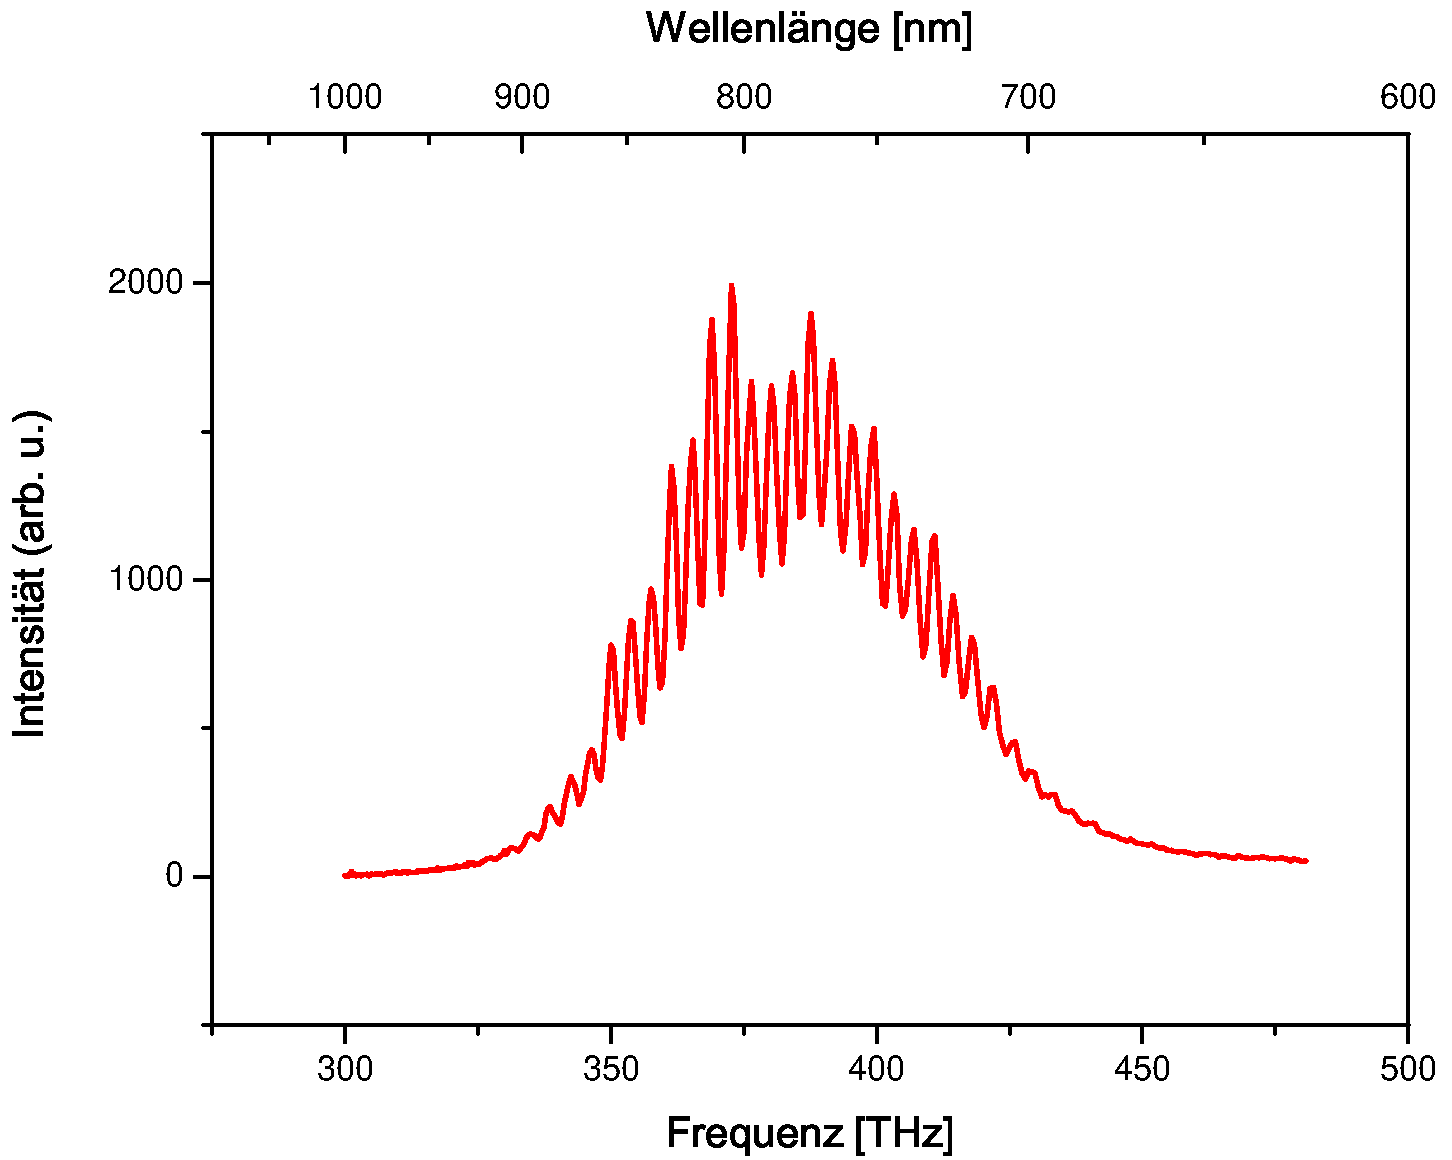
\includegraphics[width=0.49\textwidth]{figures/gratingEtalon}}
   \hfill
   \subfloat[Oszilloskop\label{fig:osziEtalon}]
   {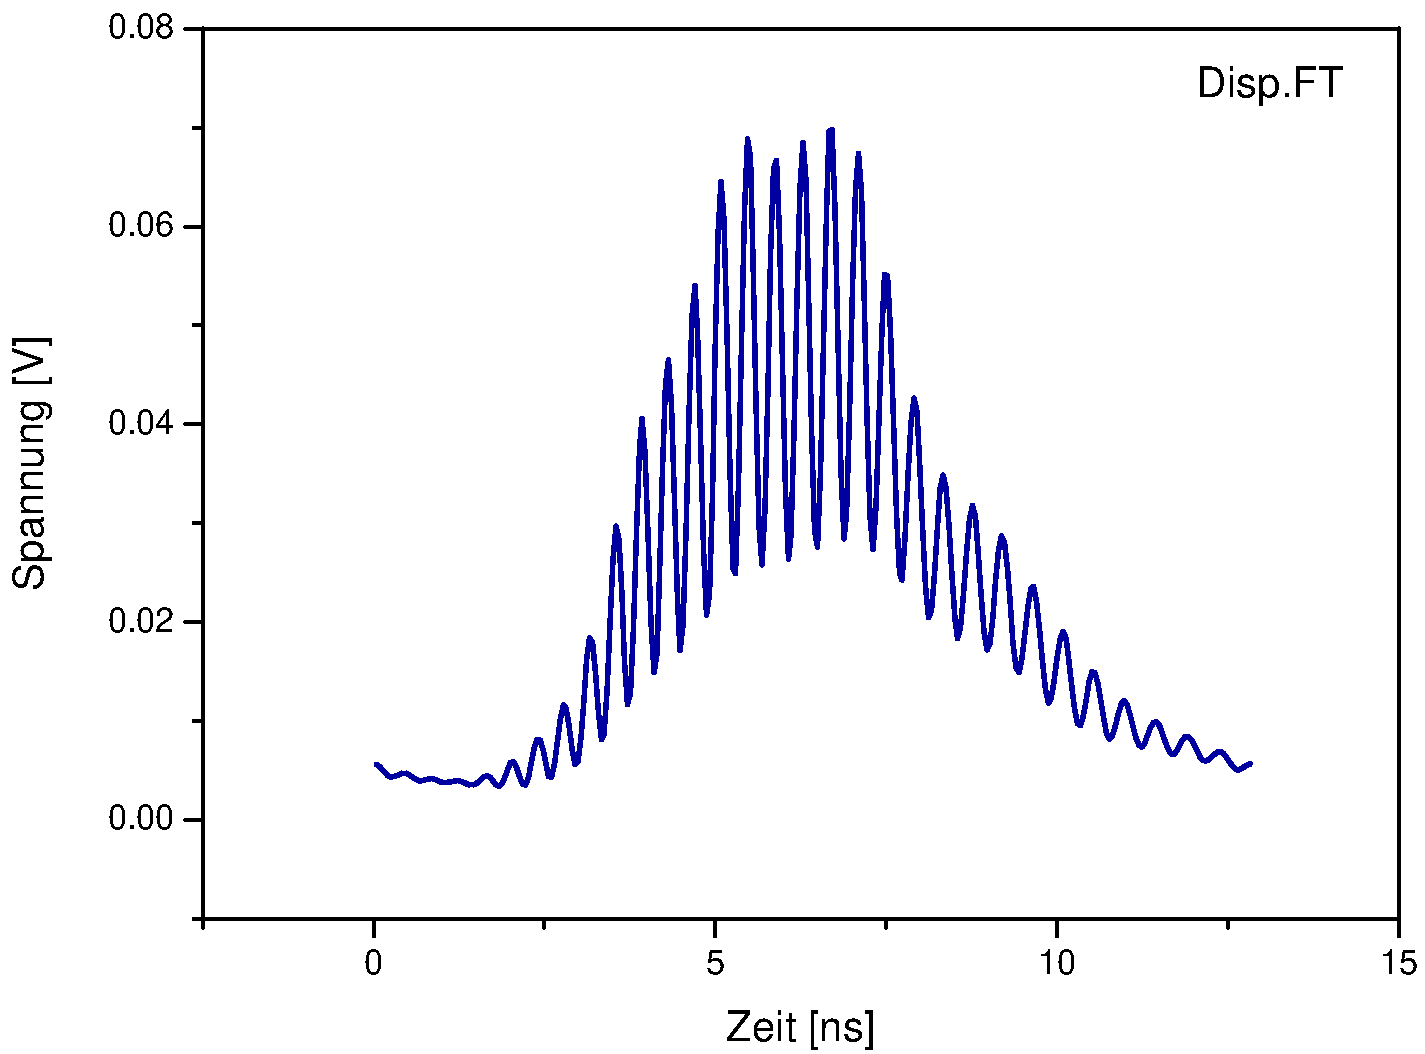
\includegraphics[width=0.49\textwidth]{figures/osziEtalon}}
   \hfill
   \subfloat[Kalibration\label{fig:calibration}]
   {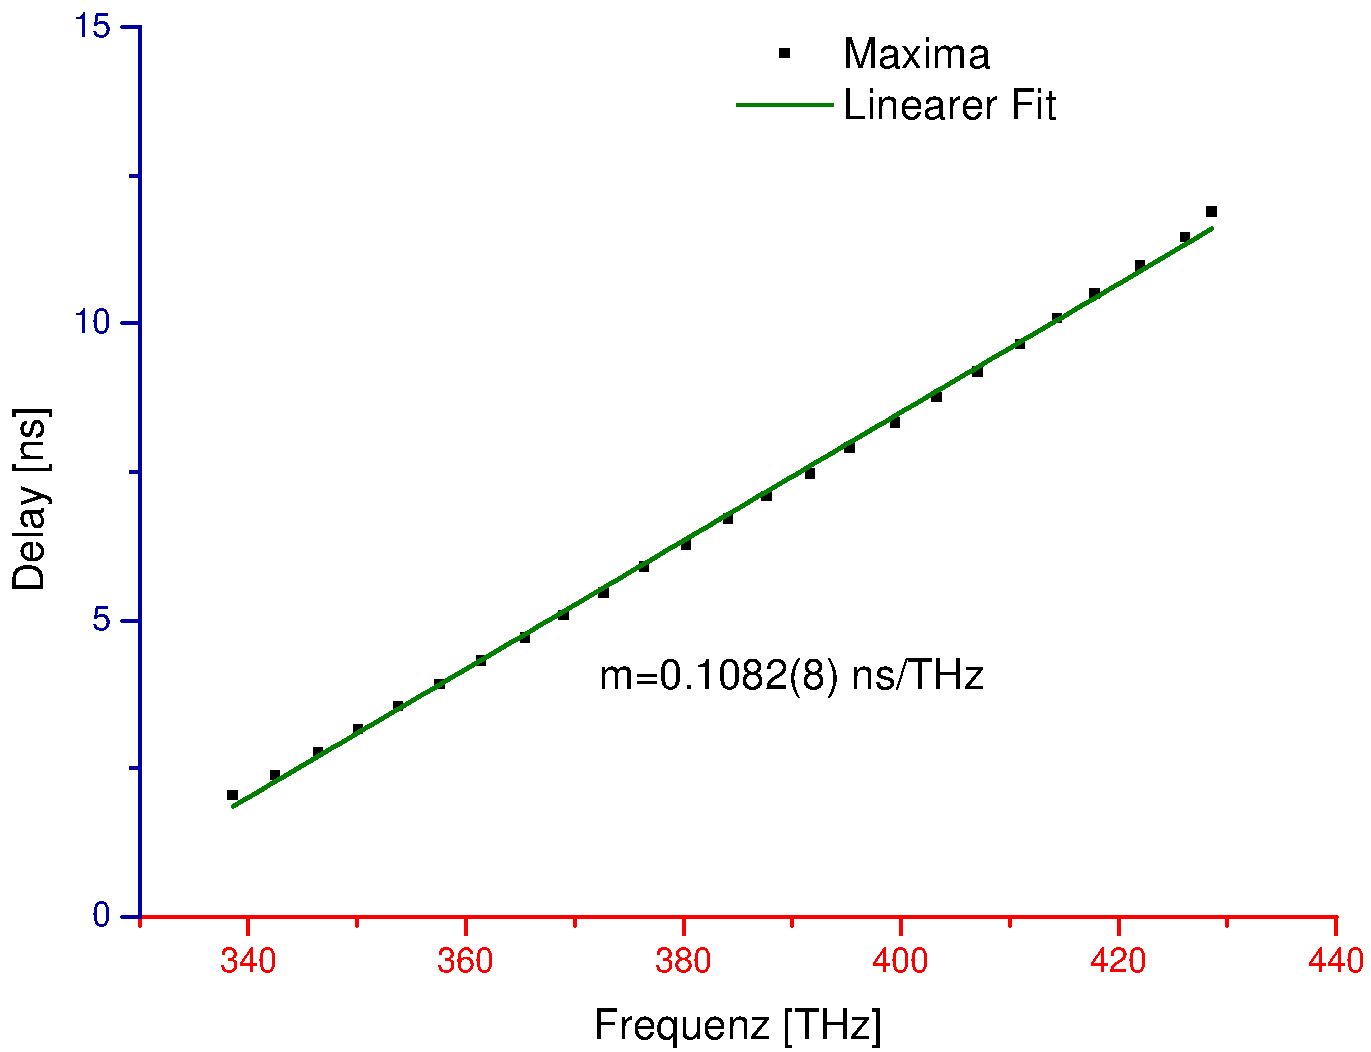
\includegraphics[width=0.6\textwidth]{figures/calibration}}
   \caption{Kalibration durch ein Etalon: Verzögerung nach der Faser wird Frequenzen zugeordnet.}
   \label{fig:caliEtalon}
 \end{figure}

\section{Charakterisierung der Photodioden}
Als nächstes wird die Photodiode (Alphalas UPD-40-UVIR-P) charakterisiert.
In Tabelle \ref{tab:PD} finden sich die wichtigsten Herstellerangaben zu diesem ultraschnellen Photodetektor.
Diese sollen überprüft bzw. auf die experimentelle Situation hin getestet werden.
Die beiden verwendeten Photodioden werden anhand ihrer Seriennummern \texttt{04336} und \texttt{04346} unterschieden.

Zunächst wird getestet, in welchem Leistungsbereich die Photodioden linear reagieren, damit bei zukünftigen Messungen dieser Bereich nicht überschritten wird.
Dies geschieht für die beiden Messmodi mit undispergiertem sowie dispergiertem Signal.
Außerdem wird die Bandbreite der Photodiode bestimmt, denn für die Beobachtung von bis zu 1\,ps entfernten Pulsen ist es wichtig, dass die Photodiode schnell reagiert.
Diese Pulse sind zu nah, um sie im zeitlichen Signal zu unterscheiden.
So können sie nur als spektrale Interferenz detektiert werden.
Um die Leistungsabhängigkeiten zu messen, wird der Laserstrahl mit der $\lambda/2$-Platte variabel abgeschwächt und mit einem Powermeter direkt vor der entsprechenden Photodiode gemessen.

\begin{table}[!htb]
	\centering
	\begin{tabular}{|c|c|}
		\hline
		PD. Spezifikation & Wert \\		
		\hline
		Risetime & < 40\,ps \\
		Bandbreite & >8.5\,GHz \\
		Spektraler Bereich & 350-1700\,nm \\
		Sensitivität @ 800\,nm & 0.12\,A/W\\
		\hline	
	\end{tabular}
	\caption{Herstellerangaben zur Photodiode Alphalas UPD-40-UVIR.}
	\label{tab:PD}
\end{table}

\subsection{Antwortverhalten auf das dispergierte Signal}
Als nächstes treffen Nanosekundenpulse auf die Photodiode, die sich durch die Dispersion in der Faser aus Femtosekundenpulsen ergeben.
Das Signal ähnelt also einem kontinuierlichen Signal.
So wächst bis ca. 10\,mW die Photodiodenantwort linear mit der eingestrahlten Leistung an.
Danach wird die Photodiode übersteuert, sodass nicht genug Ladungsträger zwischen zwei Pulsen nachfließen können, wobei sich die Pulsform stark ändert.
Im linearen Bereich kann allerdings die Sensitivität der Photodiode bestimmt werden.
Diese gibt an, welcher Strom bei einer bestimmten eingestrahlten Leistung von der Photodiode produziert wird.
Um den geflossenen Strom zu erhalten, wird die am Oszilloskop anliegende Spannung durch den benutzen Widerstand von $50\,\si\ohm$ geteilt.
Außerdem wird der Strom noch über einen Roundtrip gemittelt, denn die eingestrahlte Leistung ist nur als Mittlung messbar.
In Abb. \ref{fig:PDdispMeanA} wird all dies für beide Photodioden bestimmt und beide liefern sehr ähnliche Sensitivitäten: 0.1154(8)\,A/W für  \texttt{04336} und  0.1120(5) für \texttt{04346}.
Der kleine Unterschied kann auch durch eine leicht unterschiedliche Fokussierung bedingt sein.
Insgesamt sind beide Werte aber in gutem Einklang mit der aus dem Datenblatt\footnote{\url{http://www.alphalas.com/images/stories/products/laser_diagnostic_tools/Ultrafast_Photodetectors_UPD_ALPHALAS.pdf}, abgerufen am 08.02.2016} entnommenen Sensitvitätskurve in Abb.\ref{fig:PDsensDB}

\begin{figure}[!htb]
	\centering
	\subfloat[Der mittlere Stromfluss skaliert linear mit der eingestrahlten Leistung.
	Die Steigung entspricht der Sensitivität.\label{fig:PDdispMeanA}]
   {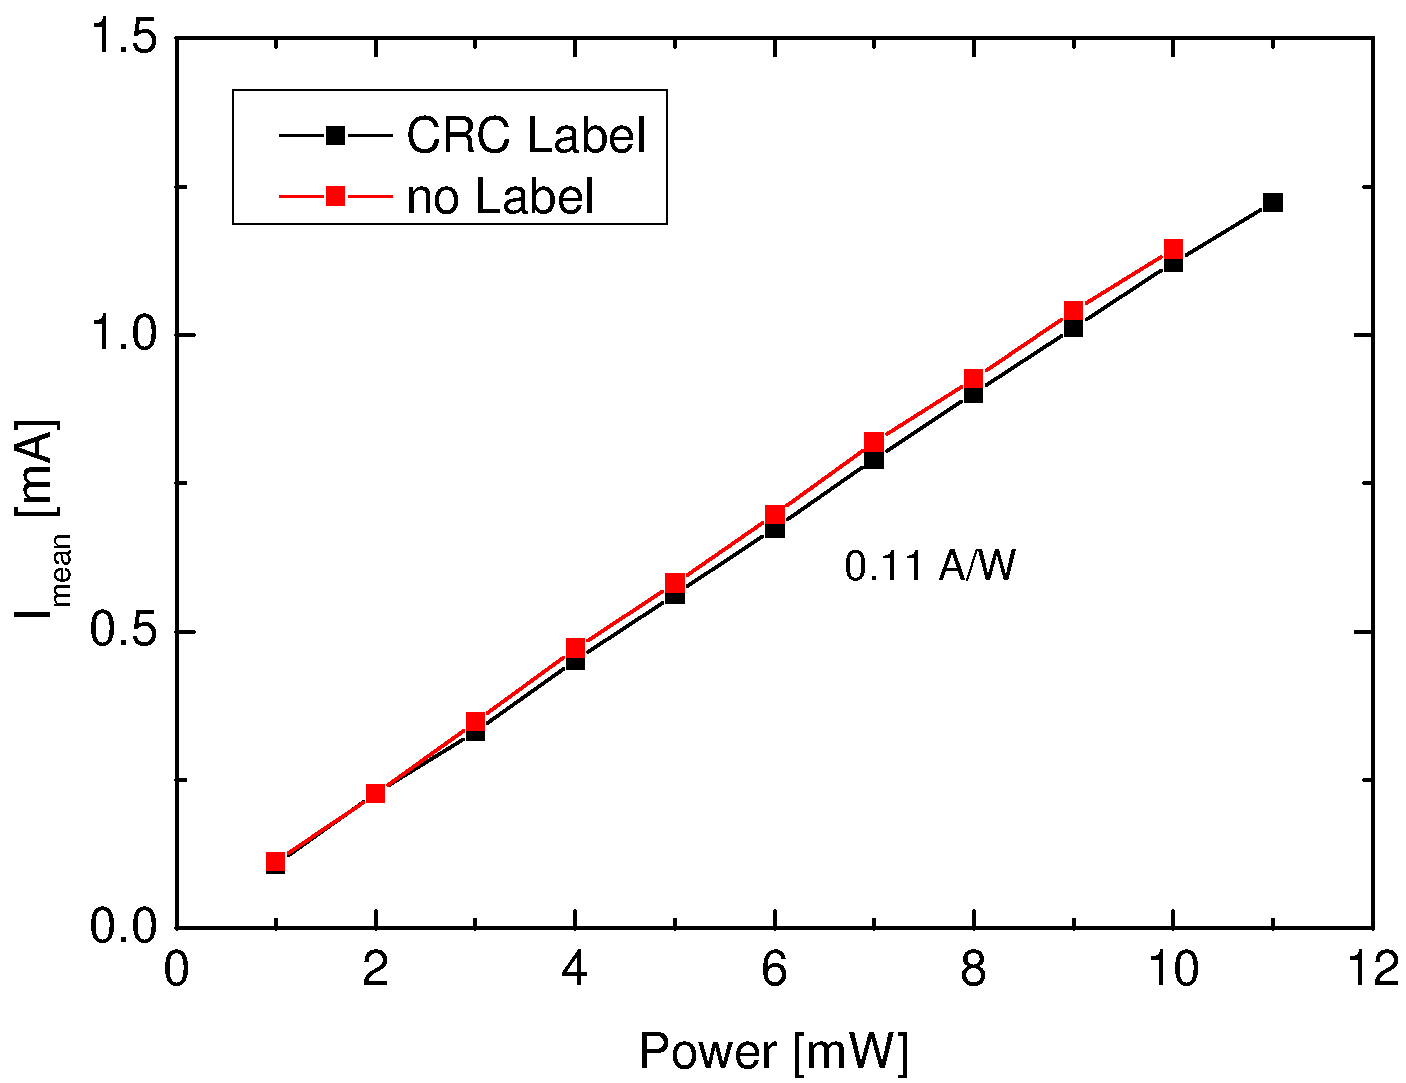
\includegraphics[scale=0.29]{figures/PDdispMeanA}}
   \hfill
   \subfloat[Wellenlängenabhängige Sensitivität aus dem Datenblatt im Vergleich mit dem gemessenen Wert und dem Pulsspektrum nach der dispersiven Faser.\label{fig:PDsensDB}]
   {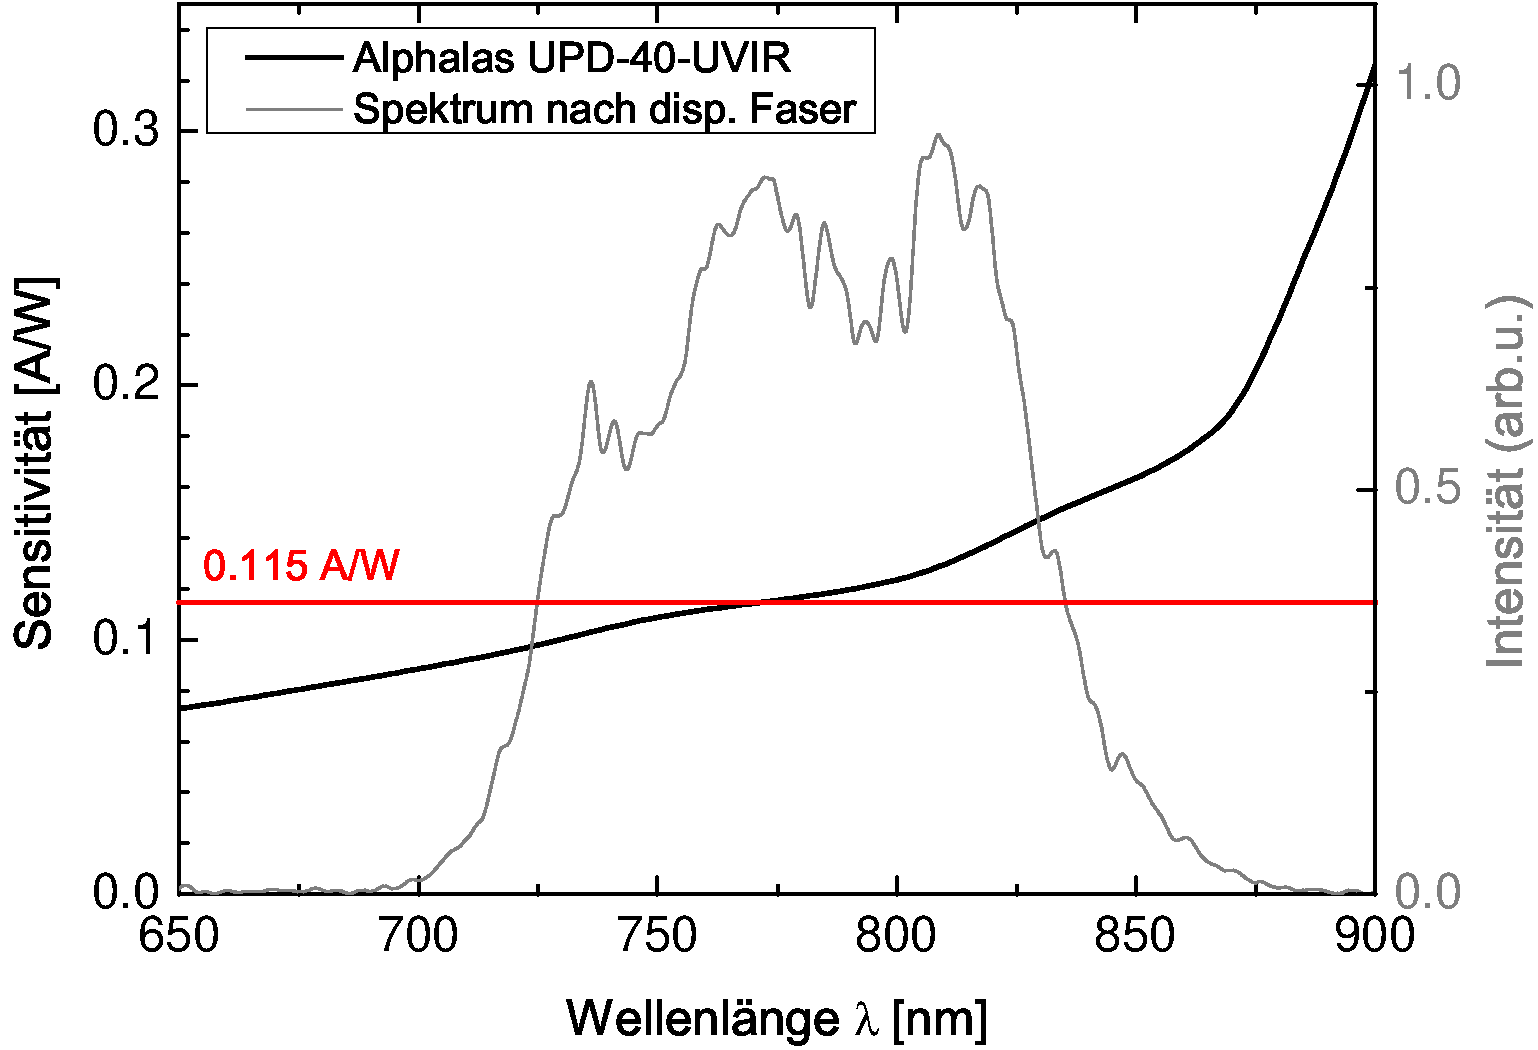
\includegraphics[scale=0.29]{figures/PDsensitivty}}
	\caption{Sensitivität der Photodioden.}
	\label{fig:PDsens}
\end{figure}

\subsection{Antwortverhalten auf das undispergierte Signal}
In Abbildung \ref{fig:PDfwhmMaxI} ist in Abhängigkeit der eingestrahlten Leistung die Photodiodenantwort auf das undispergierte Signal dargestellt.
Hier ist  das optische Eingangssignal viel kürzer als die Risetime der Photodiode.
Erkennbar ist, dass die Peakamplitude bis ca. 2\,mW linear ansteigt und in dieser Region die Pulslänge (FWHM) etwas über 100\,ps liegt.
Dies entspricht der angegebenen Risetime von 40\,ps.
Um also die besten Ergebnisse zu erzielen, sollte die Photodiode in diesem Betriebsmodus nicht mit mehr als 2\,mW bestrahlt werden.
Je nach Justage ist ein Ringing nach dem Puls zu beobachten (vgl. Abb.\ref{fig:PD2mW}).

Auffällig ist, dass die Halbwertsbreite sowie die Peakspannung für die Diode mit der Seriennummer \texttt{04346} schneller anwächst.
Dies würde auf eine höhere Sensitivität hindeuten.
Im obigen Abschnitt werden aber ähnliche Sensitivitäten für beide Photodioden gemessen.
So ist der Unterschied wahrscheinlich auf ungleiche Bestrahlungsverhältnisse zurückzuführen.
Dies wird auch durch den Unterschied in der Sättigungsspannung untermauert.
Eventuell war bei Messung von \texttt{04336} die Linse vor der Photodiode nicht so positioniert, dass der Laserstrahl nur auf den sensitivsten Bereich der Photodiode trifft.
\clearpage
\begin{figure}[!htb]
	\centering
	\subfloat[Antwortverhalten der beiden Photodioden: Bei steigender Leistung sättigt die Peakspannung und die Photodioden-Antwort wird länger.\label{fig:PDfwhmMaxI}]
   {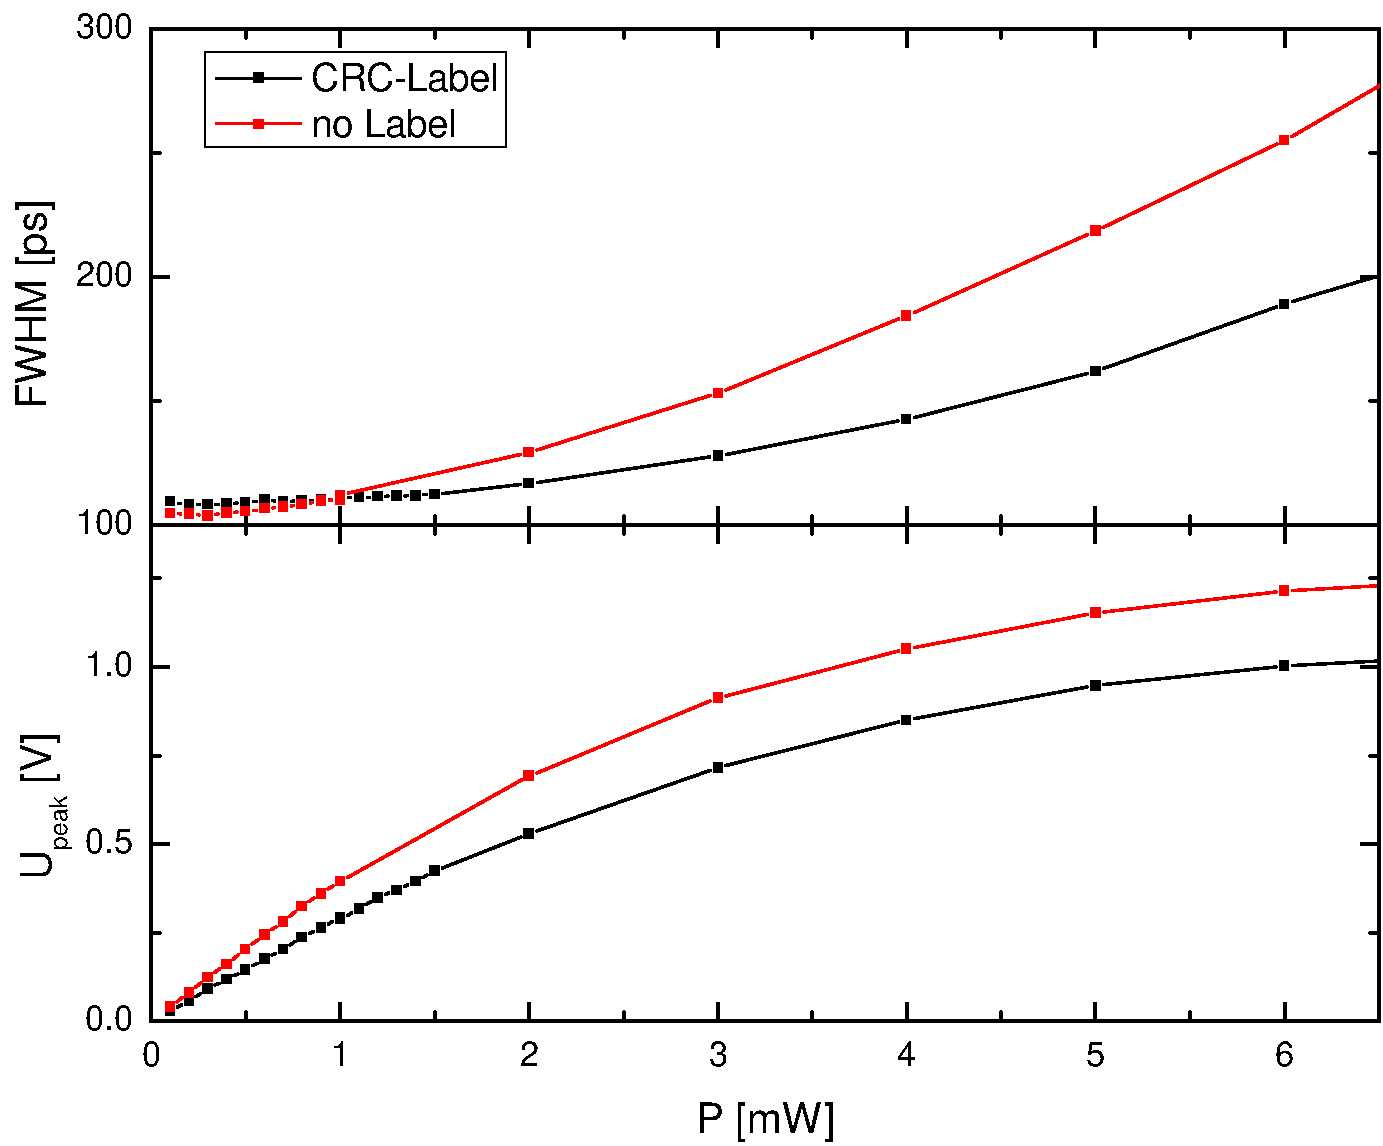
\includegraphics[width=0.49\textwidth]{figures/PDfwhmMaxI}}
   \hfill
   \subfloat[Vergleich der beiden Dioden bei 2\,mW: Unterschied kann auch auf Einstrahlung zurückzuführen sein. \label{fig:PD2mW}]
   {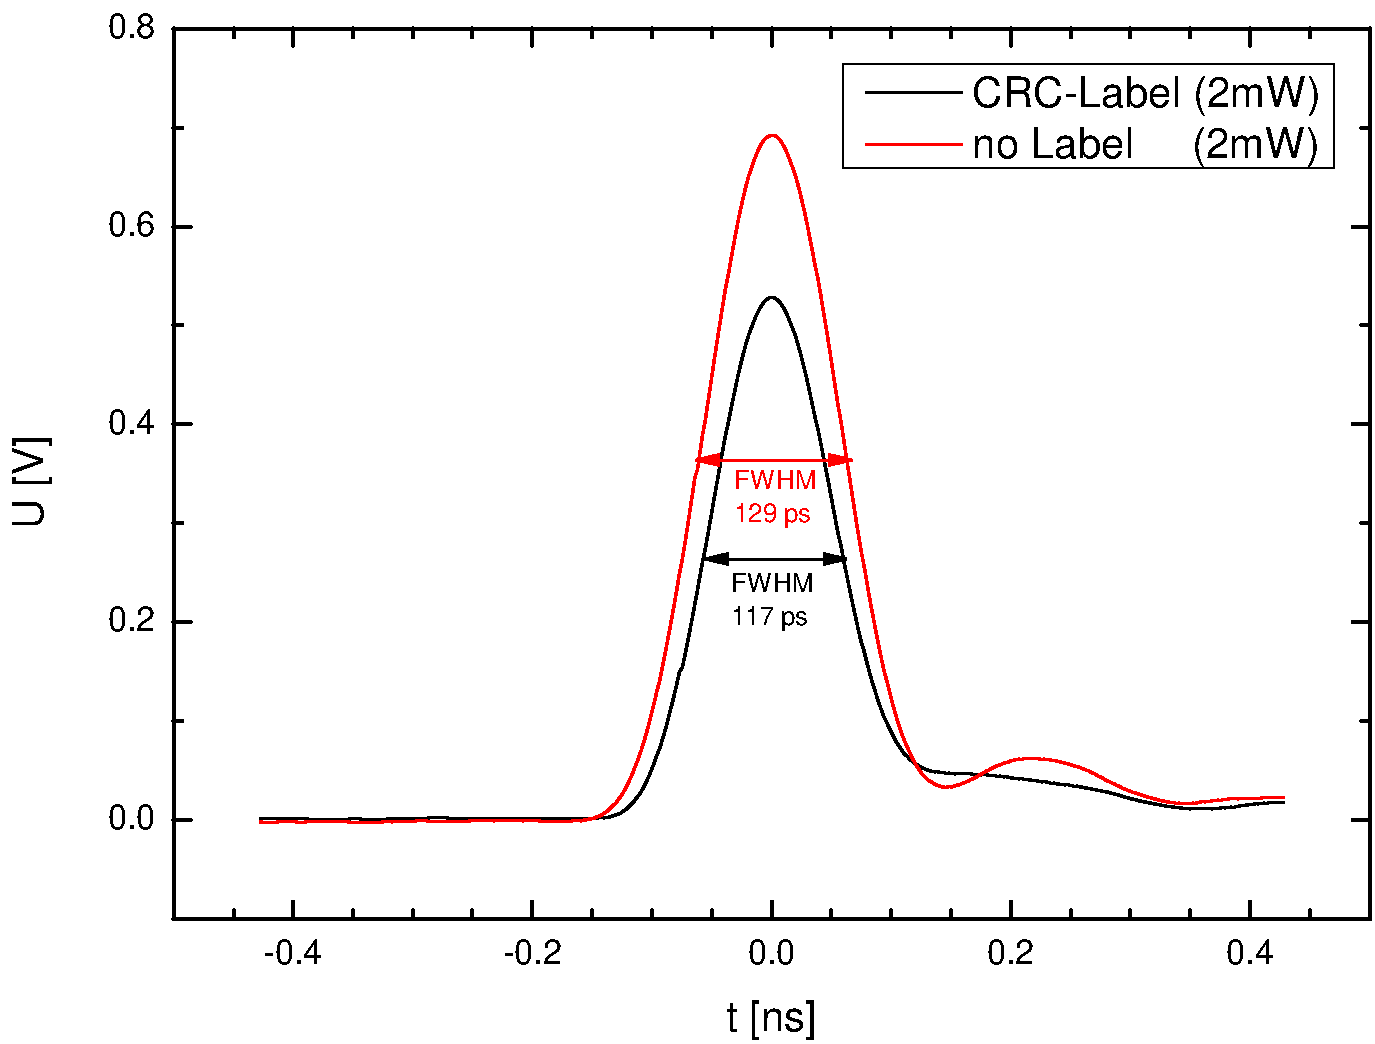
\includegraphics[width=0.49\textwidth]{figures/PD2mW}}
	\caption{Photodiodenantwort auf undispergiertes Signal.}
	\label{fig:PDundisp}
\end{figure}

\subsection{Bandbreite der Photodiode}
Das Spektrum sollte voll durchmoduliert sein, wenn beide Pulse gleich stark sind.
Die Photodiode wird jedoch ab einer bestimmten Modulationfrequenz, also einem bestimmten Abstand der Doppelpulse, nicht so schnell reagieren können.
Daher reduziert sich die Modulationstiefe für hohe Frequenzen.
Dadurch kann der Intensitätsunterschied der beiden Pulse überschätzt werden.
Um dies zu untersuchen, wird ein Michelson-Interferometer in den Strahlengang eingebaut (vgl. Abb.\ref{fig:Beamsplitter}).
Mit diesem können durch Variation einer Armlänge Pulspaare mit veränderlichem Abstand hergestellt werden.
Diese Abstände finden sich in der Modulation des Spektrums wieder.
Mit einem Powermeter wird außerdem verifiziert, dass beide Pulse die gleiche Energie haben.

\begin{figure}[!htb]
	\centering
	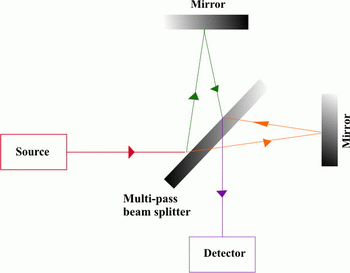
\includegraphics[width=0.55\textwidth]{figures/multi_pass_beam_splitter.png}
	\caption{Schematische Zeichnung eines Michelson-Interferometers\protect\footnotemark:
	Bei beiden Armen wird der Strahl jeweils einmal reflektiert sowie einmal transmittiert, sodass die zwei Strahlengänge die gleiche Leistung aufweisen.
	Die Reflexion an der Vorderkante des Strahlteilers führt jedoch zu verschiedenen Propagationslängen im Glas des Strahlteilers und somit zu etwas höherer Dispersion im Arm des zuerst transmittierten Strahls.}
	\label{fig:Beamsplitter}
\end{figure}
\footnotetext{\url{http://www.tydexoptics.com/images/products/multi_pass_beam_splitter.gif}, abgerufen am 14.08.2016}

Aufgrund der Funktionsweise des verwendeten Strahlteilers findet die Reflexion nur an der Vorderseite statt (vgl. Abb.\ref{fig:Beamsplitter}).
Dies führt dazu, dass der zuerst reflektierte Strahl einmal, aber der zuerst transmittierte Strahl zweimal den Strahlteiler passiert.
Dieser sorgt für einen positiven Chirp der Pulse, dh. die niedrigen Frequenzen laufen den hohen Frequenzen voraus.
Da der zuerst transmittierte Puls jedoch stärker gechirpt wird, ist der Pulsabstand   hinter dem Interferometer frequenzabhängig: Ist der stärker gechirpte Puls vor dem anderen, dann haben die niedrigeren Frequenzen einen größeren Abstand als die höheren. Ist die Pulsreihenfolge umgekehrt, so haben die niedrigeren Frequenzen einen kleineren Abstand.
Die resultierende Modulationsfrequenz im Spektrum ist also nicht konstant.
Mit einer entsprechenden Kompensationsplatte in einem der beiden Arme kann dies verhindert werden, hier wird dieser Chirp jedoch genutzt:
So kann dieser die Abweichung von einem linearen Zusammenhang zwischen Frequenz und deren zeitlicher Verzögerung nach der Faser kompensieren oder verstärken.
In Abbildung \ref{fig:calibration} ist nämlich zu erkennen, dass ein bestimmter Frequenzabstand bei niedrigen Frequenzen einen geringeren zeitlichen Abstand aufweist als bei höheren Frequenzen.
Ist der Pulsabstand für niedrige Frequenzen geringer, haben die Frequenzen konstruktiver Interferenz einen größeren Abstand im Spektrum, der dann durch die Faser kompensiert wird, sodass das Signal nach der Faser nur eine bestimmte Modulationsfrequenz aufweist.
Dies ist für die Charakterisierung der frequenzabhängigen Antwort der Photodiode nötig.
Diese könnte man mit einem kontinuierlich modulierten Signal besser messen, benötigt dazu jedoch einen Modulator im 10\,GHz-Bereich.

\begin{figure}[!htb]
   \centering
   \subfloat[Spektrum als Signal nach der Faser in Abhängigkeit der Armlängendifferenz.]
   {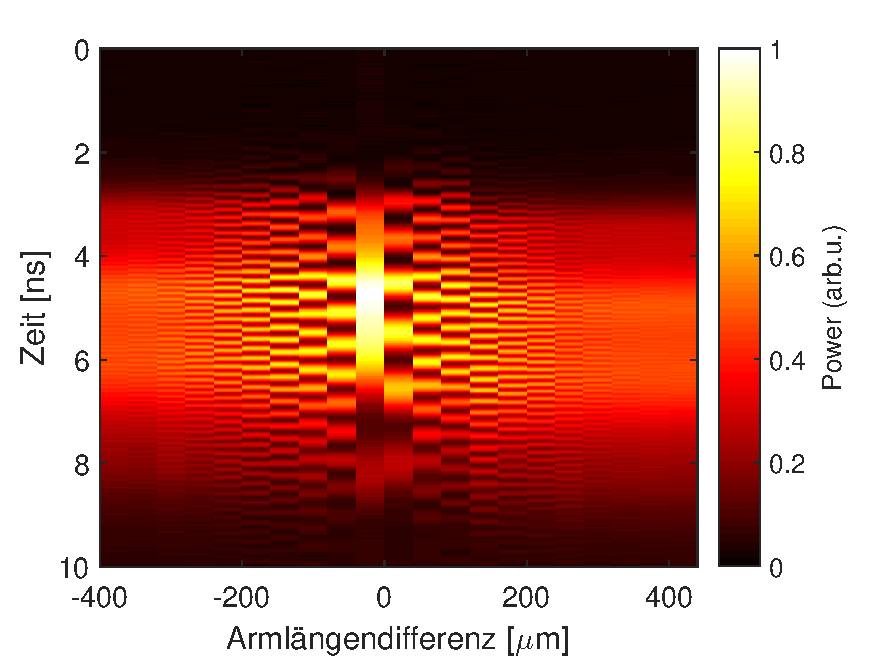
\includegraphics[width=0.49\textwidth]{figures/PDBandbreite_DATA}}
   \hfill
   \subfloat[Fouriertransformierte von a) logarithmiert \label{fig:PDBandbreite_FFT}]
   {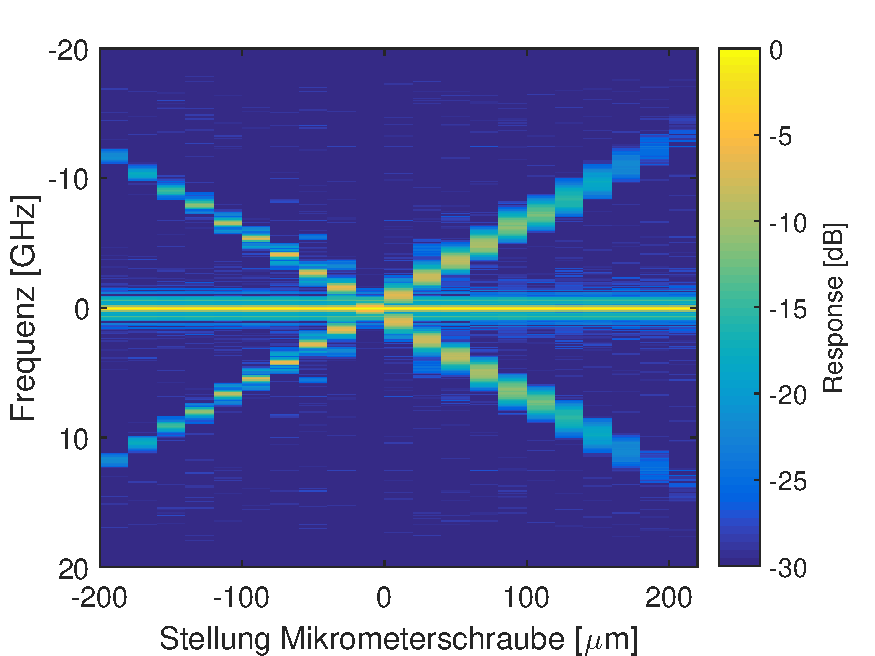
\includegraphics[width=0.49\textwidth]{figures/PDBandbreite_FFT}}
   \caption{Bandbreitenbestimmung der Photodiode durch ein Interferometer: Die Variation des Pulsabstandes ermöglicht verschiedene Modulationsfrequenzen des Signals nach der Faser (Doppelpulsspektren) und somit die Charakterisierung der Photodiode.}
   \label{fig:PDBandbreite}
\end{figure}

\begin{figure}[!htb]
	\centering
	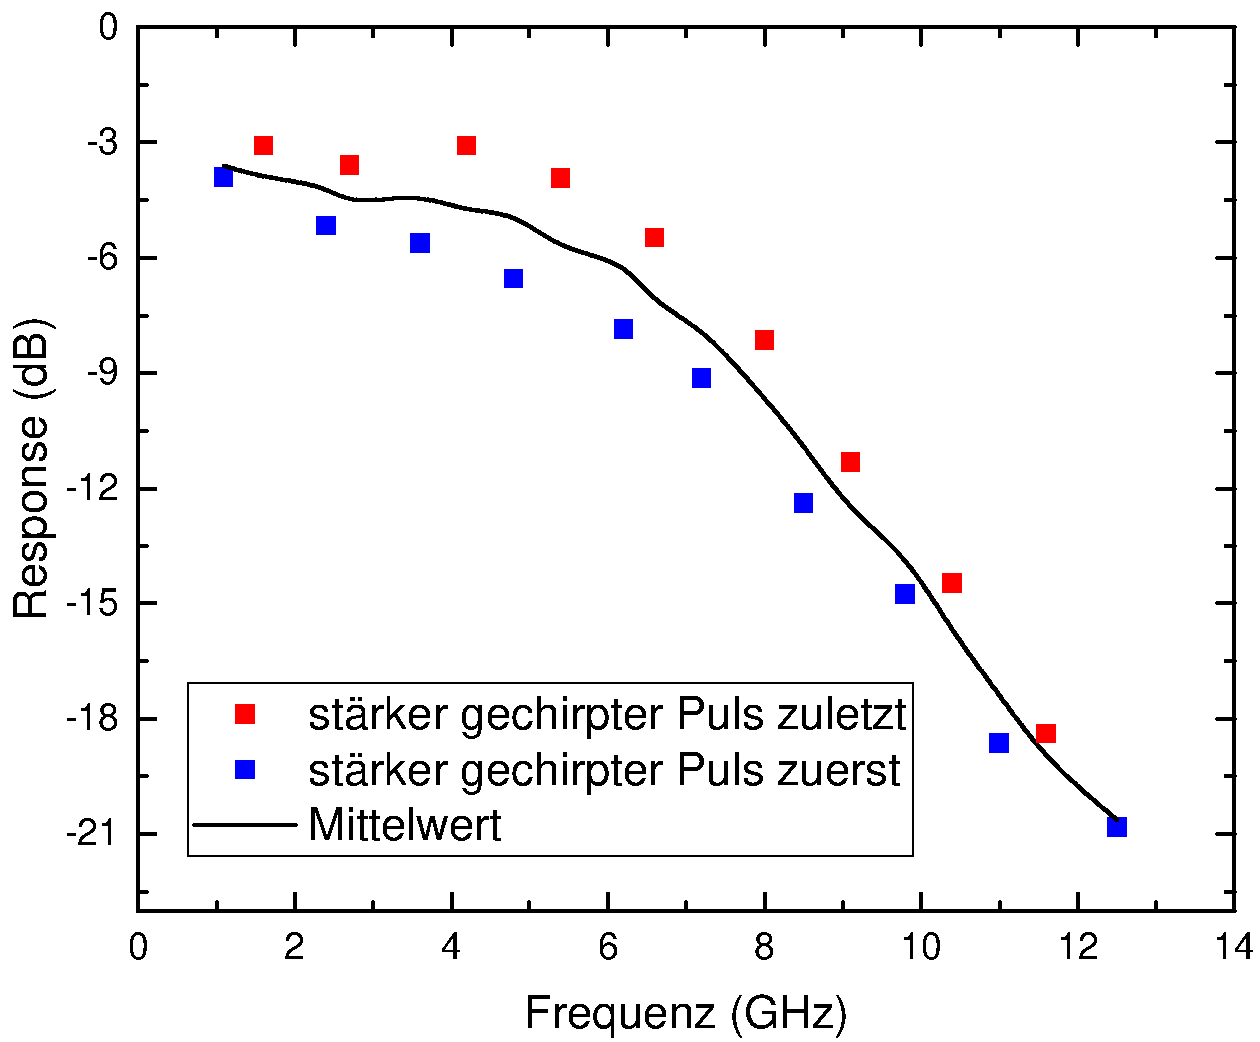
\includegraphics[width=0.7\textwidth]{figures/PDBandwidth}
	\caption{Relative Höhe der Nebenmaxima in Abhängigkeit der jeweiligen Modulationsfrequenz aus Abb.\ref{fig:PDBandbreite_FFT}.}
	\label{fig:PDBandbreiteAusw}
\end{figure}

\chapter{Ergebnisse}
In diesem Kapitel wird zunächst erläutert, wie der Resonator justiert sein muss, um Multipulse erzeugen zu können.
Danach wird erklärt, wie die Messdaten bearbeitet werden, damit man aus ihnen Pulsabstände bestimmen kann.
Mit diesem Vorwissen werden dann die beobachteten Multipulse dargestellt.
Dabei wird sich hier auf Multipulse mit geringen Pulsabständen ($< 1\,$ps) beschränkt.
Wie schon von \cite{lai_multiple_1997} beschrieben, gibt es aber auch Multipulszustände mit langen Abständen.
Im Abschnitt \ref{sec:cpml} wird auf diese und deren Interaktionsmechanismus genauer eingegangen.

\section{Kartierung des Resonators}
Für das Einstellen von Multipulsen ist die Kenntnis der wichtigsten Resonatorparameter nötig.
Dazu gehört die Kristallposition und der Abstand zwischen den beiden fokussierenden Spiegeln.
Diese Abstände können jedoch aufgrund der Gegebenheiten momentan nur mit einer Genauigkeit von ca. $20\,\si{\micro\meter}$ gemessen werden.

In Abbildung \ref{fig:map} wird der Abstand der fokussierenden Spiegel bei verschiedenen Kristallpositionen variiert.
In Abhängigkeit dessen wird mit einem Powermeter direkt am Laserausgang die cw-Leistung und -- wenn möglich -- auch die gemodelockte Leistung gemessen.
Zu erkennen ist, dass die cw-Leistung geringer wird, wenn der Abstand zwischen den beiden Spiegeln verringert wird.
Dies entspricht dem typischen Verlauf, den Laser zu justieren:
Zuerst wird die cw-Leistung durch Justage der Resonator-Endspiegel bei weitem Abstand maximiert.
Danach wird der Abstand der beiden Fokussierspiegel verringert, während der Endspiegel schnell bewegt wird, um Fluktuationen zu erzeugen, die bei geeigneter Stellung den modengekoppelten Betrieb erzeugen.
Die Ausgangsleistung ist im modengekoppelten Betrieb größer als die cw-Leistung und nahezu unabhängig von der Stabilitätsposition.
Somit nimmt der Leistungsunterschied zwischen den beiden Betriebsmodi zu größeren Stabilitätspositionen (kleineren Spiegelabständen) zu.
Der modengekoppelte Puls wird unempfindlicher auf Störungen.
Die Kristallposition beeinflusst auch die Leistung: Zum einen gibt es eine Position maximaler Leistung.
Zum anderen ist zu erkennen, dass eine größere Kristallposition (kleinerer Abstand zwischen Kristall und fixem Fokussierspiegel) zu einer Aufspaltung des modelockbaren Bereiches führt.

\begin{figure}[!htb]
	\centering
	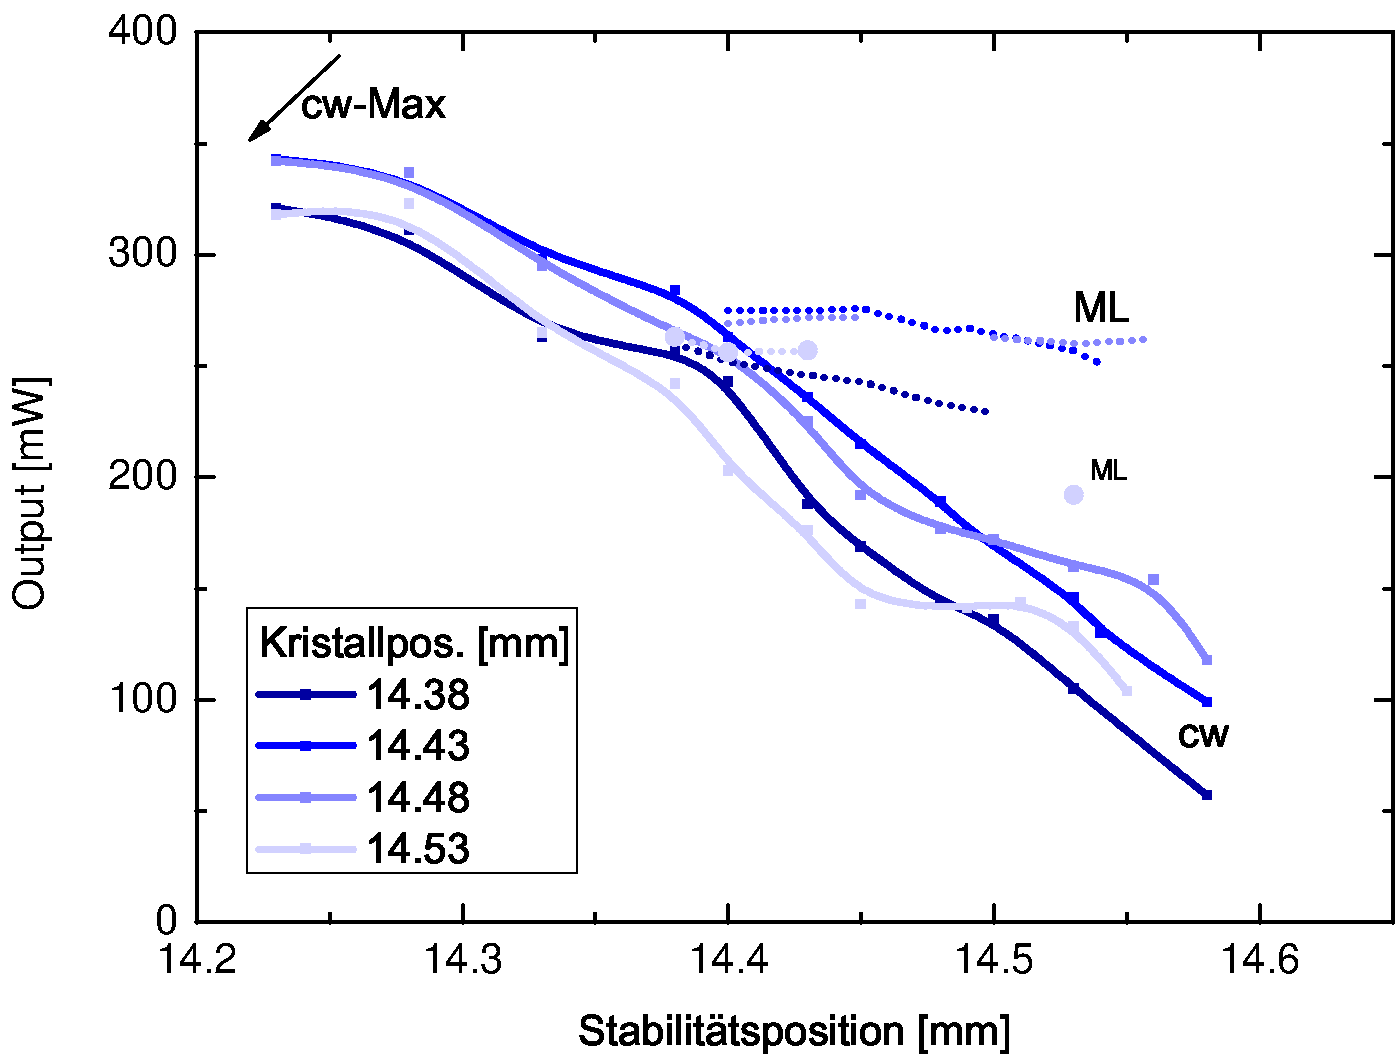
\includegraphics[width=0.7\textwidth]{figures/map.pdf}
	\caption{Abhängigkeit der Leistung (cw \& modengekoppelt) von der Position des fokussierenden Spiegels (Stabilität) bei verschiedenen Kristallpositionen.
	Die Positionen werden von außen gemessen, dh. dass größere Werte einer Verringerung des Abstandes zum festen Fokussierspiegel entsprechen.}
	\label{fig:map}
\end{figure}

Bei welchen Justagen lassen sich Multipulse erzeugen?
In Abbildung \ref{fig:map2} wird die Leistungsabhängigkeit von der Stabilitätsposition bei fester Kristallposition sowohl im cw-Betrieb als auch im Einzel-/Doppelpuls-Zustand  dargestellt.
Wieder ist das gleiche Verhalten für den cw-Fall (schwarz) zu erkennen.
Die Einzelpuls-Leistung (rot) ist etwas größer, die Doppelpuls-Leistung (blau) noch größer.
Zu beachten ist aber, dass die Leistung im Doppelpulsbetrieb nicht annähernd doppelt so groß ist wie die Einzelpuls-Leistung.
Also sind die beiden Pulse des Paares jeweils nicht so energiereich (und wahrscheinlich nicht so kurz) wie der Puls im Einzelpulsbetrieb.
Vom Einzelpulsbetrieb ausgehend, können Doppelpulse durch Verringerung der Stabilitätsposition eingestellt werden.
Meist befindet sich der Laser nach der ersten Störung durch Bewegen des Endspiegels  im Einzelpuls-Zustand.
Das Spektrum dieses Zustands ist aber mit einem hohen cw-Anteil behaftet.
Die gesamte Ausgangsleistung ist also nicht in diesem Puls vereint.
Wird der Laser durch Bewegen des Endspiegels ein zweites Mal gestört, können sich Doppelpulse einstellen.

\begin{figure}[!htb]
	\centering
	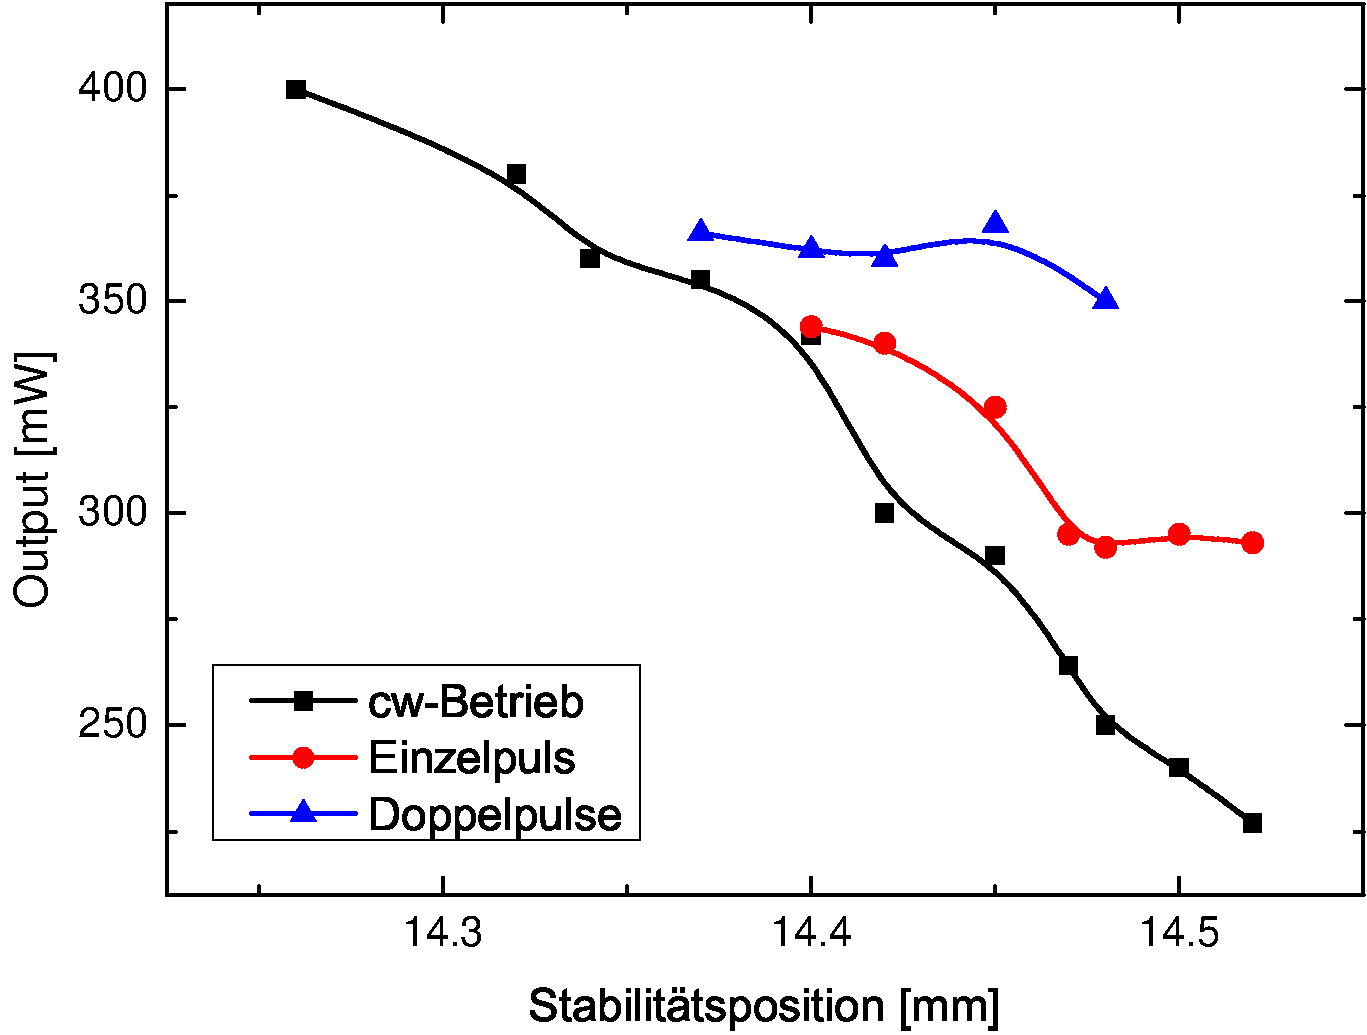
\includegraphics[width=0.7\textwidth]{figures/map2.pdf}
	\caption{Abhängigkeit der Ausgangsleistung (cw \& modengekoppelt) von der Position des fokussierenden Spiegels (Stabilität) bei fester Kristallposition.}
	\label{fig:map2}
\end{figure}


\section{Darstellung der Messdaten}
Um durch eine lange Messung mit dem Oszilloskop die Entwicklung des Spektrums darstellen zu können, muss zunächst die Pulswiederholrate bestimmt werden.
Dies geschieht über eine Fouriertransformation des gesamten Signals.
Die Frequenz des höchsten Peaks entspricht der Wiederholrate, das Inverse also dem Pulsabstand $t_\text{rep}$ bzw. der optischen Resonatorlänge des Lasers.
Da sich diese zum Starten ändert, ist die bestimmte Wiederholrate nur für einen kurzen Ausschnitt der Messung korrekt.
Ist also $t_\text{rep}$ bestimmt, wird festgelegt, in wie viele äquidistante Punkte diese Zeit unterteilt werden soll.
Dies sollte so gewählt sein, dass die Abstände in etwa zugehörigen Samplingrate entspricht.
Dann werden die Messdaten an den neuen Zeitpunkten interpoliert und anschließend als 2D-Matrix dargestellt, man trennt also jeden Roundtrip.
Die eine Dimension entspricht den Roundtrips, die andere entspricht der schnellen Zeitachse.

Zuletzt muss noch die Änderung der Repetitionsrate bzw. die Abweichung vom richtigen Wert korrigiert werden.
Dies kann auf zwei Arten geschehen:
Dazu wird ein Polynom durch die Peakpositionen des undispergierten, gemodelockten Signals gelegt. Der Definitionsbereichs des Polynoms wird auf die gesamte Messung ausgedehnt und dann wird jeder Roundtrip so verschoben, dass diese Peakpositionen zu gleichen Zeitpunkten im Roundtrip liegen.
Mit diesem Polynom (evtl. mit anderem Offset) wird auch die dispergierte Messung verschoben.

\begin{figure}[!htb]
   \centering
   \subfloat[Die gemessene Zeitreihe wird in Laserumläufe unterteilt. Diese können dann zu einer 2D-Matrix zusammengesetzt werden -- wie in b) und c) geschehen.
   \label{fig:plainData}]
   {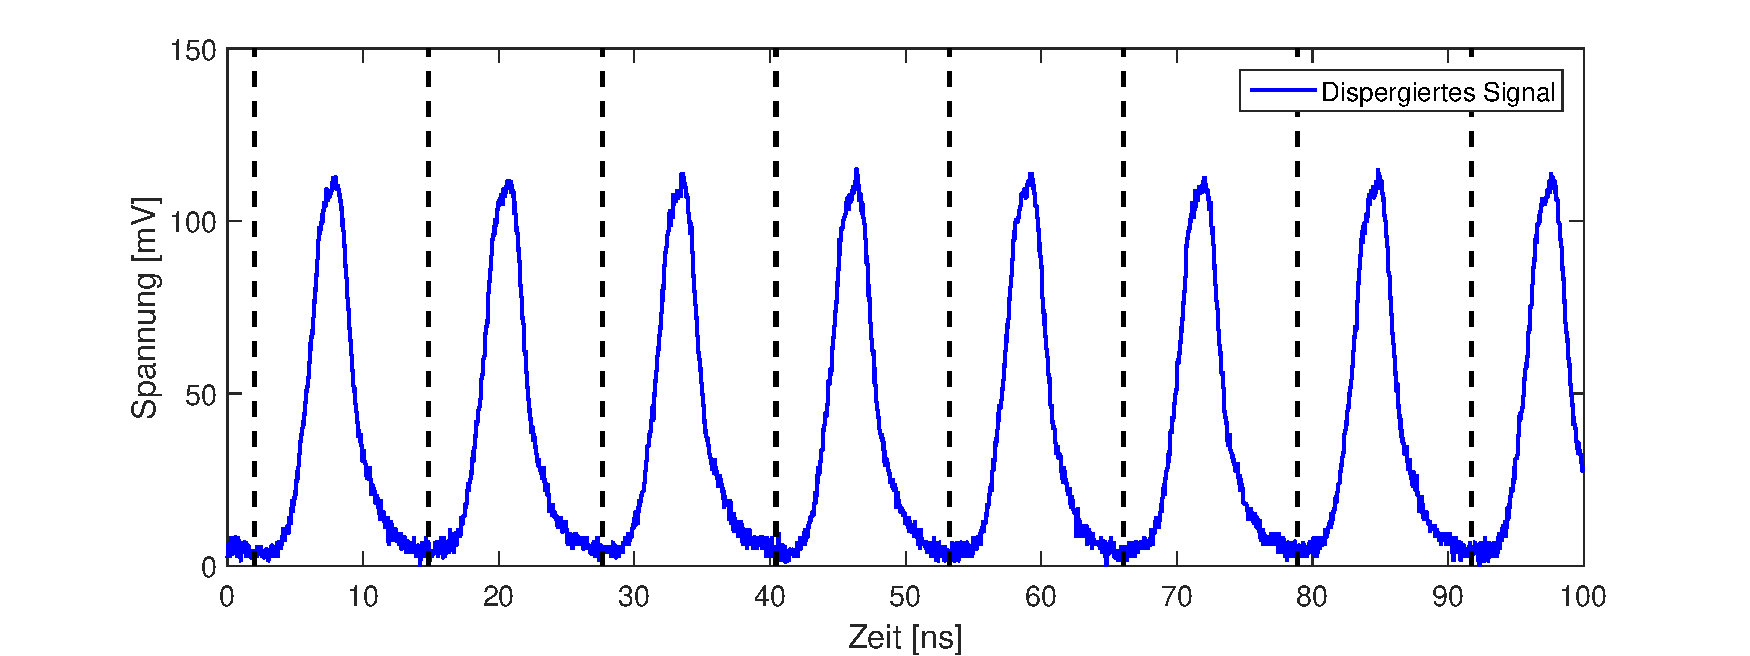
\includegraphics[width=\textwidth]{figures/4ms_25GSA_400m_MLstart_negDisp1_plainDATA.pdf}}
   
   \subfloat[Matrix des undispergierten Signals.\label{fig:rBF463}]
   {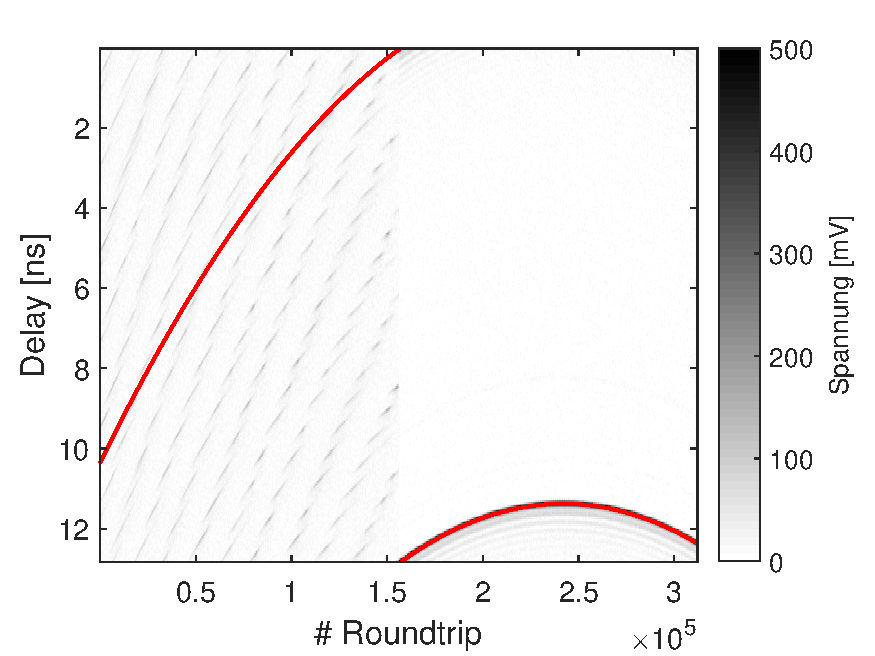
\includegraphics[width=0.5\textwidth]{figures/4ms_25GSA_400m_MLstart_negDisp1_Ch2_krumm.pdf}}
   \hfill
   \subfloat[Matrix des dispergierten Signals.\label{fig:rBF464}]
   {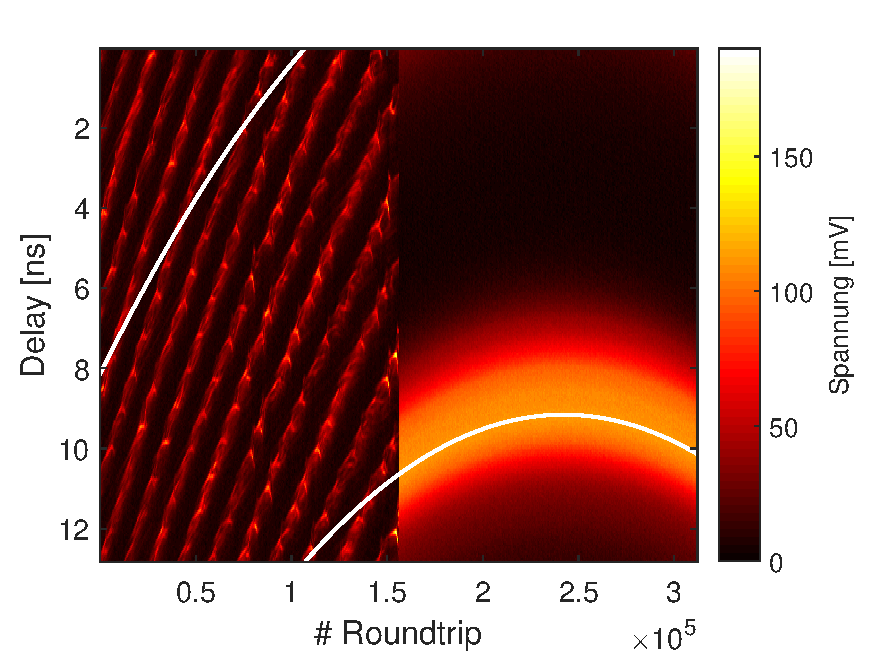
\includegraphics[width=0.5\textwidth]{figures/4ms_25GSA_400m_MLstart_negDisp1_Ch1_krumm.pdf}}
   
   \subfloat[Matrix des undispergierten Signals,\protect\\ Änderung der Repitionsrate korrigiert.\label{fig:rBF463}]
   {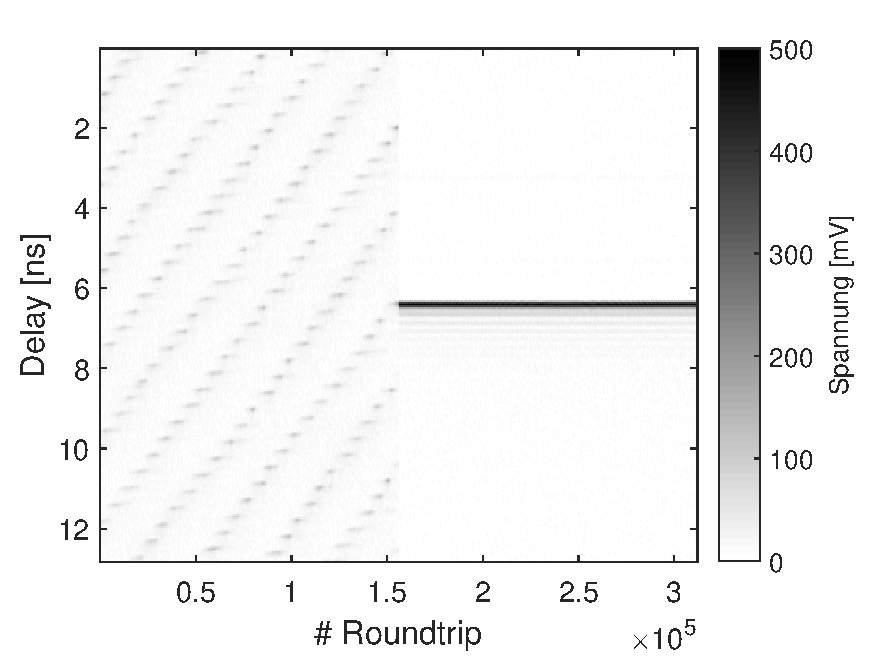
\includegraphics[width=0.5\textwidth]{figures/4ms_25GSA_400m_MLstart_negDisp1_Ch2_glatt.pdf}}
   \hfill
   \subfloat[Matrix des dispergierten Signals,\protect\\ Änderung der Repitionsrate korrigiert.\label{fig:rBF464}]
   {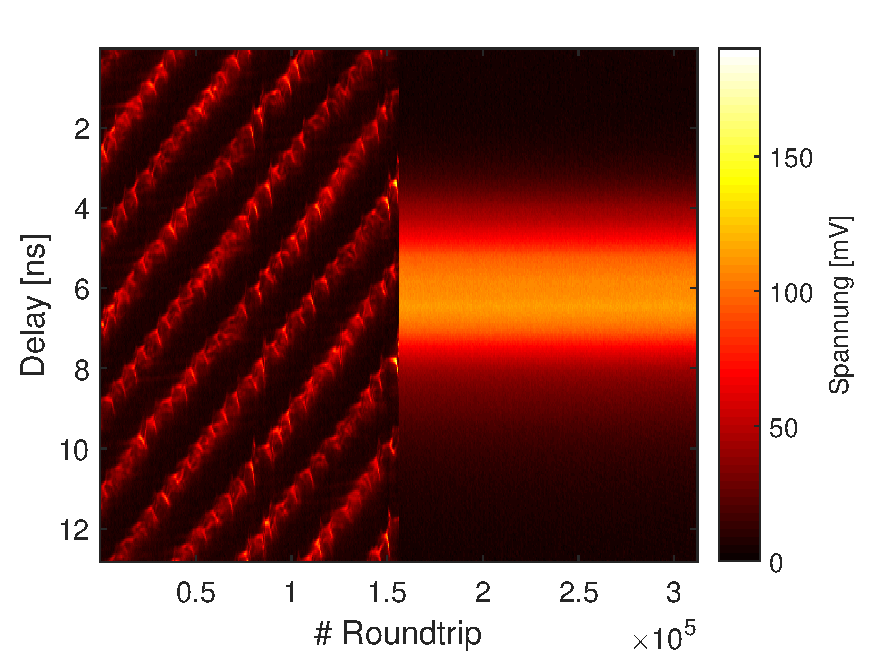
\includegraphics[width=0.5\textwidth]{figures/4ms_25GSA_400m_MLstart_negDisp1_Ch1_glatt.pdf}}
   \caption{Darstellung der Messdaten: Die gemessene Zeitreihe wird in Laserumläufe aufgetrennt, dann wird die Auswirkung der Änderung der Resonatorlänge während der Messung korrigiert.}
   \label{fig:MessdatenDarstellung}
\end{figure}
 


\clearpage
\section{Doppelpulse Messreihe 1}
Wie zuvor beschrieben, wird der Laser bei geeigneter Justage durch zweimaliges Stören in den Doppelpuls-Betrieb überführt.
Durch anschließendes Variieren der Pumpleistung lassen sich drei verschiedene Regime beobachten.
Bei einer hohen Pumpleistung von $P_\text{Pump}=4.57\dots 4.81\,$W sind die Pulse gebunden.
Es lässt sich eine interessante Phasen-Abstandsdynamik beobachten.
Bei einer mittleren Pumpleistung von $P_\text{Pump}=4.48\dots 4.57\,$W kommt es zu wiederkehrenden Kollisionen zwischen den beiden Pulsen.
Wird die Pumpleistung weiter auf $P_\text{Pump}=4.39\dots 4.47\,$W verringert, laufen die beiden Pulse mit etwas unterschiedlichen Repetitionsraten nahezu unabhängig durch den Resonator.
Zu beachten ist, dass dieses Verhalten 

\subsection{Gebundene Pulse (hohe Pumpleistung)}
\label{sec:oscillatingSolitons}
Die hier beobachteten Doppelpulse sind etwa 95\,fs bis 115\,fs voneinander getrennt, der Abstand der Pulse ändert sich also nur geringfügig.
Es gibt jedoch ein oszillatorisches Verhalten der Phase und des Abstandes.
\begin{figure}[!htb]
   \centering
   \captionsetup[subfigure]{labelformat=empty}
   \captionsetup[subfloat]{farskip=-10pt,captionskip=0pt}
   \subfloat[\label{fig:rBF458}]
   {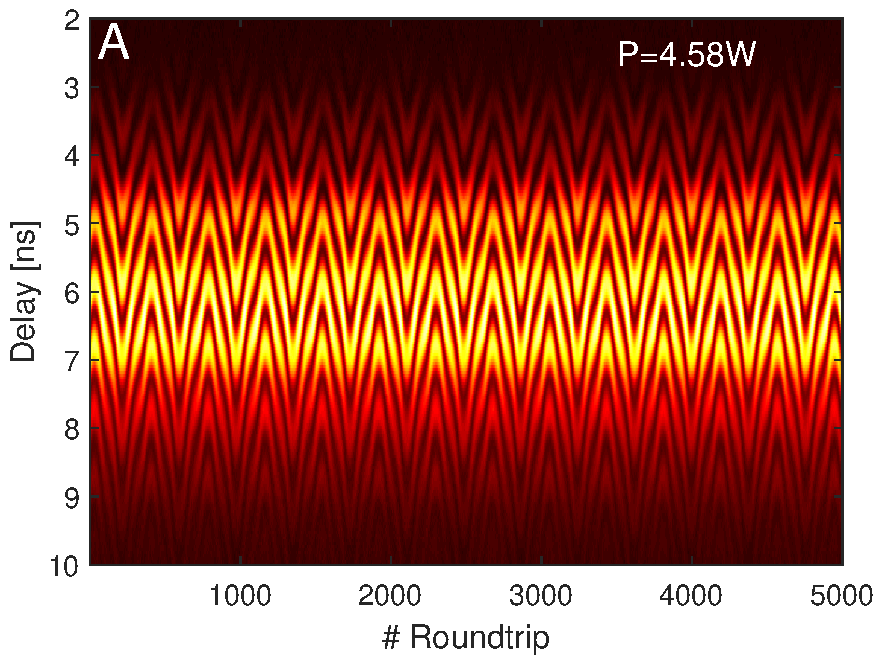
\includegraphics[width=0.49\textwidth]{figures/4ms_25GSA_400m_MLrun_runBounceFix_4,58W_Ch_PWnoCB}}
   \hfill
   \subfloat[\label{fig:rBF463}]
   {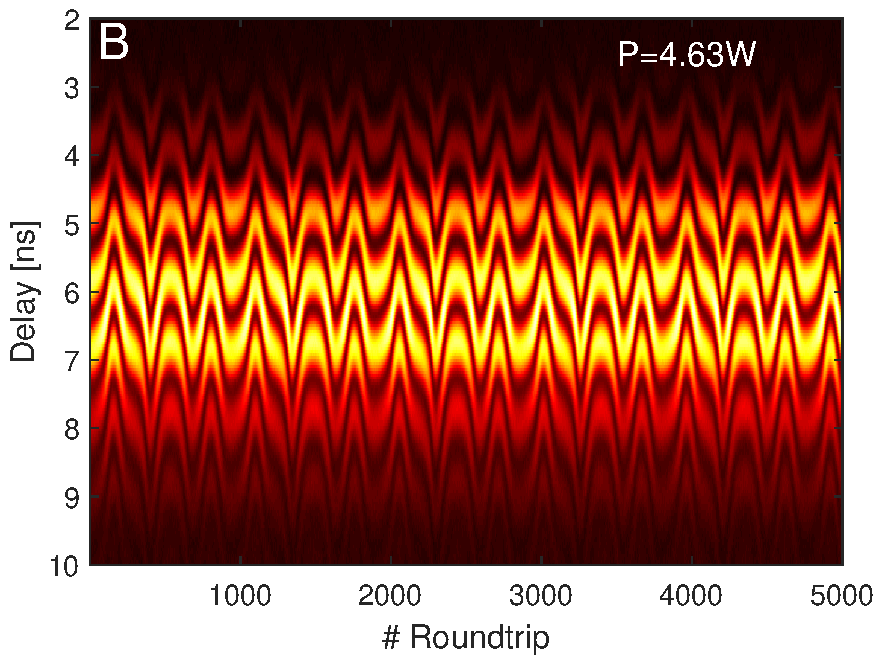
\includegraphics[width=0.49\textwidth]{figures/4ms_25GSA_400m_MLrun_runBounceFix_4,63W_Ch_PWnoCB}}
   
   \subfloat[\label{fig:rBF464}]
   {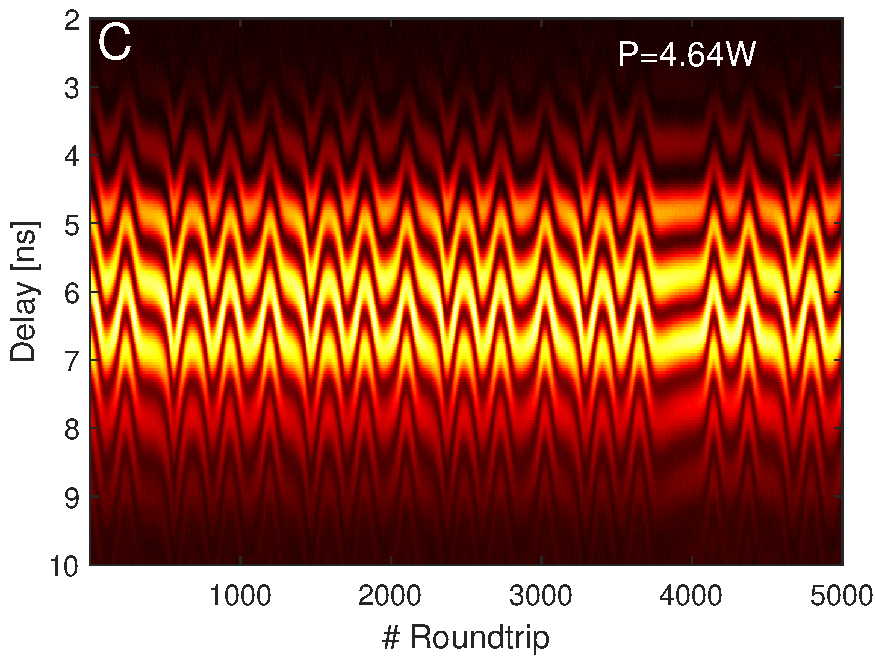
\includegraphics[width=0.49\textwidth]{figures/4ms_25GSA_400m_MLrun_runBounceFix_4,64W_Ch_PWnoCB}}
   \hfill
   \subfloat[\label{fig:rBF468}]
   {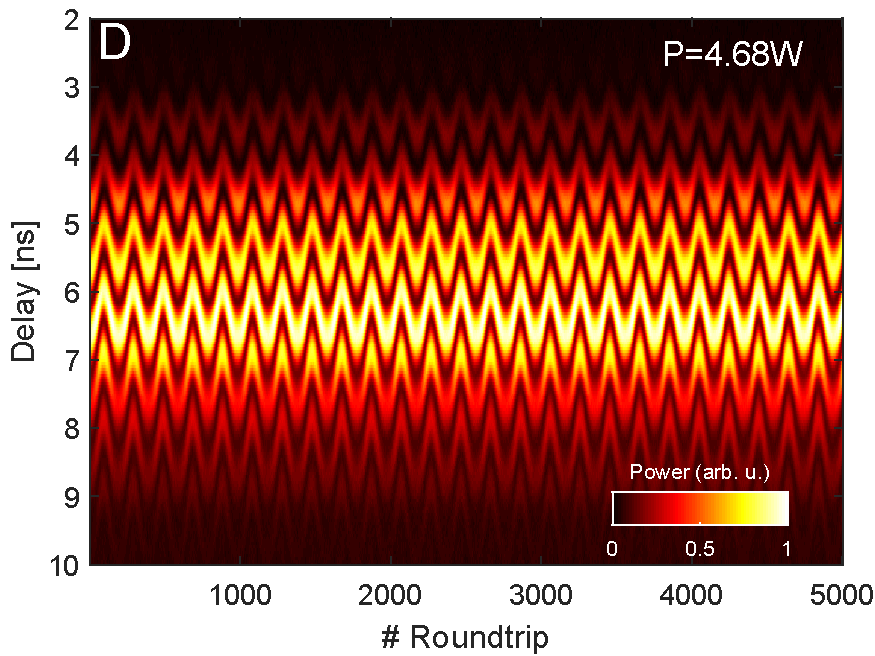
\includegraphics[width=0.49\textwidth]{figures/4ms_25GSA_400m_MLrun_runBounceFix_4,68W_Ch_PWwithCB}}
   \caption{Gebundene Pulse: Zeitaufgelöste Spektren bei Änderung der Pumpleistung.}
   \label{fig:boundSpectro}
\end{figure}
 
Für drei der in Abbildung \ref{fig:boundSpectro} gezeigten Messreihen wird das Verhalten exemplarisch diskutiert und die Dynamik in die \textit{Interaction Plane} eingezeichnet, also als polarer Plot mit dem Abstand als Radius und der Phase als Winkel.
In Abbildung \ref{fig:interactionPlane} ist jedoch der Radius um 80\,fs verringert, damit Abstandsänderungen besser zu erkennen sind.
Die Pfeile zeigen an, in welche Richtung die Orbits durchlaufen werden.
Für vergleichsweise niedrige sowie hohe Pumpleistungen ergibt sich ein Kreis-/Halbkreis-ähnliches Verhalten.
Im ersten Fall nimmt die relative Phase um etwa $2\pi$ zu, bevor diese sich diese Entwicklung umkehrt und die Phase um genau diesen Wert abnimmt bis es zur nächsten Umkehr kommt.
Gleichzeitig ändert sich der Abstand.
Für den Fall höherer Pumpleistung ist dies ähnlich: die Phase kehrt aber bereits nach einer Änderung um $\pi$ um.
Bei beiden Dynamiken fällt auf, dass der Abstand bei einer positiven Änderung der Phase zunimmt, während er bei einer Abnahme abnimmt.
Die der Pulsdynamik zugrunde liegende Gleichung \eqref{eq:ginzburgLandau} lässt darauf schließen, dass die Entwicklung der relativen Phase anzeigt, welcher Puls der stärkere ist.
Je intensiver ein Puls ist, desto mehr Selbstphasenmodulation erfährt er.
Somit wächst die absolute Phase schneller an.
Ist der erste Puls stärker, sollte also die relative Phase abnehmen.
Mit diesem Wissen lässt sich nun das oszillatorische Verhalten erklären:
Der vordere Puls ist der intensivere, die Phase nimmt ab, aber auch der Abstand, da der hintere Puls schwächer und somit schneller ist als der vordere.
Dieses Verhalten kehrt sich bei einem bestimmten Mindestabstand um.
Nun ist der vordere der schwächere, die Phase und der Abstand nehmen zu, bis ein bestimmter Maximalabstand erreicht wird.
Danach beginnt der Prozess erneut.

Dieser Zusammenhang zwischen der Änderung der Phase und des Abstandes ist auch für das komplexere Verhalten bei mittlerer Pumpleistung zu beobachten.
Dort ergibt sich auch ein geschlossener Orbit.
Dieser folgt teilweise den beiden anderen Dynamiken, besitzt jedoch 6 Umkehrpunkte.
Außerdem nimmt die Phase langfristig ab, der hintere Puls ist also durchschnittlich schwächer als der vordere.
 \begin{figure}[!htb]
	\centering
	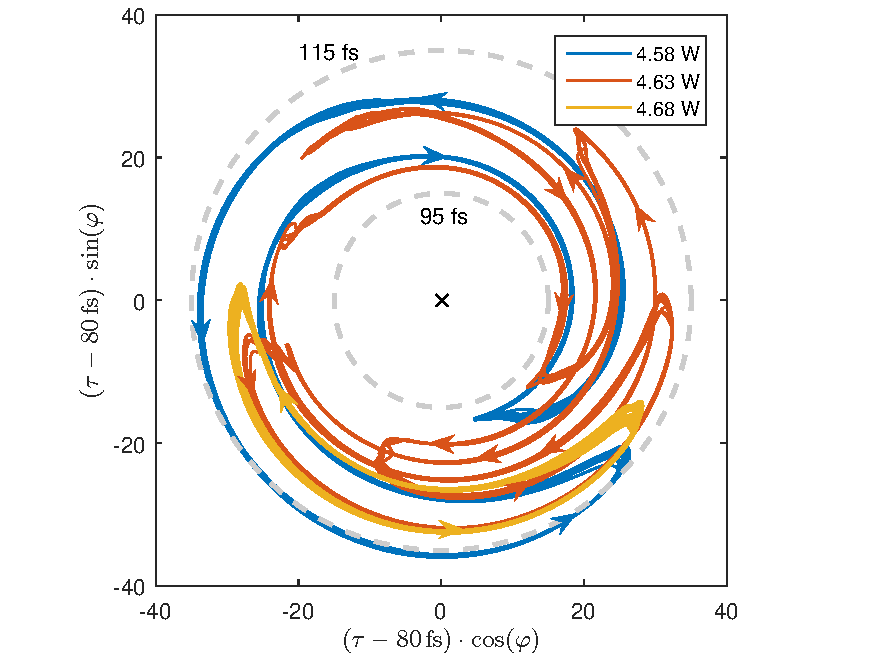
\includegraphics[width=0.73\textwidth]{figures/4ms_25GSA_400m_MLrun_runBounceFix_InteractionPlaneArrows_final2.pdf}
	\caption{Gebundene Pulse: Phasendynamik in der Interaction Plane  in Abhängigkeit der Pumpleistung.
	Während sich bei niedriger (blau) und hoher Pumpleistung (gelb) ein Kreis/Halbkreis-ähnliches Verhalten zeigt, ist die Dynamik bei einer mittleren Pumpleistung (rot) deutlich komplexer. Trotzdem ergibt sich ein geschlossener Orbit.}
	\label{fig:interactionPlane}
\end{figure}
\clearpage
\subsection{Kollidierende Pulse (mittlere Pumpleistung)}
\label{sec:bounce}
Dieser Zustand ist dadurch gekennzeichnet, dass es ständig zu Kollisionen zwischen den beiden Pulsen kommt, wie in Abbildung \ref{fig:rBF456} gut zu erkennen ist.
Diese entfernen sich danach schnell voneinander bevor der Abstand beider Pulse linear abnimmt und es schließlich zur erneuten Kollision kommt.
Erklären lässt sich dies damit, dass sich nach der Kollision ein schwacher Puls vor dem starken ausbildet, dieser aufgrund des Kerr-Effektes schneller durch den Resonator läuft und somit der Abstand beider größer wird.
Dann kommt es jedoch zu einem Anwachsen des vorderen Pulses und zu einer Schwächung des hinteren, weil dieser nur die vom Vorderen reduzierte Besetzungsinversion sieht und so weniger Verstärkung erfährt.
Es stellt sich ein festes Intensitätsverhältnis und somit auch eine konstante Relativgeschwindigkeit ein, mit der sich beide annähern, bis es zur nächsten Kollision kommt (vgl. Abb. \ref{fig:bounceZyklus}, in welcher ein solcher Zyklus zu sehen ist).
Somit lässt sich auch erklären, warum die Kollisionszeit $T_\text{interColl.}$, also die Zeit zwischen zwei Kollisionen, linear mit der maximalen Entfernung $\tau_\text{max}$ zusammenhängt (Abb. \ref{fig:bounceDistTime}).
Die Pulse entfernen sich meist mehr als 700\,fs und benötigen meist mehr als 3000 Roundtrips, also etwa $40\,\si{\micro\second}$, zwischen zwei aufeinanderfolgenden Kollisionen.
Diese Werte sind auch von der Pumpleistung abhängig.
Da sich die Pulse bei geringen Pumpleistungen aber teilweise auch weiter als 1\,ps voneinander entfernen, kann in diesen Fällen der maximale Abstand nicht mehr aufgelöst werden.
Interessant wäre jedoch, ob sich auch bei anderen Pumpleistungen Häufungen des maximalen Abstandes wie in Abbildung \ref{fig:rBF456histo} bei $P_\text{Pump}=4.56\,$W ergeben.

\begin{figure}[!htb]
   \centering   
   \subfloat[Ausschnitt der Autokorrelation\label{fig:rBF456}]
   {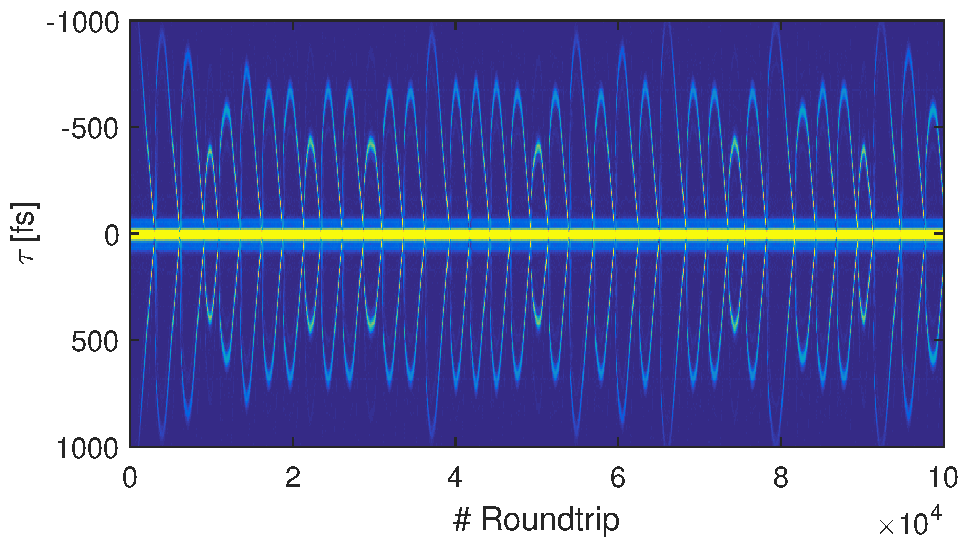
\includegraphics[width=0.58\textwidth]{figures/4ms_25GSA_400m_MLrun_runBounceFix_4,56W_Ch1_150000_250000_autocorr_stretch}}
   \hfill
   \subfloat[Histogramm des maximalen Pulsabstandes $\tau_\text{max}$ vor jeder Kolllision\label{fig:rBF456histo}]
   {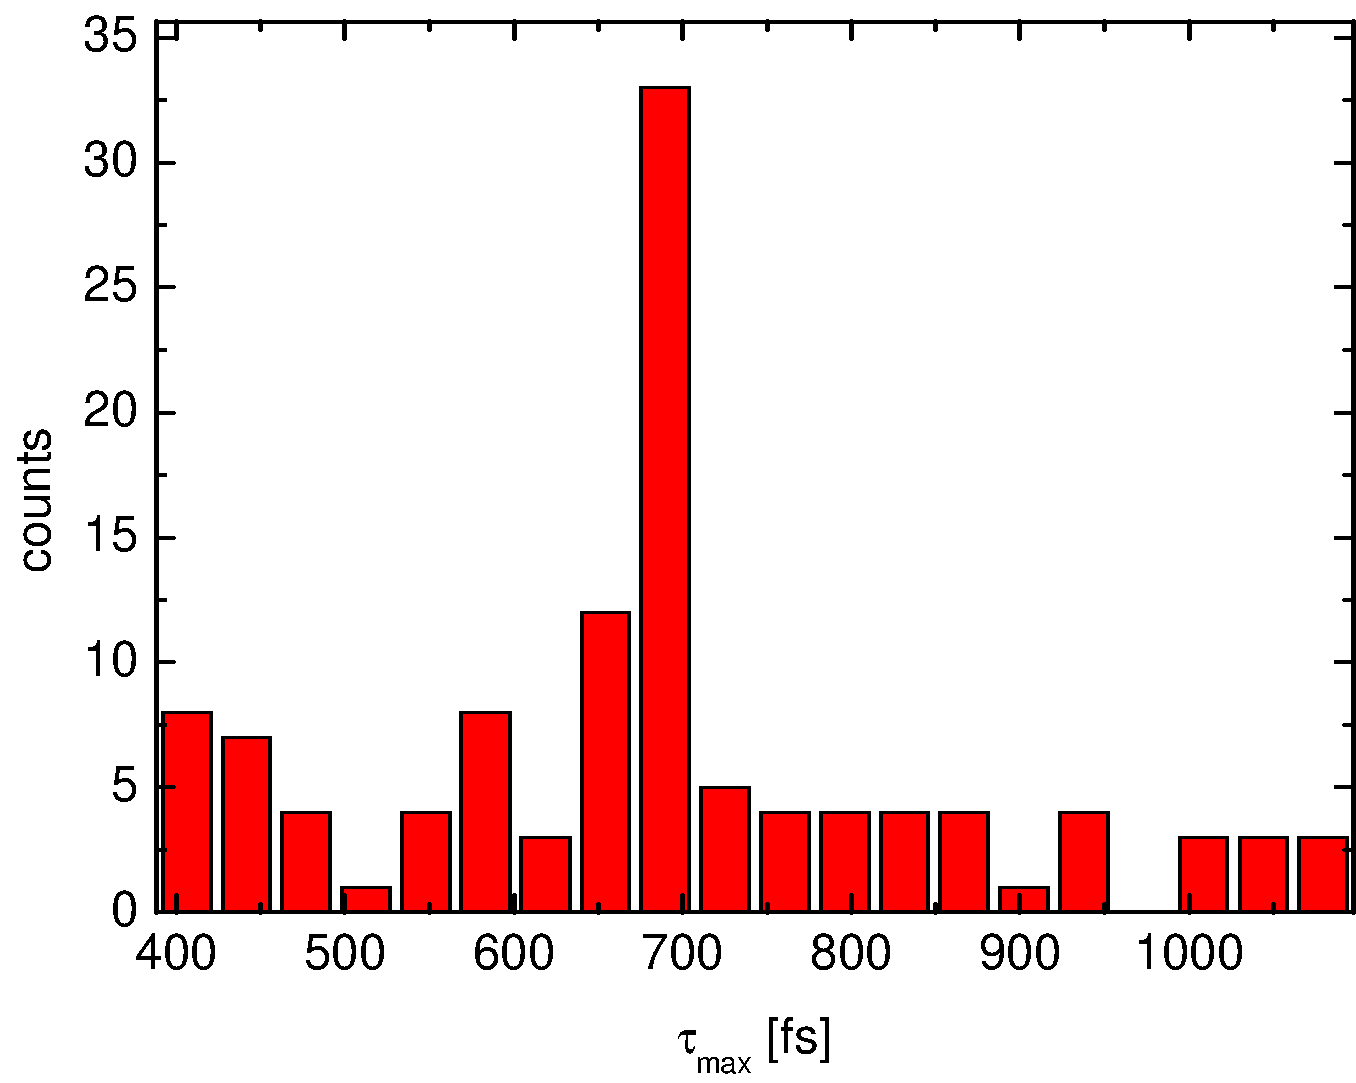
\includegraphics[width=0.4\textwidth]{figures/bounce456histo}}
   \caption{Kollidierende Pulse bei einer Pumpleistung von $4.56\,$W.}
   \label{fig:bouncing456}
 \end{figure}

\begin{figure}[!htb]
   \centering 
   \subfloat[spektrale Ansicht\label{fig:bounceZyklusSpectrum}]
   {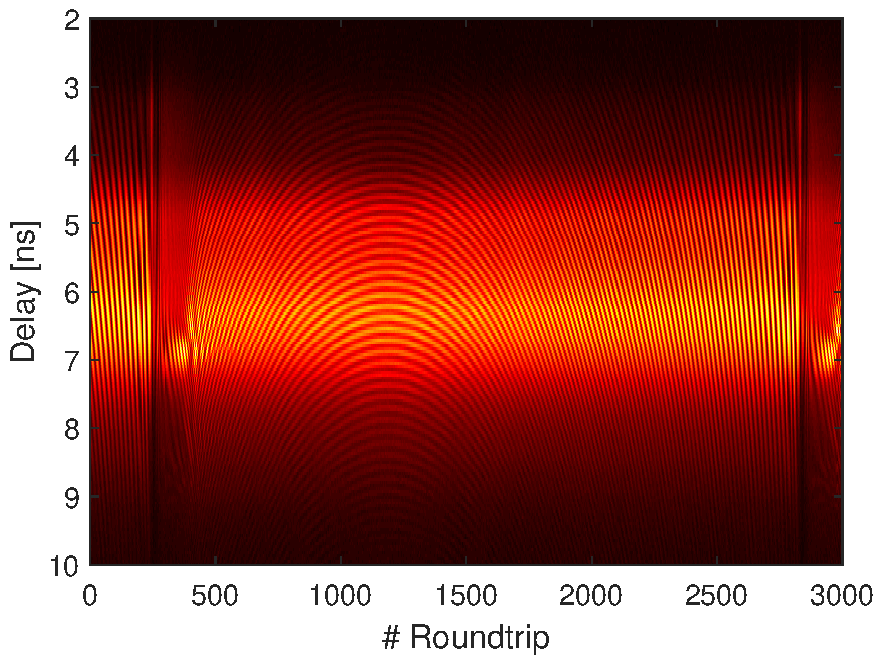
\includegraphics[width=0.49\textwidth]{figures/4ms_25GSA_400m_MLrun_runBounceFix_4,56W_Ch1_141000_144000_spectrum}}
   \hfill
   \subfloat[Autokorrelation \label{fig:bounceZyklusAutocorr}]
   {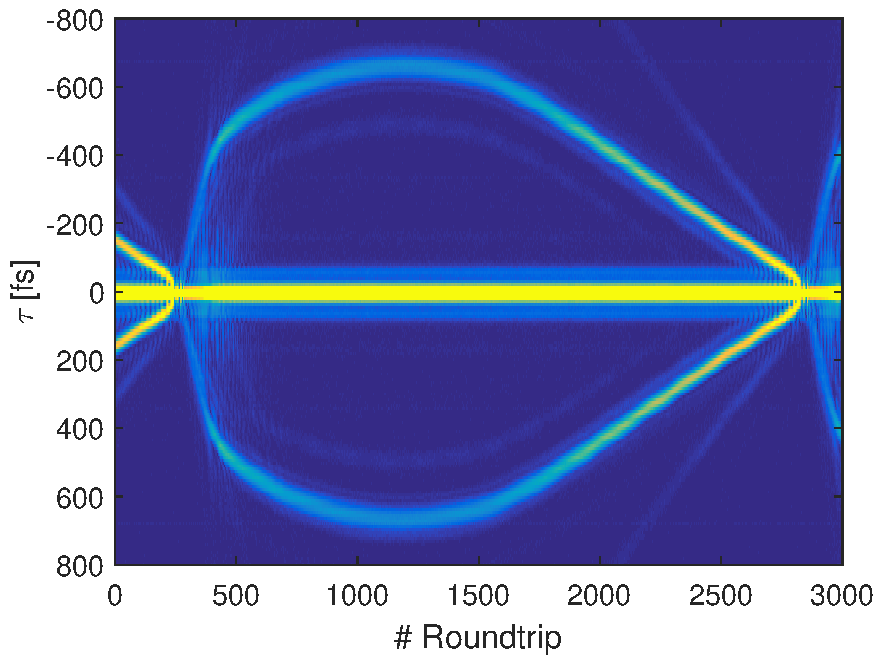
\includegraphics[width=0.49\textwidth]{figures/4ms_25GSA_400m_MLrun_runBounceFix_4,56W_Ch1_141000_144000_autocorr}}
   \caption{Kollisionszyklus ($P_\text{Pump}=4.56\,$W)}
   \label{fig:bounceZyklus}
\end{figure}
 
\begin{figure}[!htb]
	\centering
	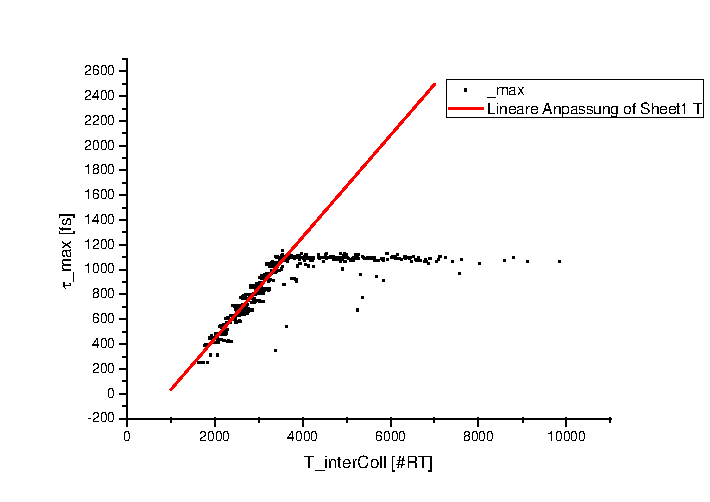
\includegraphics[width=0.55\textwidth]{figures/bounceDistTime}
	\caption{Maximaler Pulsabstand $\tau_\text{max}$ versus Zeit zwischen zwischen zwei Kollisionen $T_\text{interColl.}$. Das bestimmte $\tau_\text{max}$ ist begrenzt durch die maximale Modulationsfrequenz des Spektrums.}
	\label{fig:bounceDistTime}
\end{figure}

Wenn die Pumpleistung auf 4.57\,W erhöht wird, zeigt sich noch ein weiterer Interaktionsmechanismus: Die beiden Pulse stoßen sich voneinander ab, bevor sie überhaupt kollidieren.
Diese Pumpleistung ist genau am Übergangsbereich zu den im vorigen Abschnitt beschriebenen gebundenen Doppelpulsen.
In Abbildung \ref{fig:rBF457} ist der Unterschied zu erkennen: Im Kollisionsfall entfernen sich die beiden Pulse wesentlich schneller und weiter.
Außerdem ist eine klare Asymmetrie bezüglich des Kollisionszeitpunktes zu erkennen, während beim Abstoßungsprozess Annähern und Entfernen fast gleich ablaufen.
In beiden Fällen ist beim Annähern eine Interaktion bzgl. der relativen Phase zu beobachten.


\begin{figure}[!htb]
   \centering
   \captionsetup[subfloat]{farskip=18pt}
   \subfloat[Überblick.\label{fig:rBF457_autocorr}]
   {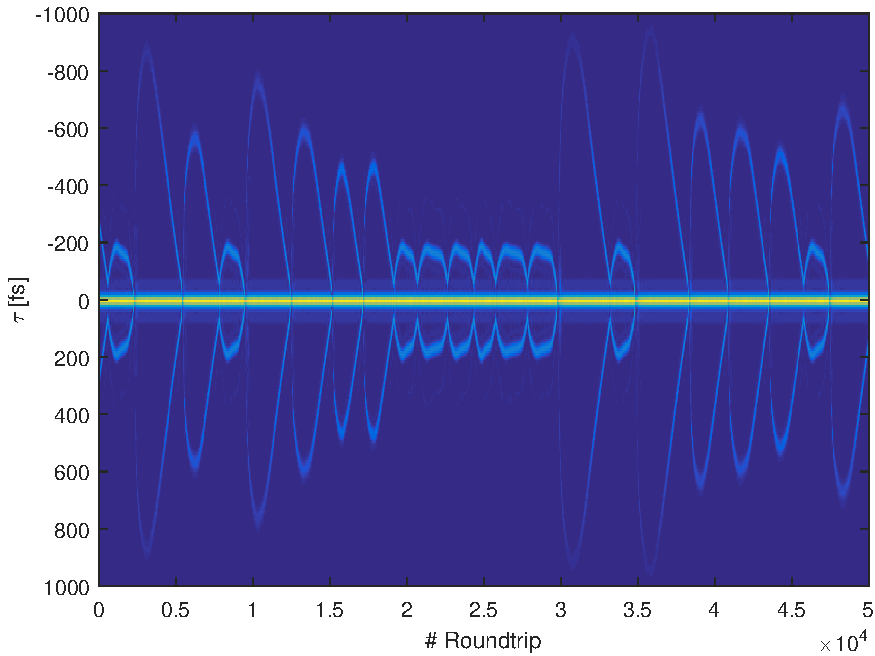
\includegraphics[width=0.49\textwidth]{figures/4ms_25GSA_400m_MLrun_runBounceFix_4,57W_Ch1_120000_170000_autocorr}}
   \hfill
   \subfloat[Zoom.\label{fig:rBF457_autocorr_zoom}]
   {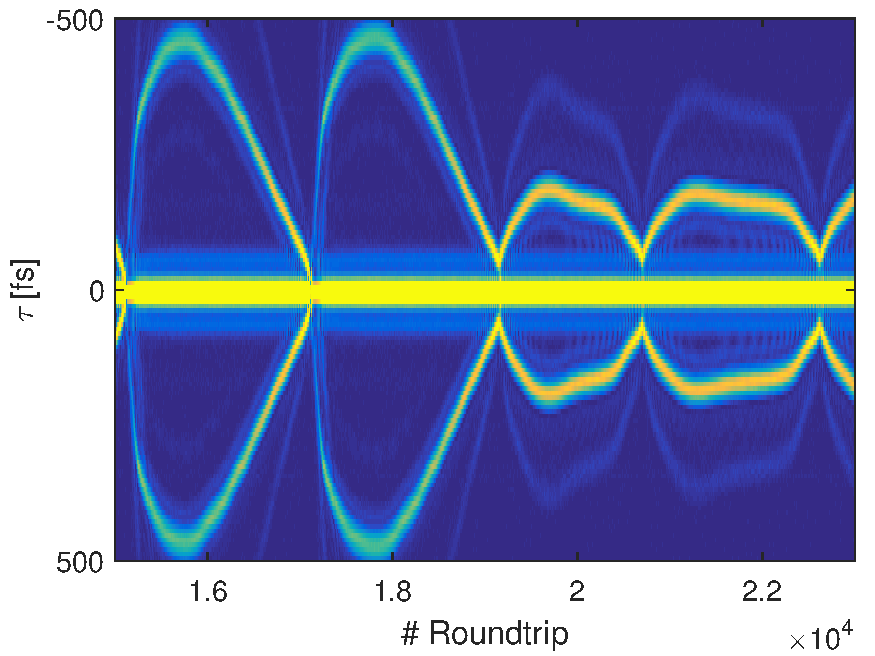
\includegraphics[width=0.49\textwidth]{figures/4ms_25GSA_400m_MLrun_runBounceFix_4,57W_Ch1_135000_143000_autocorr}}
   
   \subfloat[Kollision, spektrale Ansicht.\label{fig:rBF457_coll_spec}]
   {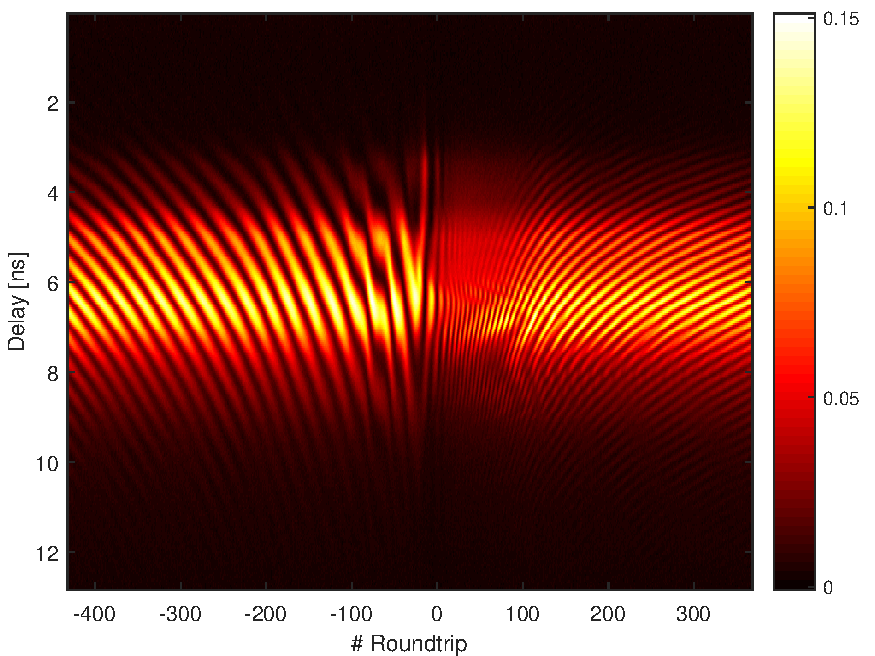
\includegraphics[width=0.49\textwidth]{figures/4ms_25GSA_400m_MLrun_runBounceFix_4,57W_Ch1_136700_137500_spectrum}}
   \hfill
   \subfloat[Kollision, Autokorellation.\label{fig:rBF457_coll_autocorr}]
   {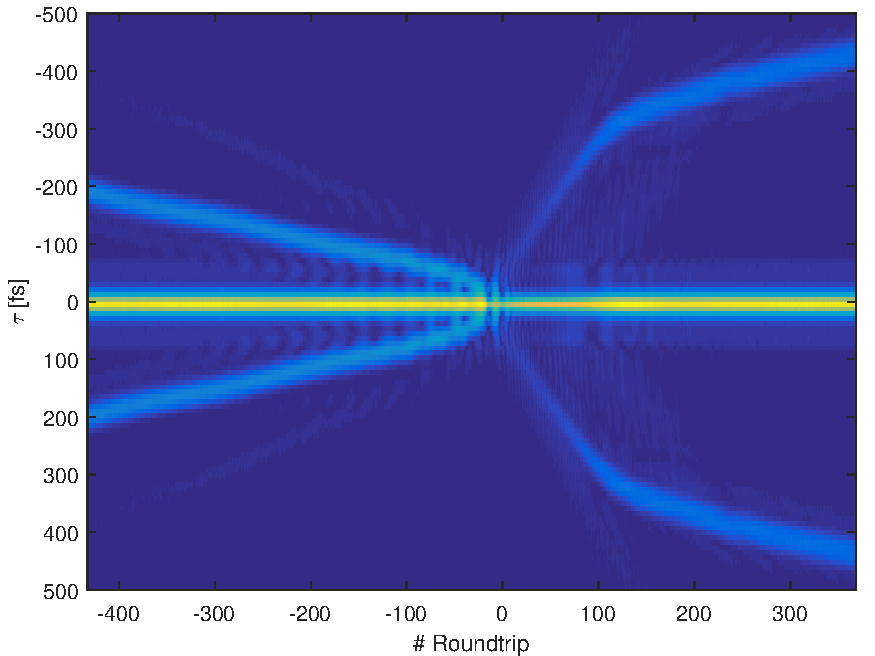
\includegraphics[width=0.49\textwidth]{figures/4ms_25GSA_400m_MLrun_runBounceFix_4,57W_Ch1_136700_137500_autocorr}}
   
   \subfloat[Abstoßung, spektrale Ansicht.\label{fig:rBF457_repel_spec}]
   {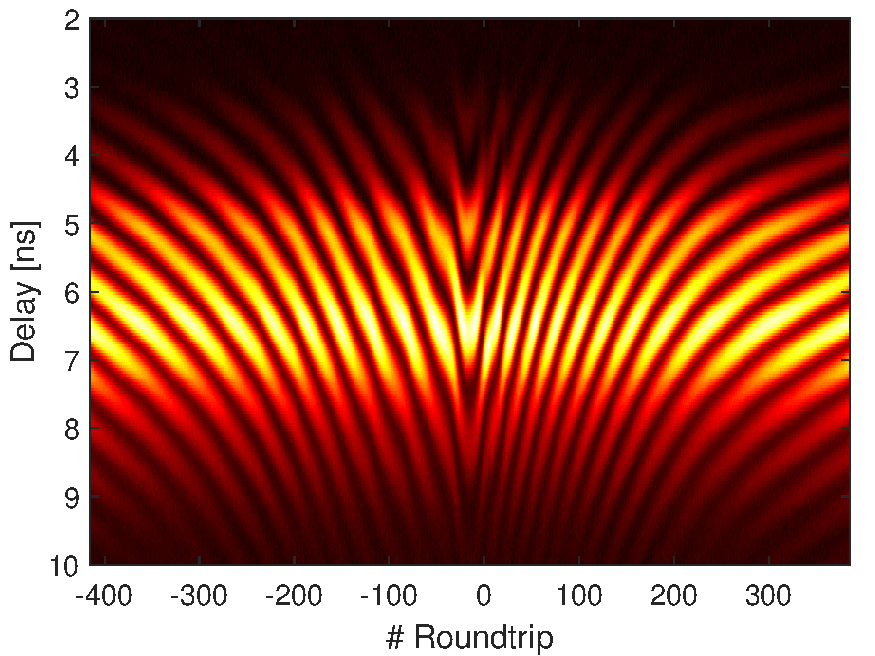
\includegraphics[width=0.49\textwidth]{figures/4ms_25GSA_400m_MLrun_runBounceFix_4,57W_Ch1_140300_141100_spectrum}}
   \hfill
   \subfloat[Abstoßung, Autokorrelation.\label{fig:rBF457_repel_autocorr}]
   {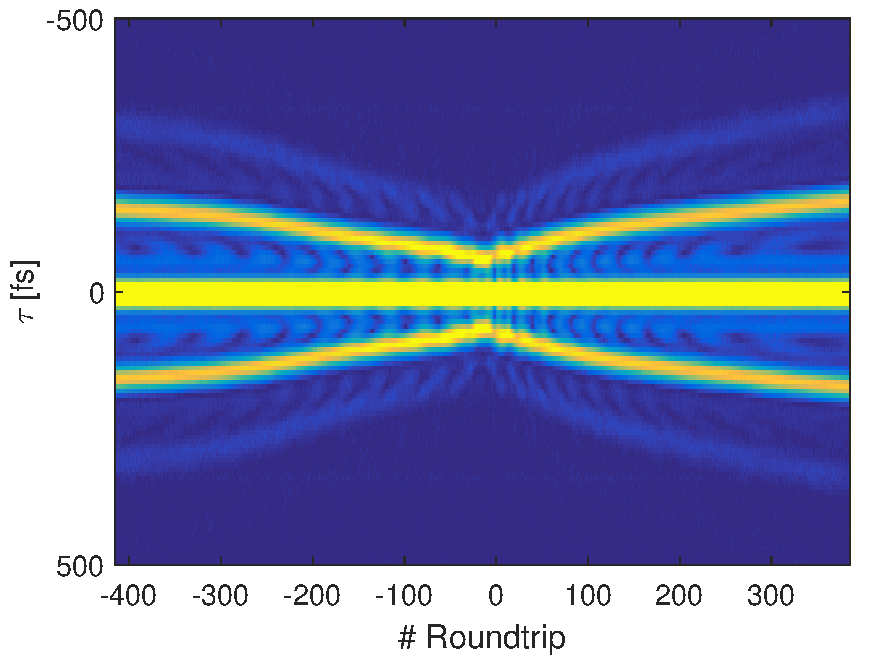
\includegraphics[width=0.49\textwidth]{figures/4ms_25GSA_400m_MLrun_runBounceFix_4,57W_Ch1_140300_141100_autocorr}}
   \caption{$P_\text{Pump}=4.57\,$W: Unterschied zwischen Kollision und Abstoßung der beiden Pulse.}
   \label{fig:rBF457}
\end{figure}

\subsection{Durchlaufende Pulse (niedrige Pumpleistung)}
In diesem Zustand ist die Pumpleistung so gering, dass zwar zwei Pulse durch den Laser laufen, diese aber einen großen Intensitätsunterschied haben, so dass sie unterschiedliche optische Weglängen haben und sich so auf einer 100\,ms-Skala gegeneinander verschieben.
In Abb. \ref{fig:rBF441} ist eine \textit{FastFrame}-Aufnahme dieses Betriebs zu sehen.
Dabei wird auf den stärkeren Puls getriggert.
Es wird im Gegensatz zu den anderen Aufnahmen nicht kontinuierlich gemessen, indem zu jedem Roundtrip das Spektrum und zeitliches Signal aufgenommen wird.
Hier werden sehr viele Pulse übersprungen, damit ein langes Zeitintervall von $400\,\si{\milli\second}$ auch mit 25\,GSa/s  aufgenommen werden kann.
Bei der abgebildeten Messreihe vergehen $5\,\si{\micro\second}$ zwischen je zwei Triggerzeitpunkten.
Die Relativgeschwindigkeit zwischen beiden Pulsen ist jedoch nur annähernd konstant.
Dies lässt sich auch in der Peak-Spannung des undispergierten Signals erkennen, welche proportional zur Pulsenergie ist (vgl. Abb. \ref{fig:rBF441peakTau}).
So wird der schwache Puls die meiste Zeit schwächer, während der starke stärker wird.
Dies führt zu einer Zunahme der Relativgeschwindigkeit.
Es gibt jedoch zwei Zeitpunkte zwischen zwei aufeinanderfolgenden Kollisionen, bei denen sich dieses Verhalten genau umgekehrt: Es findet ein Energietransfer vom stärkeren zum schwächeren Puls statt und die Relativgeschwindigkeit nimmt ab.
Dies lässt sich damit erklären, dass die beiden Pulse sich gerade dann im Laserkristall begegnen und so der schwächere Puls vom Kerr-Effekt durch den stärkeren profitiert.

\begin{figure}[!htb]
   \centering   
   \subfloat[\textit{FastFrame}-Aufnahme des Zeitsignals\label{fig:rBF441}]
   {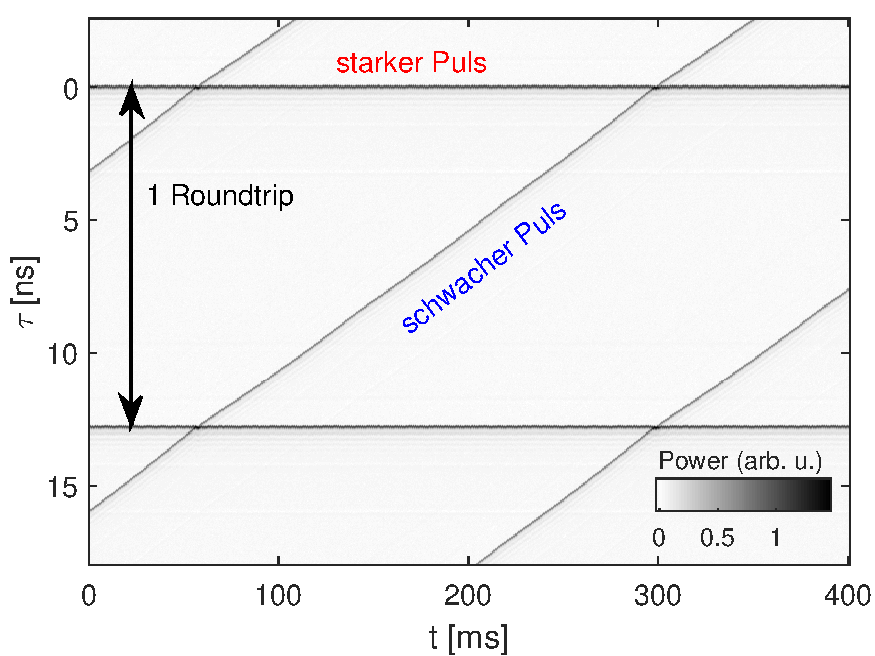
\includegraphics[width=0.51\textwidth]{figures/400ms_5musHold_25GSA_400m_MLrun_runBounceFix_4,41W_Ch2CB_arrows}}
   \hfill
   \subfloat[Zeitliche Entwicklung der beiden Puls\-energien und der Differenz der Umlaufzeit\label{fig:rBF441peakTau}]
   {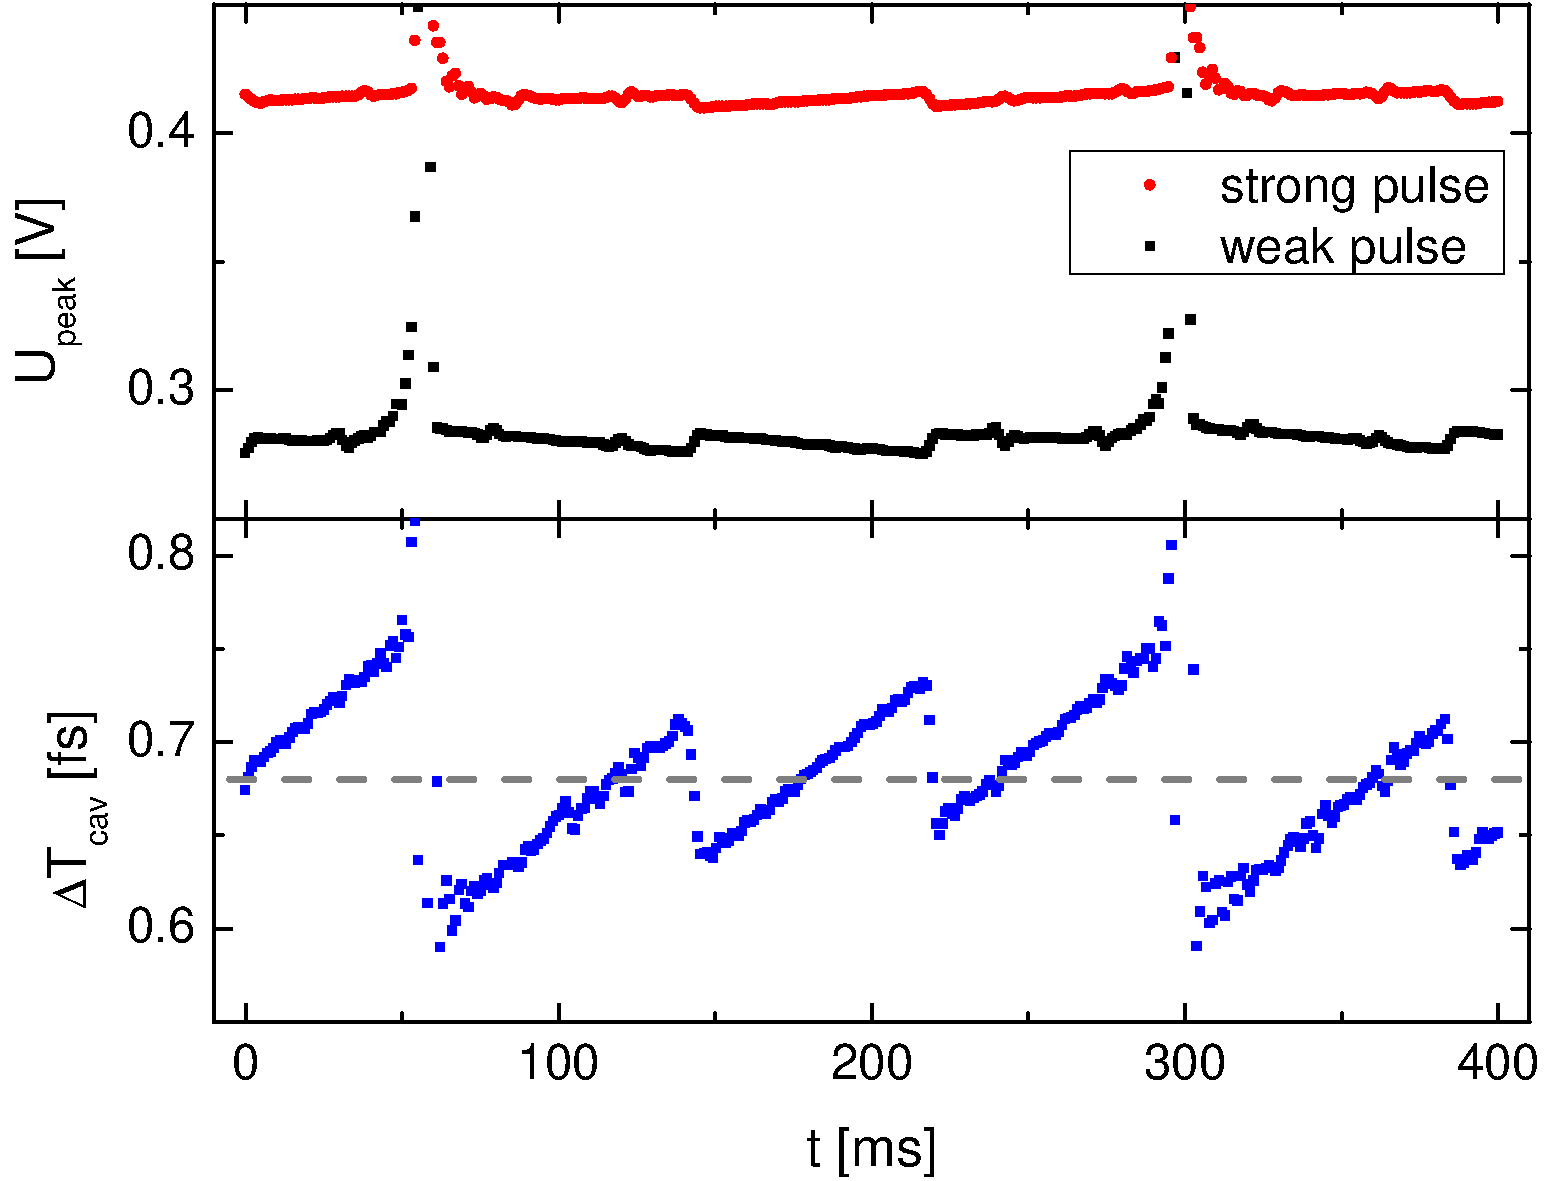
\includegraphics[width=0.48\textwidth]{figures/runningPeakTau}}
   \caption{Zwei unterschiedlich starke Pulse im Laser, die aufgrund des Kerr-Effekts verschiedene optische Weglängen vorfinden und sich so gegeneinander verschieben.}
   \label{fig:running441}
 \end{figure}


\section{Doppelpulse Messreihe 2}
Bei dieser Messreihe ist der Laser etwas besser justiert als zuvor, sodass die Ausgangsleistung höher ist und somit sogar Dreifachpulse möglich sind.
Durch Störung des Einzelpuls-Betriebs und anschließendes Variieren der Pumpleistung lassen sich wieder verschiedene Multipulsdynamiken finden.
Unter anderem wird bei einer deutlich geringeren Pumpleistung das in Abschnitt \ref{sec:oscillatingSolitons} beschriebene oszillatorische Verhalten der Phase und des Abstandes gebundener Doppelpulse bei einem Abstand von 100\,fs beobachtet.
In diesem Abschnitt wird jedoch das Verhalten von 170\,fs entfernten Doppelpulsen gezeigt.
Darüber hinaus stehen die Triplett-Zustände im Fokus.

\subsection{Stufenweise Phasenentwicklung gebundener Doppelpulse}
Hier beginnt die Messreihe mit Doppelpulsen, deren Phase und relativer Abstand fest sind (Abb. \ref{fig:165014steps} A+B).
Der Abstand liegt etwa bei 170 \,fs.
Dann wird die Pumpleistung verringert.
Dabei wird beobachtet, dass der Abstand der beiden Pulse immer noch sehr konstant ist, während die Phase jedoch beginnt, in $2\pi$-Sprüngen durchzulaufen (vgl. Abb. \ref{fig:165014steps} C-F).
Verringert sich die Pumpleistung weiter, geschieht dieser Prozess schneller, bis die Phase annähernd linear anwächst (vgl. Abb. \ref{fig:165014steps} G+H).
Je geringer die Pumpleistung ist, desto schneller wächst die relative Phase zwischen beiden Pulsen an.
Um dies zu verdeutlichen, ist in Abbildung \ref{fig:jumpRT} in Abhängigkeit der Pumpleistung die Anzahl der Roundtrips aufgetragen, innerhalb deren sich die Phase um $2\pi$ ändert.
Wird die Entwicklung der Phase wie in Abbildung \ref{fig:165014steps2} mit dieser Zeit skaliert, lässt sich der Übergang von einer nahezu stufenförmigen Entwicklung zum linearen Drift der Phase durch Verringerung der Pumpleistung noch besser beobachten.

Für dieses Verhalten lässt sich eine  mögliche Erklärung finden:
Ist die Pumpleistung gering, ist der Intensitätsunterschied zwischen beiden Pulsen konstant.
Der hintere erfährt weniger Verstärkung und ist deshalb schwächer.
Die Phase ändert sich linear.
Für hohe Pumleistungen hingegen kann es zu einem Locken der Phase kommen (siehe Abb. \ref{fig:165014steps} A,B).
Bei einer leicht geringeren Pumpleistung driftet die Phase langsam von der gelockten Position weg.
Ist der Unterschied zu groß, beschleunigt sich die Änderung der Phase bis diese sich wieder in der Nähe der gelockten Position befindet.
Der Intensitätsunterschied nimmt also kurzzeitig stark zu bis sich wieder ein annähernd stabiler Zustand eingestellt hat.
Je geringer die Pumpleistung, desto größer der Intensitätsunterschied und instabiler dieser Zustand.

\begin{figure}[!htb]
   \centering
   \captionsetup[subfigure]{labelformat=empty}
   \captionsetup[subfloat]{farskip=-10pt,captionskip=0pt}
   \subfloat[]{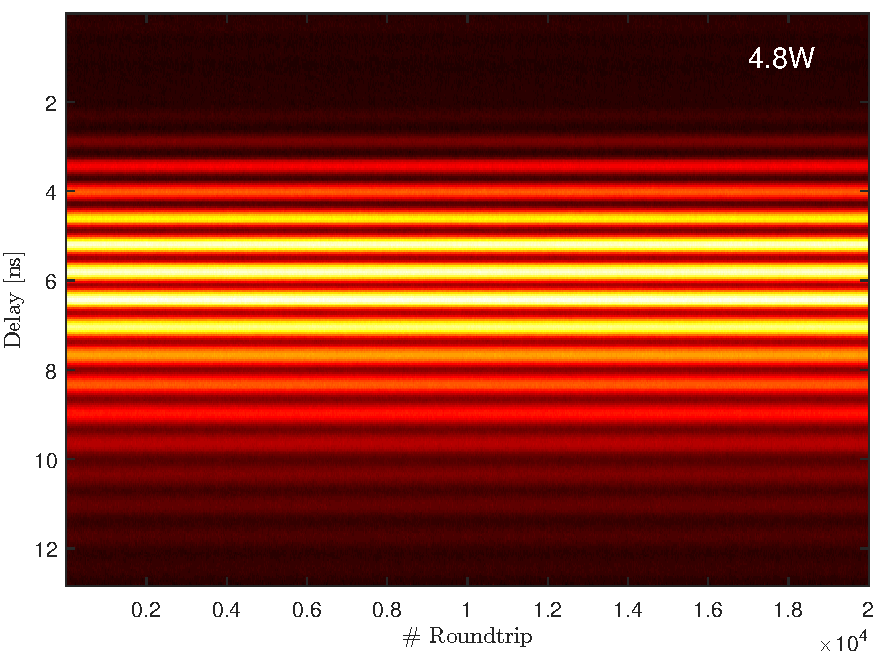
\includegraphics[width=0.49\textwidth]{figures/4ms_25GSA_400m_MLrun_Doppel4,8W_2_Ch_PWnoCB}}
   \hfill
   \subfloat[]
   {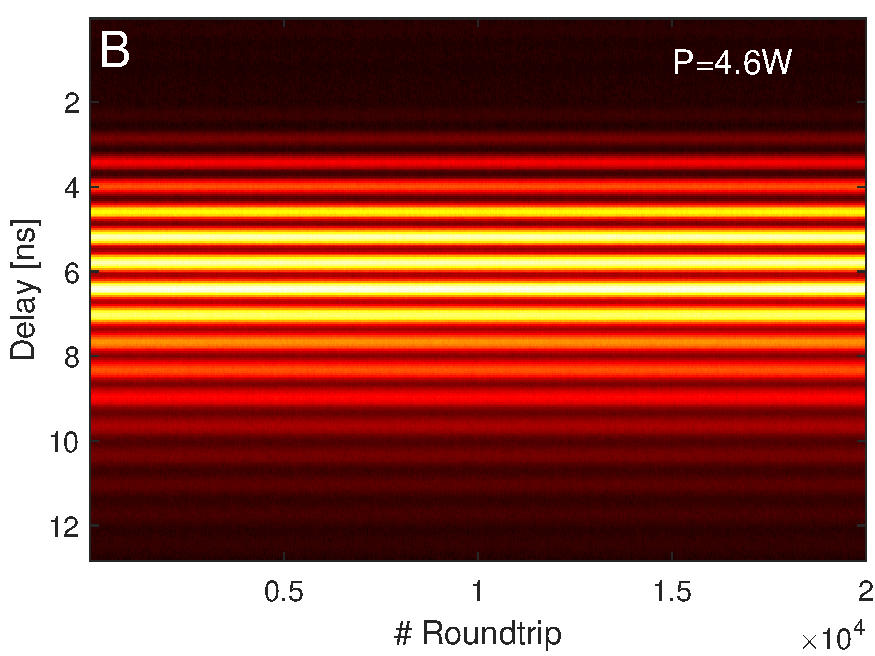
\includegraphics[width=0.49\textwidth]{figures/4ms_25GSA_400m_MLrun_Doppel4,6W_Ch_PWnoCB}}
   %\hfill
   
   \subfloat[]
   {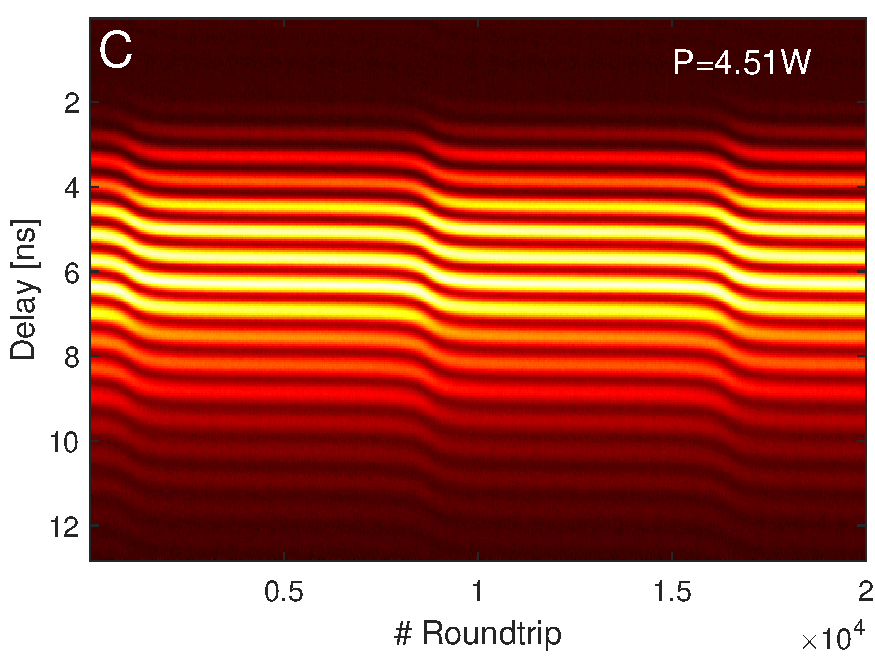
\includegraphics[width=0.49\textwidth]{figures/4ms_25GSA_400m_MLrun_Doppel4,51W_Ch_PWnoCB}}
   \hfill
   \subfloat[]
   {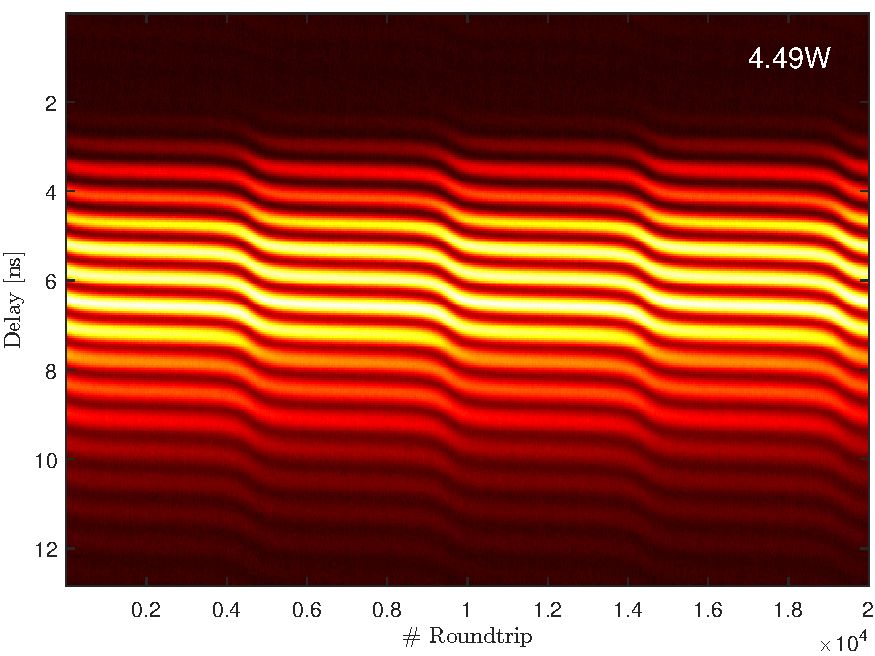
\includegraphics[width=0.49\textwidth]{figures/4ms_25GSA_400m_MLrun_Doppel4,49W_Ch_PWnoCB}}
   %\hfill
   
   \subfloat[]
   {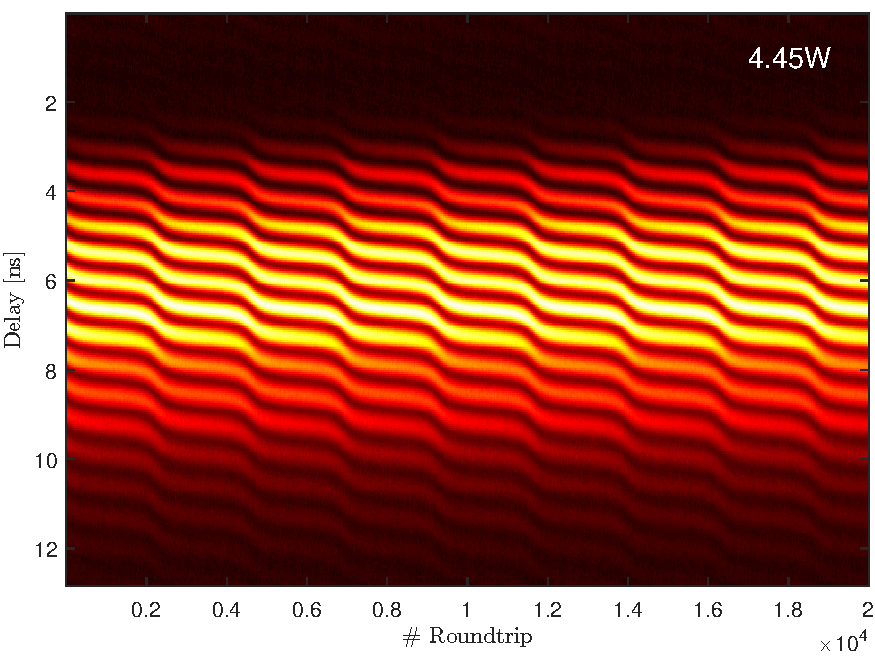
\includegraphics[width=0.49\textwidth]{figures/4ms_25GSA_400m_MLrun_Doppel4,45W_2_Ch_PWnoCB}}
   \hfill
   \subfloat[]
   {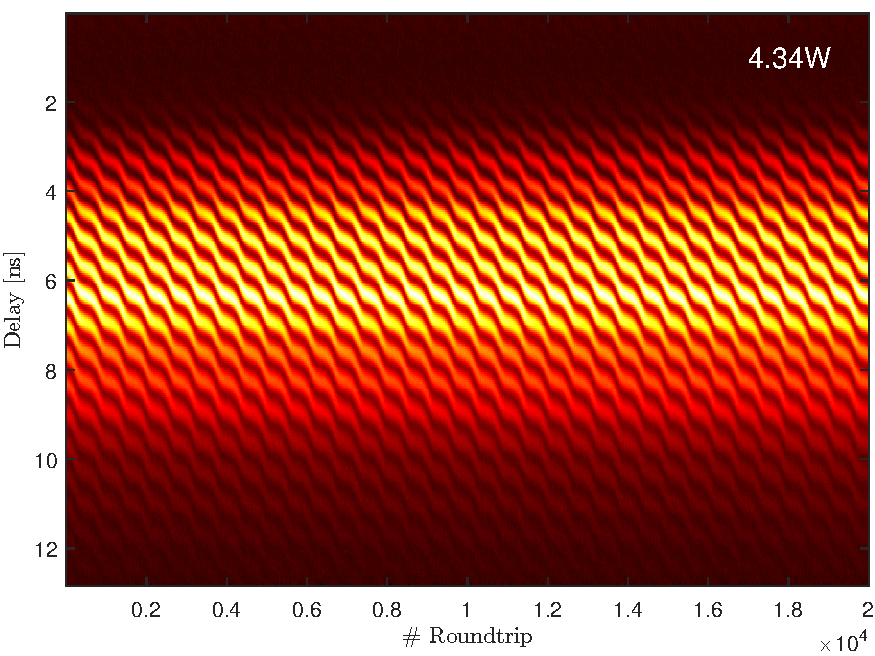
\includegraphics[width=0.49\textwidth]{figures/4ms_25GSA_400m_MLrun_Doppel4,34W_Ch_PWnoCB}}
   %\hfill
   
   \subfloat[]
   {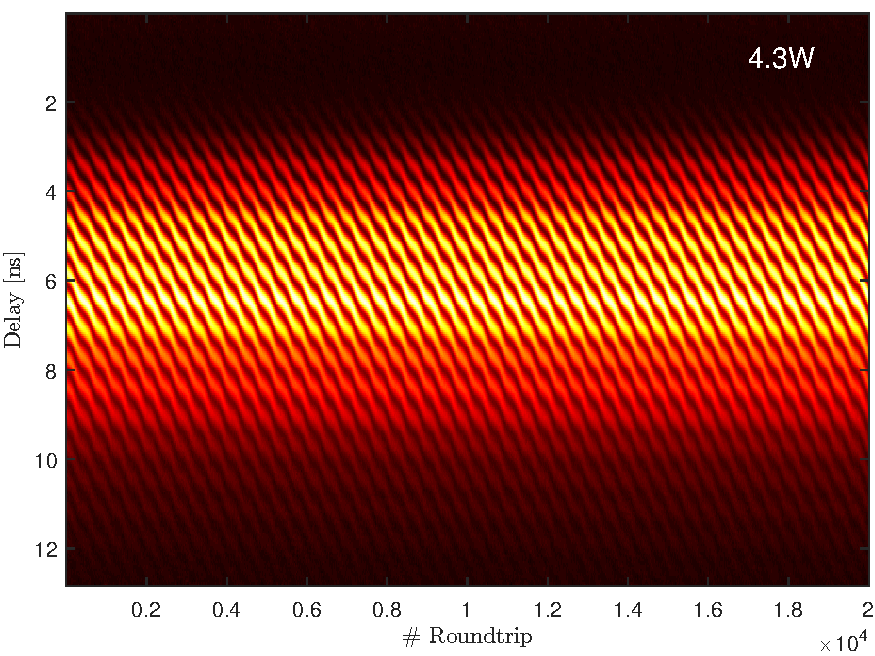
\includegraphics[width=0.49\textwidth]{figures/4ms_25GSA_400m_MLrun_Doppel4,3W_Ch_PWnoCB}}
   \hfill
   \subfloat[]
   {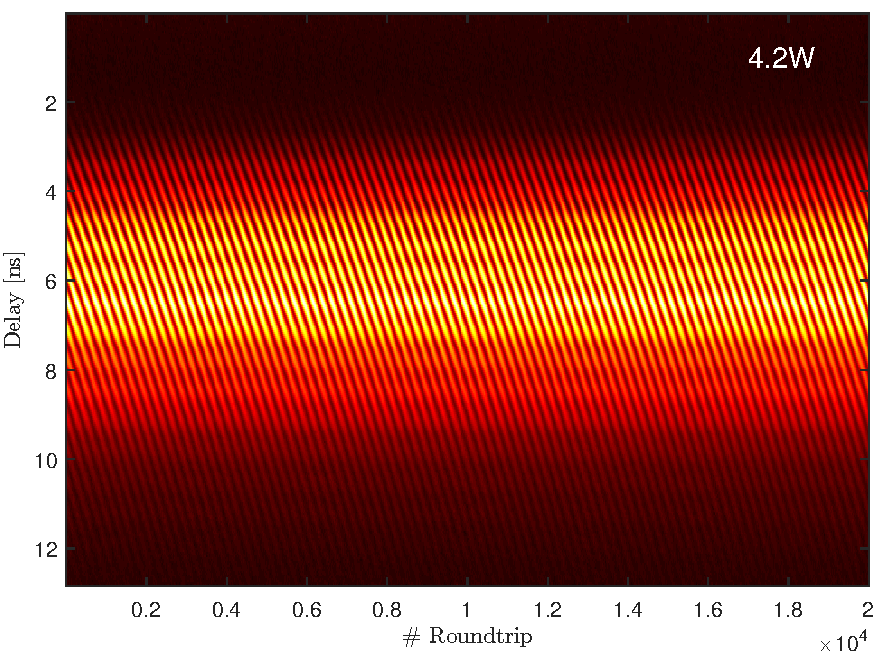
\includegraphics[width=0.49\textwidth]{figures/4ms_25GSA_400m_MLrun_Doppel4,2W_Ch_PWnoCB}}
   \caption{Verringerung der Pumpleistung: Von einer festen Phase über Stufen zu einer annähernd linear durchlaufenden Phase.}
   \label{fig:165014steps}
\end{figure}


\begin{figure}
	\centering
	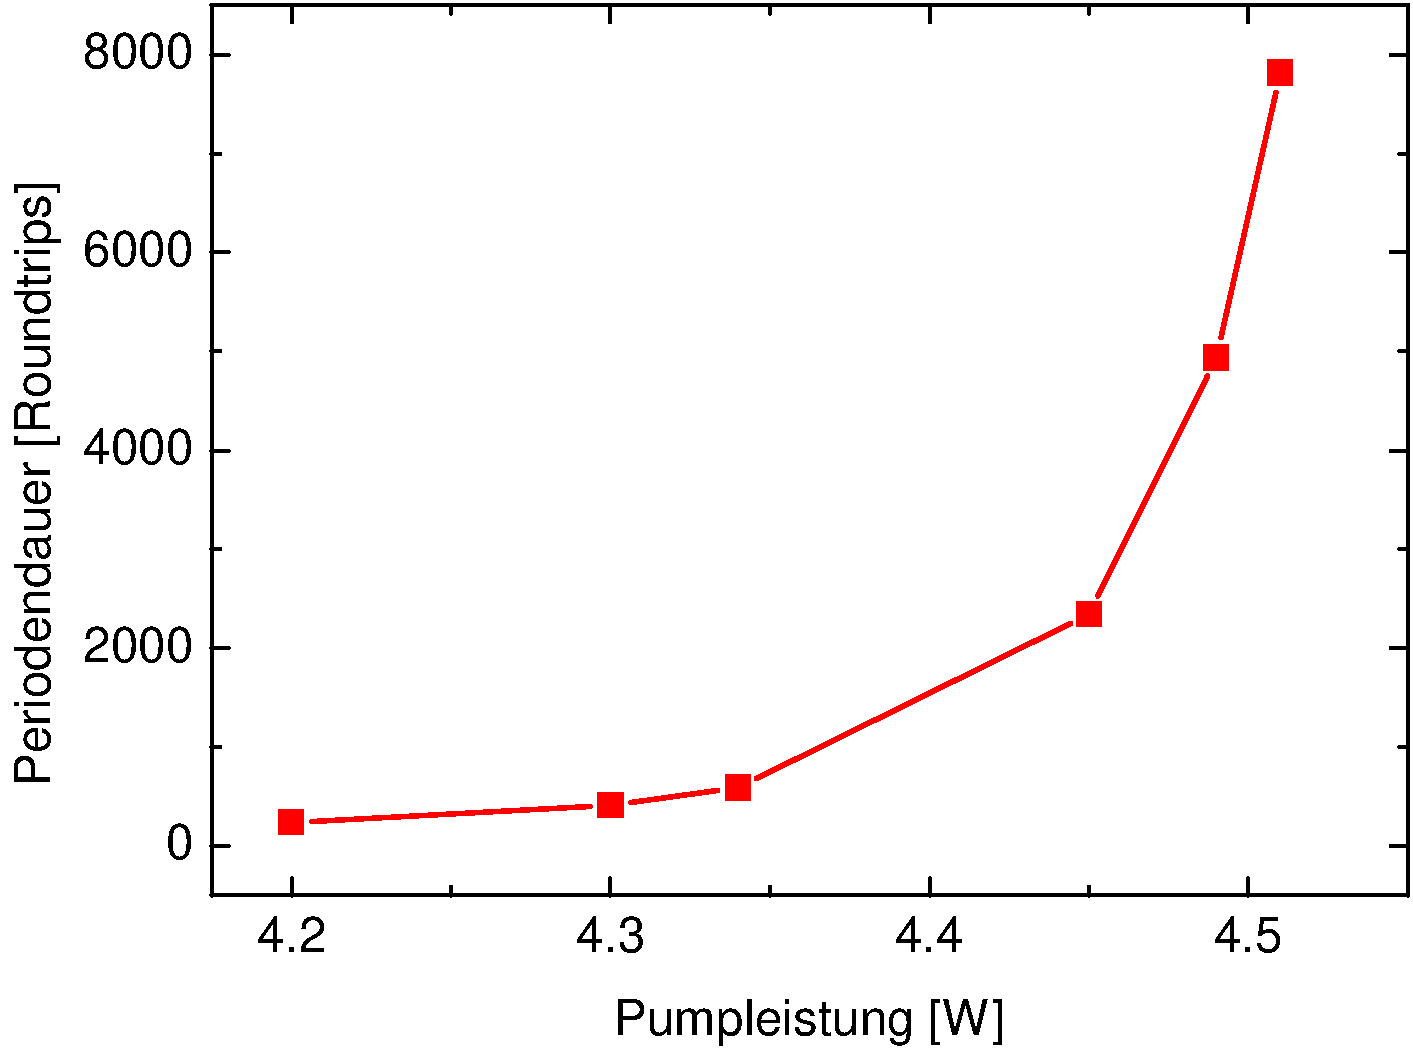
\includegraphics[width=0.7\textwidth]{figures/jumpRT.pdf}
	\caption{Anzahl an Roundtrips, innerhalb derer die relative Phase um $2\pi$ zunimmt, in Abängigkeit der Pumpleistung: Die relative Phase wächst bei niedrigen Pumpleistungen schneller an.}
   \label{fig:jumpRT}
\end{figure} 

\begin{figure}
	\centering
	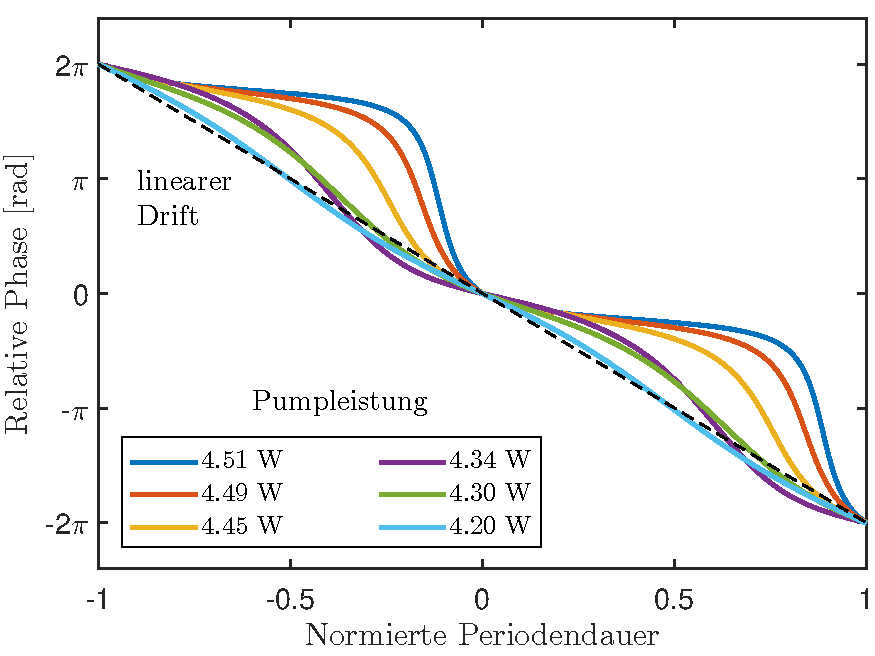
\includegraphics[width=0.7\textwidth]{figures/steps_relativ4.pdf}
	\caption{Phasenentwicklung über 2 Perioden für verschiedene Pumpleistungen mit der in Abb. \ref{fig:jumpRT} berechneten Zeit skaliert.}
   \label{fig:165014steps2}
\end{figure}


%\begin{figure}[!htb]
%   \centering
%   \captionsetup[subfigure]{labelformat=empty}
%   \captionsetup[subfloat]{farskip=-10pt,captionskip=0pt}   
%   \subfloat[]
%   {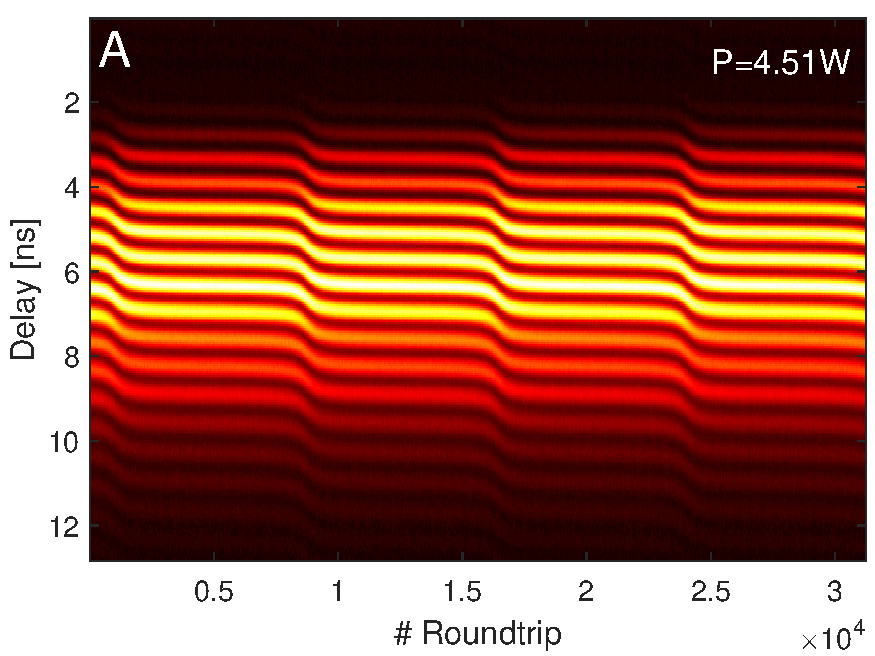
\includegraphics[width=0.49\textwidth]{figures/4ms_25GSA_400m_MLrun_Doppel4,51W_Ch_PWnoCB_scale}}
%   \hfill
%   \subfloat[]
%   {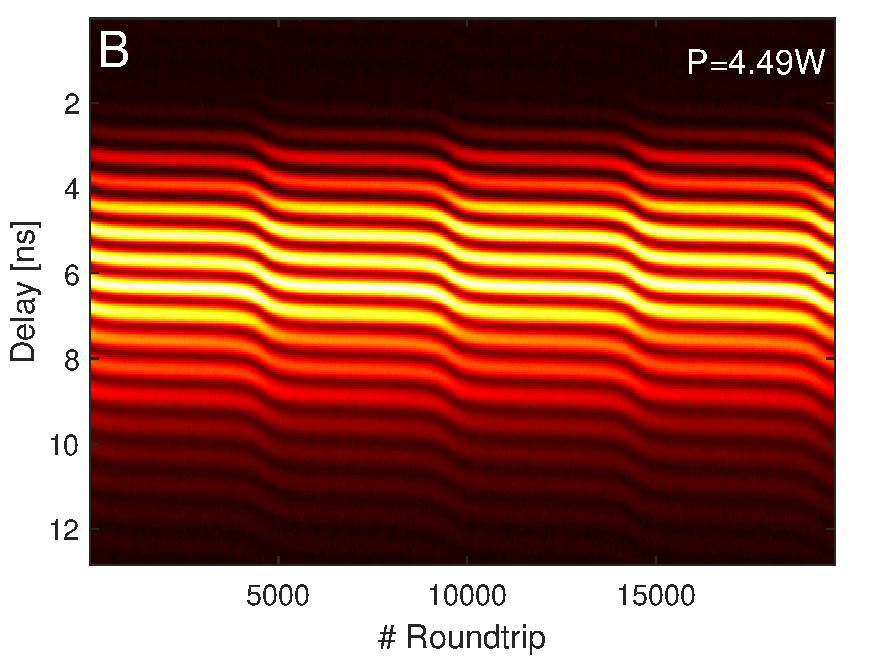
\includegraphics[width=0.49\textwidth]{figures/4ms_25GSA_400m_MLrun_Doppel4,49W_Ch_PWnoCB_scale}}
%   %\hfill
%   
%   \subfloat[]
%   {\includegraphics[width=0.49\textwidth]{figures/4ms_25GSA_400m_MLrun_Doppel4,45W_2_Ch_PWnoCB_scale}}
%   \hfill
%   \subfloat[]
%   {\includegraphics[width=0.49\textwidth]{figures/4ms_25GSA_400m_MLrun_Doppel4,34W_Ch_PWnoCB_scale}}
%   %\hfill
%   
%   \subfloat[]
%   {\includegraphics[width=0.49\textwidth]{figures/4ms_25GSA_400m_MLrun_Doppel4,3W_Ch_PWnoCB_scale}}
%   \hfill
%   \subfloat[]
%   {\includegraphics[width=0.49\textwidth]{figures/4ms_25GSA_400m_MLrun_Doppel4,2W_Ch_PWnoCB_scale}}
%   \caption{Verringerung der Pumpleistung: Von einer festen Phase über Stufen zu einer annähernd linear durchlaufenden Phase.}
%   \label{fig:165014steps_scale}
%\end{figure}

%\clearpage

\subsection{Dreifach-Pulse}
In Abbildung \ref{fig:Triplett} ist die spektrale Entwicklung sowie die Autokorrelation vier verschiedener Triplett-Zustände dargestellt, die sich nach mehrmaliger Störung aus dem cw-Betrieb einstellen.
In der Autokorrelation zeigen sich drei Abstände: der Abstand zwischen dem ersten und zweiten, zweiten und dritten sowie dem ersten und dritten Puls.
Auffällig ist, dass nur bestimmte Pulsabstände vorkommen: 110\,fs, 165\,fs, 265\,fs sowie 320\,fs.
Diese Abstände sind etwas größer als die in \cite{kitano_stable_1998} für zwei 15\,fs-Pulse gemessenen Abstände von 98\,fs, 164\,fs, 259\,fs sowie 312\,fs.
Die hier betrachteten Pulse sind daher wahrscheinlich ein wenig länger.
Im Spektrum lässt sich erkennen, dass die relativen Phasen oszillatorisches Verhalten sowie kontinuierliches Anwachsen aufweisen.
Wird die Pumpleistung verringert, stirbt einer der Pulse aus.
Die verbleibenden Beiden ändern ihren Abstand nicht grundlegend.
Dieser neue Zustand ist also auch stabil und verdeutlicht noch einmal die nur diskret vorkommenden Pulsabstände.
\begin{figure}[!htb]
   \centering
   \captionsetup[subfigure]{labelformat=empty}
   \captionsetup[subfloat]{farskip=-13pt,captionskip=0pt}
   \subfloat[]{\includegraphics[width=0.49\textwidth]{figures/4ms_25GSA_400m_MLrun_Triplett_Ch}}
   \hfill
   \subfloat[]
   {\includegraphics[width=0.49\textwidth]{figures/4ms_25GSA_400m_MLrun_Triplett_Ch_autocorr}}
   %\hfill
   
   \subfloat[]
   {\includegraphics[width=0.49\textwidth]{figures/4ms_25GSA_400m_MLrun_Triplett2_Ch}}
   \hfill
   \subfloat[]
   {\includegraphics[width=0.49\textwidth]{figures/4ms_25GSA_400m_MLrun_Triplett2_Ch_autocorr}}
   %\hfill
   
   \subfloat[]
   {\includegraphics[width=0.49\textwidth]{figures/4ms_25GSA_400m_MLrun_Triplett_3_Ch}}
   \hfill
   \subfloat[]
   {\includegraphics[width=0.49\textwidth]{figures/4ms_25GSA_400m_MLrun_Triplett_3_Ch_autocorr}}
   %\hfill
   
   \subfloat[]
   {\includegraphics[width=0.49\textwidth]{figures/4ms_25GSA_400m_MLrun_Triplett_4_Ch}}
   \hfill
   \subfloat[]
   {\includegraphics[width=0.49\textwidth]{figures/4ms_25GSA_400m_MLrun_Triplett_4_Ch_autocorr}}
   \caption{Verschiedene Triplett-Zustände: Spektrum und daraus berechntete Autokorrelation.
   Im Vergleich sind diskrete Pulsabstände zu erkennen.}
   \label{fig:Triplett}
\end{figure}

\clearpage

\section{Startdynamiken}
\label{sec:start}
In diesem Abschnitt werden die zwei beobachteten Prozesse vorgestellt, die zur Entstehung stabiler Doppelpulszustände führen:
Zwei Fluktuationen wachsen nahezu gleichzeitig zu Femtosekundenpulsen an, sind aber mehrere 100\,ps entfernt und nähern sich auf einer relativ langen Zeitskala an.
Bei dem anderen Voragang wächst ein Puls so schnell an, dass die Selbstphasenmodulation dazu führt, dass sich dieser aufspaltet.
Außerdem werden kurzlebige, sich so gebildete Doppelpulse beobachtet.

\subsection{Getrennte Starts}
In \cite{herink_resolving_2016} wird dargestellt, wie eine Pikosekunden-Fluktuation  spektral breiter, also kürzer wird und schließlich in einem Femtosekundenpuls endet.

In Abbildung \ref{fig:StartGetrennt} ist sowohl das undispergierte als auch das dispergierte Signal während der Entstehung zweier, weit entfernter Femtosekundenpulse zu sehen.
Das dispergierte Signal repräsentiert anfangs nicht das Spektrum, sondern stellt einen spektral-temporale Sicht dar.
So kann man anfangs die vielen Fluktuationen erkennen, die durch den Resonator propagieren.

Neu ist hier, dass einige Fluktuationen nach der Ausbildung des ersten Femtosekundenpulses nicht aussterben, sodass eine von diesen auch in die Modenkopplung übergehen kann.
Erst dann propagieren nur diese beiden Pulse durch den Resonator.

\begin{figure}[!htb]
   \centering
%   \captionsetup[subfigure]{labelformat=empty}
%   \captionsetup[subfloat]{farskip=-10pt,captionskip=0pt}   
   \subfloat[Undispergiertes Signal]
   {\includegraphics[width=0.49\textwidth]{figures/160518_205904_Doppelstart_undisp}}
   \hfill
   \subfloat[Dispergiertes Signal]
   {\includegraphics[width=0.49\textwidth]{figures/160518_205904_Doppelstart_spec}}
   \caption{Innerhalb von etwa $10^4$ Laserumläufen wachsen zwei Pikosekunden-Fluktuationen zu modengekoppelten Pulsen an.
   Der Pulsabstand beträgt anfangs ca. 430\,ps.}
   \label{fig:StartGetrennt}
\end{figure}
Das undispergierte Signal wird für die Ermittlung der wichtigsten Eigenschaften der beiden Pulse  verwendet: Die Entwicklung der Pulsenergien sowie des Pulsabstandes sind in Abbildung \ref{fig:StartGetrenntAusw} dargestellt.
Dabei wird über 50 Laserumläufe geglättet.
Zur Bestimmung der Pulsenergien wird für beide Puls die Höhe des Peaks im undispergierten Signal bestimmt.
Dabei sollte beachtet werden, dass die Photodiode nach einem Puls noch nachschwingt bzw. langsamer abfällt.
Dies bedeutet, dass die Energie des zweiten Pulses tendenziell überschätzt wird.
Der bestimmte Energieunterschied könnte also noch etwas größer sein.

Es kann beobachtet werden, dass die beiden Pulse sich näher kommen.
Dies kann man darauf zurückführen, dass der hintere und somit schwächere Puls aufgrund des Kerr-Effektes schneller durch den Laserkristall propagiert und sich daher der Pulsabstand verringert.

\begin{figure}[!htb]
   \centering
%   \captionsetup[subfigure]{labelformat=empty}
%   \captionsetup[subfloat]{farskip=-10pt,captionskip=0pt}   
   \subfloat[Startphase der beiden Pulse.]
   {\includegraphics[scale=0.29]{figures/2fachStartPeak}}
   \hfill
   \subfloat[Der zweite Puls ist etwas schwächer, sodass sich der Pulsabstand verringert.]
   {\includegraphics[scale=0.29]{figures/2fachStartPeakDist}}
   \caption{Auswertung der 2 getrennt startenden Femtosekundenpulse aus Abb. \ref{fig:StartGetrennt}: Entwicklung der beiden Pulsenenergien sowie des Pulsabstandes.}
   \label{fig:StartGetrenntAusw}
\end{figure}

\clearpage
\subsection{Annäherung}
Der Zeitpunkt, bei dem sich obige Pulse auf unter 1\,ps angenähert haben, kann leider nicht mehr aufgenommen werden, da dazu der Speicher des Oszilloskop nicht genügt.
Nimmt man obige Rate von ca. 20\,ps auf 3\,ms an, würde dies mehr als 60\,ms dauern.
Stattdessen kann aber auf eine solche Annäherung getriggert werden.
Dazu wird das dispergierte Signal verwendet, denn ein solcher Pulsabstand führt zu Modulationen im Spektrum, sodass die Peakspannung dieses Signals ansteigt und schließlich über dem eingestellten Grenzwert liegt.
In Abbildung \ref{fig:StartAnnaeherung} wird das Spektrum sowie die daraus berechnete Autokorrelation einer solchen Annäherung dargestellt.
Auffällig ist, dass der Pulsabstand nicht linear abnimmt, sondern leicht stufenförmig.
Die relative Phase nimmt beschleunigend zu, bis die nächste Stufe erreicht ist.
Die stabileren Abstände sind vergleichbar mit den diskreten Pulsabständen, die bei den Triplett-Zuständen auftreten.
Ein Endabstand von ca. 170\,fs sowie eine feste relative Phase stellen sich schließlich ein.
\begin{figure}[!htb]
	\centering
	\includegraphics[width=0.9\textwidth]{figures/4ms_25GSA_400m_MLstart_Doppelpulse2_Annaeherung_280500}
	\caption{Pulsannäherung bis ein stabiler Doppelpulszustand erreicht ist\\
	(\textit{oben:} Spektrale Entwicklung, \textit{unten:} Autokorrelation).}
	\label{fig:StartAnnaeherung}
\end{figure}

Der oben abgebildete Annäherunsprozess kann auch mit einer anderen Geschwindigkeit ablaufen:
Die Autokorrelation der zwei Extremfälle sind in Abbildung \ref{fig:StartAnnaehrung2} zu sehen.
Nähern sich die beiden Pulse sehr langsam an, können diskrete Pulsabstände beobachtet werden, die schon bei den Triplett-Zuständen beschrieben wurden.
So verharren die beiden Pulse längere Zeit bei diesen Abständen, bevor sie sich weiter annähern und schließlich der stabile Zustand gefunden wird.
Dies deutet darauf hin, dass die Pumpleistung für die größeren Pulsabstände zu niedrig ist.

Im anderen Fall nähern sich die beiden Pulse sehr schnell an, der Intensitätsunterschied ist also sehr groß.
Dabei kommt es zu einer Abstoßung, der Pulsabstand vergrößert sich also nochmal bevor er sich wieder verkleinert und ein stabiles Pulspaares gebildet wird.
Dieser Prozess ähnelt der Abstoßung aus Abbildung \ref{fig:rBF457_autocorr_zoom}.
Hier dient dies eventuell dem Energieaustausch, sodass die Bedingungen für einen stabilen Zustand hergestellt werden können.
\begin{figure}[!htb]
   \centering
%   \captionsetup[subfigure]{labelformat=empty}
%   \captionsetup[subfloat]{farskip=-10pt,captionskip=0pt}   
   \subfloat[Langsame Annäherung mit vielen semistabilen Pulsabständen.]
   {\includegraphics[width=0.49\textwidth]{figures/4ms_25GSA_400m_MLstart_Doppel6_autoCorr_stepWiseCloser_188300.pdf}}
   \hfill
   \subfloat[Schnelle Annäherung mit Abstoßung vor stabilem Doppelpulszustand.]
   {\includegraphics[width=0.49\textwidth]{figures/4ms_25GSA_400m_MLstart_Doppelpulse_Annaeherung_248000.pdf}}
   \caption{Autokorrelation zweier beispielhafter Annäherungen.}
   \label{fig:StartAnnaehrung2}
\end{figure}

\clearpage
\subsection{Aufspalten eines Pulses}
Nachdem in den vorigen Abschnitten gezeigt wurde, wie sich zwei, anfangs weit entfernte Pulse annähern und schließlich einen stabilen Doppelpulszustand formen, soll hier nun das Gegenteil illustriert werden: das Aufspalten eines Pulses wie es beispielhaft in Abbildung \ref{fig:Splitting} dargestellt ist.
Während das Spektrum breiter wird, sind gleichzeitig schon Modulationen auf diesem zu sehen.
Es handelt sich also um Doppelpulse, die sich voneinander entfernen.
Zu erkennen ist außerdem, dass die Änderungsrate der relativen Phase anfangs positiv ist. Wenn sich jedoch der stabile Pulsabstand einstellt, wird diese Rate leicht negativ.
Dies lässt darauf schließen, dass zuerst der spätere Puls der stärkere ist und sich der erste aufgrund des Kerr-Effektes entfernt.
Ist der Pulsabstand groß genug, findet ein Energieaustausch statt, der erste Puls erstarkt und ist schließlich stärker als der zweite Puls.
Der Abstand stabilisiert sich.
%Wenn eine Pikosekunden-Fluktuation 
\begin{figure}[!htb]
   \centering
   \includegraphics[width=\textwidth]{figures/4ms_25GSA_400m_Mlstart_Doppelpulse4_Splitting_93800}
   \caption{Anwachsen einer Pikosekunden-Fluktuation und gleichzeitiges Aufspalten des sich ausbildenden Femtoesekundenpulses (\textit{oben:} Spektrale Entwicklung, \textit{unten:} Autokorrelation).}
   \label{fig:Splitting}
\end{figure}

\clearpage
\subsection{Transiente Doppelpulse}
Der hier vorgestellte Fall kurzlebiger Doppelpulse ist sehr selten, so konnte er bisher nur zweimal beobachtet werden.
Der Resonator war dabei auf den Einzelpulsbetrieb justiert.
In Abbildung \ref{fig:TransientDoppel} ist zu erkennen, dass sich der entstehende Puls aufspaltet und die beiden resultierenden Pulse über die gesamte Lebensdauer des Doppelpulszustandes einen konstanten Abstand von etwa 265\,fs aufweisen.
Nach ca. 2000 Laserumläufen, also viel länger als die Lebensdauer des oberen Laserniveaus von $3.2\,\si{\micro\second}$, wird einer der beiden Pulse länger und stirbt aus.
Es wird vermutet, dass dies der spätere Puls ist, da dieser eine geringere Besetzungsinversion im Kristall vorfindet.
Da hier aber nur die Autokorrelation gemessen werden kann, kann dies nicht verifiziert werden.
\begin{figure}[!htb]
   \centering
   \captionsetup[subfigure]{labelformat=empty}
   \captionsetup[subfloat]{farskip=-10pt,captionskip=0pt}   
   \subfloat[]
   {\includegraphics[width=0.49\textwidth]{figures/4ms_25GSA_400m_MLstart_negDisp2e_Doppeltransient_spec}}
   \hfill
   \subfloat[]
   {\includegraphics[width=0.49\textwidth]{figures/4ms_25GSA_400m_MLstart_negDisp2e_Doppeltransient_autoCorr}}
   
   \subfloat[]
   {\includegraphics[width=0.49\textwidth]{figures/4ms_25GSA_400m_MLstart_negDisp2e_Doppeltransient_autoCorr_zoom1}}
   \hfill
   \subfloat[]
   {\includegraphics[width=0.49\textwidth]{figures/4ms_25GSA_400m_MLstart_negDisp2e_Doppeltransient_autoCorr_zoom2}}
   \caption{Transiente Doppelpulse: Nach Aufspalten in zwei Pulse und mehr als 2000 Laserumläufen in einem semistabilen Doppelpulszustand stirbt einer der beiden Pulse aus (\textit{oben links:} Spektrale Entwicklung, \textit{oben rechts:} Autokorrelation, \textit{unten:} Entstehen und Aussterben als Ausschnitt der Autokorrelation).}
   \label{fig:TransientDoppel}
\end{figure}

Die Abbildung \ref{fig:TransientSplittingAusw} zeigt die zeitliche Entwicklung der emittierten Energie pro Roundtrip.
Bei der Ausbildung der Femtosekundenpulse kommt es zu Relaxationsoszillationen.
Danach ist die Energie beider Pulse konstant und liegt etwa 18.5\% über der des Einzelpulses, der nach dem Aussterben des anderen alleine durch den Laser propagiert.
Die relative Phase wächst jedoch beschleunigt an.
Dies deutet darauf hin, dass das Ungleichgewicht der beiden Pulse zunimmt: Der erste Puls gewinnt kontinuierlich an Energie, während der zweite langsam schwächer wird.
Fällt die Pulsenergie unter einen bestimmten Wert, beschleunigt sich dieser Prozess dramatisch und der Puls stirbt aus.
Der überlebende Puls kann nun spektral breiter und energiereicher werden.
\begin{figure}[!htb]
	\centering
	\includegraphics[width=0.8\textwidth]{figures/TransientSplittingAusw}
	\caption{Transiente Doppelpulse: Während die Gesamtenergie beider Pulse lange konstant ist, lässt die Zunahme der Änderungsrate der relativen Phase auf ein Anstieg des Ungleichgewichts zwischen beiden Pulsen schließen.}
	\label{fig:TransientSplittingAusw}
\end{figure}

\clearpage
\section{Automodulationen}
In diesem Abschnitt wird ein weiterer interessanter Betriebsmodus präsentiert.
Dazu wird zuerst ein stabiler modengekoppelter Femtosekundenpuls erzeugt.
Danach wird der Abstand der beiden Fokussierspiegel (Stabilität) verringert, sodass die Verluste im Resonator größer werden.
Dies impliziert eine selbst erregte, starke Modulation der emittierten Leistung mit einer Modulationstiefe von mehr als 90\% (siehe Abb.\ref{fig:SelfQSwitch}).
Ein solcher Zyklus dauert etwa 172 Roundtrips, ca. $2.21\,\si{\micro\second}$, ist also etwas kürzer als die Lebensdauer des oberen Laserniveaus von $3.2\,\si{\micro\second}$.
Aufgrund des rapiden Leistungsanstiegs spaltet sich jedoch in vielen Fällen der gerade entstehende Puls auf, sodass für eine kurze Zeitspanne zwei Femtosekundenpulse im Laser propagieren.
Sogar drei Pulse entstehen manchmal.

\begin{figure}[!htb]
   \centering
   \includegraphics[width=0.85\textwidth]{figures/4ms_25GSA_400m_MLrun_ZitternHeftig_239100}
   \caption{Höhere Verluste im Resonator führen zu selbstverursachten Leistungsmodulationen auf einer Zeitskala der Lebensdauer des oberen Laserniveaus:
   Dabei können sich hier sogar bis zu drei Pulse ausbilden -- gefolgt von einer Phase nahezu keiner Laseremission. 
   (\textit{oben:} Spektrale Entwicklung, \textit{mitte:} Autokorrelation, \textit{unten:} Energie).}
   \label{fig:SelfQSwitch}
\end{figure}


\section{Simulation}
Einige der oben beschriebenen Vorgänge können auch simuliert werden.
Dazu wird das Modell aus Abschnitt \ref{sec:SimTheo} verwendet.
Im folgenden werden 3 verschiedene Dynamiken präsentiert, die sich nur durch kleine Änderungen der Simulationsparameter bzw. Anfangsbedingungen ergeben.
Die verwendeten Größen finden sich in Tabelle \ref{tab:SimParam} wieder.
Die so simulierten Doppelpulse weisen jeweils eine Pulslänge von etwa 28\,fs auf.
\begin{table}[!htb]
	\centering
	\begin{tabular}{|c|l|}
		\hline
		Größe & Wert\\
		\hline
		Zentralwellenlänge & $\lambda_0=800\,$nm\\	
		Brechungsindex @ $\lambda_0$ & $n=1.76$\\
		Kerr-Index & $n_2=3\cdot 10^{-20}\,\si{\meter^2\per\watt}$\\
		Kristalllänge & $x=2\,$mm\\
		Selbstphasenmodulation & $\beta=\frac{2\pi\cdot n_2\cdot 2x}{\lambda_0\cdot n}=5.36\cdot 10^{-16}\,\si{\meter^2\per\watt}$\\
		Selbstamplitudenmodulation & $\sigma=60$\\
		Modulationstiefe des sättigbaren Absorbers & $\gamma=0.24$\\
		Verluste & $\rho=3.3\%$\\
		Dispersion & $D_0=-50\,\si{\femto\second^2\per\meter}$\\
		Wirkungsquerschnitt Emission & $\sigma_g=41\,\si{\pico\meter^2}$\\
		Inverse spektrale Verstärkung & $t_f=2.5\,$fs\\	
		Sättigungsenergie & $E_s=\frac{h\,c}{\lambda_0\sigma_g}= 6.06\,\si{\kilo\joule\per\meter^2}$\\
		Resonatorperiode & $T_\text{cav}=12.8\,$ns\\
		Lebensdauer des oberen Niveaus & $T_r=3.2\,\si{\micro\second}$\\
		maximale Verstärkung & $\alpha_\text{max}=0.33$\\
		Pumpstrahlradius & $\omega_0=10\,\si{\micro\meter}$\\
		Pumpleistung & $P_\text{Pump}=4.6\,$W\\
		Absorptionswellenlänge & $\lambda_a=532\,$nm\\
		Absorptionsquerschnitt & $\sigma_a=20\,\si{\pico\meter^2}$\\
		& $P=\frac{P_\text{Pump}}{\pi\omega_0^2\cdot n}\cdot\frac{\sigma_a}{h\nu_a}\cdot T_\text{cav}=5.7\cdot 10^{-3}$\\
		\hline		
		Pulsform & 2 Gaußförmige Pulse\\
		Pulsamplitude & 1\\
		Pulslänge & 25\,fs\quad @ 1/e der Pulsamplitude\\
		Pulsabstand & $\tau_0=100,200\,$fs\\
		\hline
	\end{tabular}
	\caption{Simulationsparameter.}
	\label{tab:SimParam}
\end{table}

\clearpage
\subsection{Linear anwachsende Phase}
Der erste Fall behandelt den Fall einer linear anwachsenden relativen Phase aufgrund ungleicher Pulsamplituden, da hier die Verringerung der Besetzungsinversion durch den ersten Puls in Betracht gezogen wird.
In Abbildung \ref{fig:SimulationLinearPhase} ist die zeitliche sowie die spektrale Entwicklung dargestellt.
In Abb.\ref{fig:SimRBLinear} werden die Simulationsdaten ausgewertet, also die Pulsamplituden, der Pulsabstand und die relative Phase bestimmt.
So lässt sich die Simulation besser mit den Messdaten vergleichen.
Eine leichte Oszillation der Pulsamplituden und somit auch des Abstandes ist zu erkennen.
Das simulierte Verhalten hat starke Ähnlichkeiten zu Messungen wie in Abb.\ref{fig:165014steps} H, bei denen die Phase linear anwächst.
Der große Unterschied besteht jedoch in der Wahl des Pulsabstandes:
Während in den Messungen stets diskrete Abstände beobachtet wurden, wird in der Simulation der Anfangsabstand beibehalten.
Die beiden Pulse interagieren also nicht bzw. nur sehr schwach.
Die hier simulierte Zeitdauer beträgt aber auch nur 3000 Laserumläufe, während eine Messung etwa zwei Größenordnungen länger ist.
Eine längere Simulationsdauer ist also unter Umständen zur korrekten Beschreibung erforderlich, benötigt jedoch viel Speicherplatz.
Eine andere Erklärung ist die Änderung der Pulslänge während eines Laserumlaufes, welche stärker als angenommen sein könnte und somit im benutzen Modell keine Beachtung findet.
Dann wäre evtl. die Interaktion zwischen beiden Pulsen größer, sodass nur bestimmte Abstände stabil wären.
\begin{figure}[!htb]
   \centering
%   \captionsetup[subfigure]{labelformat=empty}
%   \captionsetup[subfloat]{farskip=-13pt,captionskip=0pt}   
   \subfloat[Entwicklung der zeitlichen Wellenform.]
   {\includegraphics[width=0.49\textwidth]{figures/SimulationRB_4,6W_200_time}}
   \hfill
   \subfloat[Spektrale Entwicklung.]
   {\includegraphics[width=0.49\textwidth]{figures/SimulationRB_4,6W_200_freq}}
   \caption{Simulation mit einem Anfangsabstand von $\tau_0=200\,$fs sowie einer Pumpleistung von $P_\text{Pump}=4.6\,$W. Die beiden Pulse  interagieren kaum, aufgrund leicht unterschiedlicher Pulsamplituden wächst die relative Phase zwischen beiden linear an.}
   \label{fig:SimulationLinearPhase}
\end{figure}

\begin{figure}[!htb]
	\centering
	\includegraphics[width=0.8\textwidth]{figures/SimRBLinear}
	\caption{Auswertung der Simulation aus Abb.\ref{fig:SimulationLinearPhase}: Energieverhältnis und Abstand der beiden Pulse ist nach einer kurzen Transiente nahezu konstant, sodass die relative Phase linear anwächst.}
	\label{fig:SimRBLinear}
\end{figure}

%\clearpage
\subsection{Oszillatorisches Verhalten}
Der zweite simulierte Fall unterscheidet sich von obigem nur durch einen kleineren Anfangsabstand $\tau_0=100\,$fs.
Nun können die beiden Pulse interagieren und es kommt zu Abstoßungs- und Anziehungseffekten, welche in einer oszillatorischen Bewegung mit einer Periodendauer von 330 Laserumläufen enden (vgl. Abb.\ref{fig:SimulationOscillation}).
Dieses Verhalten führt auch dazu, dass sich die beiden Pulse im Simulationsfenster immer weiter nach vorne bewegen, also schneller durch den Resonator propagieren als  ein einzelner Puls.
Absolut gesehen ist dieser Effekt jedoch gering: So sind die Pulse bei 3000 Laserumläufen, also ca. 40\,\si{\micro\second}, etwa 300\,fs schneller.

In Abbildung \ref{fig:SimRBOszi} sind die beiden Pulsamplituden, die relative Phase und der Pulsabstand während der Oszillationszyklen dargestellt.
Zu erkennen ist, dass der zweite Puls in einem Fünftel des Zykluses stärker als der erste ist.
Etwa zeitgleich vergrößert sich der Pulsabstand.
Pro Zyklus gibt es zwei Punkte, an denen beide Pulse gleich stark sind und die Phase ein lokales Extremum hat.
Außerdem ändert sich die Phase bei einem hohen Intensitätsunterschied zwischen beiden Pulsen sehr schnell.
Beides zeigt klar, dass die Änderung der relativen Phase stark mit den Pulsamplituden verknüpft ist.
Ähnlich verhält es sich mit dem Abstand.
Gleiche Pulsamplituden haben jedoch keinen festen Pulsabstand zu Folge, die Änderung des Abstandes lässt sich also nicht nur durch den Kerr-Effekt erklären.

\begin{figure}[!htb]
   \centering
   %\captionsetup[subfigure]{labelformat=empty}
   %\captionsetup[subfloat]{farskip=-13pt,captionskip=0pt}
   \subfloat[Entwicklung der zeitlichen Wellenform.]
   {\includegraphics[width=0.49\textwidth]{figures/SimulationRB_4,6W_100_time}}
   \hfill
   \subfloat[Spektrale Entwicklung.]
   {\includegraphics[width=0.49\textwidth]{figures/SimulationRB_4,6W_100_freq}}
   \caption{Simulation ($\tau_0=100\,$fs, $P_\text{Pump}=4.6\,$W), bei der Abstand und relative Phase oszillieren, da sich die beiden Pulse immer wieder leicht abstoßen.}
   \label{fig:SimulationOscillation}
\end{figure}

\begin{figure}[!htb]
	\centering
	\includegraphics[width=0.83\textwidth]{figures/SimRBOszi1}
	\caption{Auswertung der Simulation aus Abb.\ref{fig:SimulationOscillation}: Das Amplitudenverhältnis der Pulse ist stark mit dem Pulsabstand und der relativen Phase verknüpft.}
	\label{fig:SimRBOszi}
\end{figure}

In Abbildung \ref{fig:SimRBOszi_IP} ist diese Oszillationsdynamik in die \textit{Interaction Plane} eingezeichnet, es ergibt sich ein geschlossener Orbit.
Zu beachten ist, dass der innere Halbkreis und der Abschnitt, in dem sich die beiden Pulse voneinander entfernen, sehr schnell durchlaufen wird.
Nur in einem Viertel der Oszillationsperiode wächst der Abstand an.
Vergleicht man den Pulsabstand, welcher stets zwischen 60 und 80 Femtosekunden liegt, mit dem aus ähnlichen Messungen wie in Abb.\ref{fig:interactionPlane}, ist er  in der Simulation kleiner und ändert sich prozentual stärker. 

\begin{figure}[!htb]
	\centering
	\includegraphics[width=0.75\textwidth]{figures/SimRB_4,6W_InteractionPlane_matlab.pdf}
	\caption{Oszillatorisches Verhalten in der Interaction Plane.}
	\label{fig:SimRBOszi_IP}
\end{figure}

%\clearpage
\subsection{Fester Abstand und feste Phase}
Der dritte Fall unterscheidet sich von den bereits diskutierten durch eine höhere Pumpleistung.
Dies führt dazu, dass die beiden Pulse einen festen Abstand und eine feste Phase, also einen wirklichen Endzustand, annehmen.
In Abbildung \ref{fig:SimulationFixed} ist dies sowohl im Spektrum als auch im Zeitsignal zu erkennen.
Durch Auswerten der Simulation (Abb.\ref{fig:SimRBFix}) erkennt man, dass der erste Puls im Endzustand nur ca. $2.5\permil$ stärker als der andere ist.
Außerdem lässt sich ablesen, dass die relative Phase etwa bei $\pi$ gelockt ist. 
Die beiden Pulse sind also sehr ähnlich, aber gegenphasig.
Die Simulation beginnt mit einem Annäherungsprozess, bei dem 10\,fs\,-\,Stufen beobachtet werden können.
Diese sind also sehr viel kleiner als die gemessenen Abstandsdifferenzen von ungefähr $60-100\,$fs.
Der Endabstand beträgt ca. 64\,fs, ist also nur etwa doppelt so groß wie die Pulslänge von 28\,fs (FWHM).
In den Messungen aus den Abbildungen \ref{fig:165014steps} A+B beträgt der Pulsabstand jedoch ca. 170\,fs bei vergleichbarer Pulslänge.
\begin{figure}[!htb]
   \centering
   %\captionsetup[subfigure]{labelformat=empty}
   %\captionsetup[subfloat]{farskip=-13pt,captionskip=0pt}
   \subfloat[Entwicklung der zeitlichen Wellenform.]
   {\includegraphics[width=0.49\textwidth]{figures/SimulationRB_4,8W_100_time}}
   \hfill
   \subfloat[Spektrale Entwicklung.]
   {\includegraphics[width=0.49\textwidth]{figures/SimulationRB_4,8W_100_freq}}
   \caption{Simulation ($\tau_0=100\,$fs, $P_\text{Pump}=4.8\,$W), bei der die Pumpleistung höher ist, sodass die beiden Pulse ihren Abstand und ihre relative Phase locken können.}
   \label{fig:SimulationFixed}
\end{figure}

\begin{figure}[!htb]
	\centering
	\includegraphics[width=0.75\textwidth]{figures/SimRBFixed}
	\caption{Auswertung der Simulation aus Abb.\ref{fig:SimulationFixed}: Nach einer stufenförmigen Annäherung sind die Pulsamplituden, der Pulsabstand sowie die relative Phase schließlich konstant. Die Pulse sind dabei gegenphasig.}
	%Zeitliche Entwicklung der Pulsamplituden sowie des Pulsabstandes und der relativen Phase.}
	\label{fig:SimRBFix}
\end{figure}

\chapter{Diskussion und Ausblick}
Es ließen sich -- im Einklang mit der Literatur -- diskrete Pulsabstände  beobachten.
Durch Messen des Spektrums in Echtzeit konnten jedoch spannende Phasen-, aber auch Abstandsdynamiken für die beiden kleinsten Pulsabstände enthüllt werden.
Außerdem wurde mit den wiederkehrend kollidierenden Pulsen (vgl. Abschnitt \ref{sec:bounce}) ein neuer Zustand beobachtet, der sich überhaupt nur mit Echtzeit-Methoden messen lässt.
Der Zustand zweier Pulse, die nahezu unabhängig voneinander durch den Resonator laufen, lässt sich durch unterschiedliche Pulsamplituden erklären, wurde jedoch zuvor noch nie beschrieben.

Trotzdem sind noch viele Fragen offen.
Für ein besseres Verständnis der verschiedenen Regime muss die Simulation in Einklang mit den Messdaten gebracht werden.
Zudem sind weitere Dynamiken nicht undenkbar.

In den nächsten beiden Abschnitten werden zwei weitere wichtige Fragen diskutiert, die sich vor allem mit dieser Echtzeit-Methode beantworten lassen:
Woher stammen die beobachteten Multipulse? Und was passiert, wenn sich zwei Pulse im Kristall begegnen?

\section{Woher stammen die Doppelpulse?}
Splitting?
Modelockt eine andere Fluktuation?
Welche Parameter legen den vorherrschenden Prozess fest?

\section{Begegnung von Pulsen im Kristall}
\label{sec:cpml}
Während der Messungen konnte das sogennante \textit{Colliding Pulse Modelocking} beobachtet werden.
Dabei laufen zwei Pulse im Laser umher, die sich im Laserkristall treffen und so den Kerr-Effekt beider Pulse sehen, sodass beide eine höhere Verstärkung erfahren.
Dieser Zustand ist sehr stabil und wurde zuerst von \cite{lai_multiple_1997} in einem Ti:Sa-Laser beschrieben.
Interessant ist nun der Prozess bevor dieser stabile Zustand erreicht wird.
Typischerweise modelockt eine Fluktuation, während die anderen Fluktuationen aber nicht völlig aussterben.
Eine weitere Fluktuation wächst nun an, sodass auch diese modelockt.
Daraufhin bewegen sich die beiden Pulse relativ zueinander, da sie nicht gleich stark sind und aufgrund des Kerr-Effektes unterschiedliche optische Weglängen im Laser haben.
Dies geschieht auf einer relativ langen Zeitskala (Größenordnung $~100\,$ms), ist also mit einer normalen Messung (nur 4\,ms) nicht aufzunehmen.
Dazu müsste in den \textit{FastFrame}-Mode gewechselt werden, mit dem jedoch nicht jeder Puls aufgenommen werden kann.
Außerdem ist bei solch großen Pulsabständen das undispergierte Signal das aussagekräftigere.
Die Genauigkeit liegt dort aber nur bei ca. $10\,$ps.

Interessant zu beobachten wäre nun, wie der schwächere Puls die Relativbewegung beendet.
Gleichen sich beide Pulse nur in ihrer Intensität an, dass sie beide genau dann gleich stark sind, wenn sie den perfekten Abstand zueinander haben?
Oder ist eine abklingende Schwingung um diesen zu beobachten?
Ist dieser Abstand stabil oder gibt es auch später noch Oszillationen?

Um all diese Fragen zu beantworten, könnte man den Strahl aufspalten und den einen Teil so verzögern, dass der erste Puls in diesem Arm zeitgleich mit dem zweiten Puls im kürzeren Abschnitt überlappt.
Nun ist die Abstandsinformation auch wieder im Spektrum kodiert und der Abstand zwischen beiden Pulsen kann genau gemessen werden.


\appendix
\chapter{Femtolasers Rainbow CEP HP}
\begin{figure}[!htb]
	\centering
	\includegraphics[width=0.55\textwidth]{figures/RainbowSetupManual.png}
	\caption{CAD-Zeichnung des Oszillators aus Femtolasers, \textit{Femtosource Rainbow HP CEP - Users Manual v1.1}.}
\end{figure}
%\chapter{Matlab-Code}
%\section{Darstellung der Messdaten}
%
%\section{Simulation}
%\lstinputlisting[style=Matlab-editor]{SimulationRBcomment.m}

\cleardoublepage
%% Bibliographie. Das Argument muss der Name der BIBTeX-Datenbank stehen.
%% Ein Beispiel fuer eine solche Datenbank finden Sie in bthesis_datenbank.bib
\bibliography{test}

\chapter*{Danksagung}
Ganz besonders bedanke ich mich bei Prof. Dr. Claus Ropers, der diese Arbeit möglich gemacht hat.

Ein besonderes Dankeschön geht an Herrn Dr. Christoph Bollig von \textit{Abacus Laser} für seine schnelle, technische Unterstützung.

Außerdem bedanke ich mich bei den Mitarbeitern der Elekronik-Werkstatt sowie Andreas Juretzko von der feinmechanischen Werkstatt des 4.Physikalischen Instituts für ihre kompetente und schnelle Unterstützung.

%% Dieser Befehl MUSS am Ende stehen und erzeugt die Erklaerung ueber die
%% benutzten Mittel
\cleardoublepage
\Declaration
\end{document}
